% **************************************************************************************************************
% A Classic Thesis Style
% An Homage to The Elements of Typographic Style
%
% Copyright (C) 2015 André Miede http://www.miede.de
%
% If you like the style then I would appreciate a postcard. My address 
% can be found in the file ClassicThesis.pdf. A collection of the 
% postcards I received so far is available online at 
% http://postcards.miede.de
%
% License:
% This program is free software; you can redistribute it and/or modify
% it under the terms of the GNU General Public License as published by
% the Free Software Foundation; either version 2 of the License, or
% (at your option) any later version.
%
% This program is distributed in the hope that it will be useful,
% but WITHOUT ANY WARRANTY; without even the implied warranty of
% MERCHANTABILITY or FITNESS FOR A PARTICULAR PURPOSE.  See the
% GNU General Public License for more details.
%
% You should have received a copy of the GNU General Public License
% along with this program; see the file COPYING.  If not, write to
% the Free Software Foundation, Inc., 59 Temple Place - Suite 330,
% Boston, MA 02111-1307, USA.
%
% **************************************************************************************************************
\RequirePackage{fix-cm} % fix some latex issues see: http://texdoc.net/texmf-dist/doc/latex/base/fixltx2e.pdf
\documentclass[ twoside,openright,titlepage,numbers=noenddot,headinclude,%1headlines,% letterpaper a4paper
                footinclude=true,cleardoublepage=empty,abstractoff, % <--- obsolete, remove (todo)
                BCOR=5mm,fontsize=11pt,%11pt,a4paper,%
                ngerman,american,%
                ]{scrreprt}

%********************************************************************
% Note: Make all your adjustments in here
%*******************************************************
% ****************************************************************************************************
% classicthesis-config.tex 
% formerly known as loadpackages.sty, classicthesis-ldpkg.sty, and classicthesis-preamble.sty 
% Use it at the beginning of your ClassicThesis.tex, or as a LaTeX Preamble 
% in your ClassicThesis.{tex,lyx} with % ****************************************************************************************************
% classicthesis-config.tex 
% formerly known as loadpackages.sty, classicthesis-ldpkg.sty, and classicthesis-preamble.sty 
% Use it at the beginning of your ClassicThesis.tex, or as a LaTeX Preamble 
% in your ClassicThesis.{tex,lyx} with % ****************************************************************************************************
% classicthesis-config.tex 
% formerly known as loadpackages.sty, classicthesis-ldpkg.sty, and classicthesis-preamble.sty 
% Use it at the beginning of your ClassicThesis.tex, or as a LaTeX Preamble 
% in your ClassicThesis.{tex,lyx} with \input{classicthesis-config}
% ****************************************************************************************************  
% If you like the classicthesis, then I would appreciate a postcard. 
% My address can be found in the file ClassicThesis.pdf. A collection 
% of the postcards I received so far is available online at 
% http://postcards.miede.de
% ****************************************************************************************************


% ****************************************************************************************************
% 0. Set the encoding of your files. UTF-8 is the only sensible encoding nowadays. If you can't read
% äöüßáéçèê∂åëæƒÏ€ then change the encoding setting in your editor, not the line below. If your editor
% does not support utf8 use another editor!
% ****************************************************************************************************
\PassOptionsToPackage{utf8}{inputenc}
	\usepackage{inputenc}

% ****************************************************************************************************
% 1. Configure classicthesis for your needs here, e.g., remove "drafting" below 
% in order to deactivate the time-stamp on the pages
% ****************************************************************************************************
\PassOptionsToPackage{eulerchapternumbers,listings,drafting,%
					 pdfspacing,floatperchapter,%linedheaders,%
					 subfig,beramono,eulermath,parts}{classicthesis}                                        
% ********************************************************************
% Available options for classicthesis.sty 
% (see ClassicThesis.pdf for more information):
% drafting
% parts nochapters linedheaders
% eulerchapternumbers beramono eulermath pdfspacing minionprospacing
% tocaligned dottedtoc manychapters
% listings floatperchapter subfig
% ********************************************************************


% ****************************************************************************************************
% 2. Personal data and user ad-hoc commands
% ****************************************************************************************************
\newcommand{\myTitle}{New Advances in Statistical Neuroimage Processing\xspace}
\newcommand{\mySubtitle}{TESIS DOCTORAL\xspace}
\newcommand{\myDegree}{Doctor en Ingeniería (Dr.-Ing.)\xspace}
\newcommand{\myName}{Francisco Jes\'us Mart\'inez Murcia\xspace}
\newcommand{\myProf}{Juan Manuel G\'orriz S\'aez\xspace}
\newcommand{\myOtherProf}{Javier Ram\'irez P\'erez de Inestrosa\xspace}
\newcommand{\mySupervisor}{Put name here\xspace}
\newcommand{\myFaculty}{Escuela Técnica Superior de Ingenierías Informática y de Telecomunicación\xspace}
\newcommand{\myDepartment}{Departamento de Teoría de la Señal, Telemática y Comunicaciones\xspace}
\newcommand{\myUni}{Universidad de Granada\xspace}
\newcommand{\myLocation}{Granada\xspace}
\newcommand{\myTime}{Junio 2017\xspace}
\newcommand{\myVersion}{version 4.2\xspace}

% ********************************************************************
% Setup, finetuning, and useful commands
% ********************************************************************
\newcounter{dummy} % necessary for correct hyperlinks (to index, bib, etc.)
\newlength{\abcd} % for ab..z string length calculation
\providecommand{\mLyX}{L\kern-.1667em\lower.25em\hbox{Y}\kern-.125emX\@}
\newcommand{\ie}{i.\,e.}
\newcommand{\Ie}{I.\,e.}
\newcommand{\eg}{e.\,g.}
\newcommand{\Eg}{E.\,g.} 
% ****************************************************************************************************


% ****************************************************************************************************
% 3. Loading some handy packages
% ****************************************************************************************************
% ******************************************************************** 
% Packages with options that might require adjustments
% ******************************************************************** 
%\PassOptionsToPackage{ngerman,american}{babel}   % change this to your language(s)
% Spanish languages need extra options in order to work with this template
\PassOptionsToPackage{spanish,es-lcroman}{babel}
	\usepackage{babel}                  

\usepackage{csquotes}
\PassOptionsToPackage{%
    backend=biber,  %instead of bibtex
	%backend=bibtex8, bibencoding=ascii,%
	language=auto,%
	style=numeric-comp,%
    %style=authoryear-comp, % Author 1999, 2010
    %bibstyle=authoryear,dashed=false, % dashed: substitute rep. author with ---
    sorting=nyt, % name, year, title
    maxbibnames=10, % default: 3, et al.
    %backref=true,%
    natbib=true % natbib compatibility mode (\citep and \citet still work)
}{biblatex}
    \usepackage{biblatex}

\PassOptionsToPackage{fleqn}{amsmath}       % math environments and more by the AMS 
    \usepackage{amsmath}

% ******************************************************************** 
% General useful packages
% ******************************************************************** 
\PassOptionsToPackage{T1}{fontenc} % T2A for cyrillics
    \usepackage{fontenc}     
\usepackage{textcomp} % fix warning with missing font shapes
\usepackage{scrhack} % fix warnings when using KOMA with listings package          
\usepackage{xspace} % to get the spacing after macros right  
\usepackage{mparhack} % get marginpar right
\usepackage{fixltx2e} % fixes some LaTeX stuff --> since 2015 in the LaTeX kernel (see below)
%\usepackage[latest]{latexrelease} % will be used once available in more distributions (ISSUE #107)
\PassOptionsToPackage{printonlyused,smaller}{acronym} 
    \usepackage{acronym} % nice macros for handling all acronyms in the thesis
    %\renewcommand{\bflabel}[1]{{#1}\hfill} % fix the list of acronyms --> no longer working
    %\renewcommand*{\acsfont}[1]{\textsc{#1}} 
    \renewcommand*{\aclabelfont}[1]{\acsfont{#1}}
% ****************************************************************************************************
\usepackage{listings}
\usepackage{multirow}
\usepackage{rotating}

% ****************************************************************************************************
% 4. Setup floats: tables, (sub)figures, and captions
% ****************************************************************************************************
\usepackage{tabularx} % better tables
    \setlength{\extrarowheight}{3pt} % increase table row height
\newcommand{\tableheadline}[1]{\multicolumn{1}{c}{\spacedlowsmallcaps{#1}}}
\newcommand{\myfloatalign}{\centering} % to be used with each float for alignment
\usepackage{caption}
% Thanks to cgnieder and Claus Lahiri
% http://tex.stackexchange.com/questions/69349/spacedlowsmallcaps-in-caption-label
% [REMOVED DUE TO OTHER PROBLEMS, SEE ISSUE #82]    
%\DeclareCaptionLabelFormat{smallcaps}{\bothIfFirst{#1}{~}\MakeTextLowercase{\textsc{#2}}}
%\captionsetup{font=small,labelformat=smallcaps} % format=hang,
\captionsetup{font=small} % format=hang,
\usepackage{subfig}  
% ****************************************************************************************************


% ****************************************************************************************************
% 5. Setup code listings
% ****************************************************************************************************
\usepackage{listings} 
%\lstset{emph={trueIndex,root},emphstyle=\color{BlueViolet}}%\underbar} % for special keywords
\lstset{language=[LaTeX]Tex,%C++,
    morekeywords={PassOptionsToPackage,selectlanguage},
    keywordstyle=\color{RoyalBlue},%\bfseries,
    basicstyle=\small\ttfamily,
    %identifierstyle=\color{NavyBlue},
    commentstyle=\color{Green}\ttfamily,
    stringstyle=\rmfamily,
    numbers=none,%left,%
    numberstyle=\scriptsize,%\tiny
    stepnumber=5,
    numbersep=8pt,
    showstringspaces=false,
    breaklines=true,
    %frameround=ftff,
    %frame=single,
    belowcaptionskip=.75\baselineskip
    %frame=L
} 
% ****************************************************************************************************             


% ****************************************************************************************************
% 6. PDFLaTeX, hyperreferences and citation backreferences
% ****************************************************************************************************
% ********************************************************************
% Using PDFLaTeX
% ********************************************************************
\PassOptionsToPackage{pdftex,hyperfootnotes=false,pdfpagelabels}{hyperref}
    \usepackage{hyperref}  % backref linktocpage pagebackref
\pdfcompresslevel=9
\pdfadjustspacing=1 
\PassOptionsToPackage{pdftex}{graphicx}
    \usepackage{graphicx} 
 

% ********************************************************************
% Hyperreferences
% ********************************************************************
\hypersetup{%
    %draft, % = no hyperlinking at all (useful in b/w printouts)
    colorlinks=true, linktocpage=true, pdfstartpage=3, pdfstartview=FitV,%
    % uncomment the following line if you want to have black links (e.g., for printing)
    %colorlinks=false, linktocpage=false, pdfstartpage=3, pdfstartview=FitV, pdfborder={0 0 0},%
    breaklinks=true, pdfpagemode=UseNone, pageanchor=true, pdfpagemode=UseOutlines,%
    plainpages=false, bookmarksnumbered, bookmarksopen=true, bookmarksopenlevel=1,%
    hypertexnames=true, pdfhighlight=/O,%nesting=true,%frenchlinks,%
    urlcolor=webbrown, linkcolor=RoyalBlue, citecolor=webgreen, %pagecolor=RoyalBlue,%
    %urlcolor=Black, linkcolor=Black, citecolor=Black, %pagecolor=Black,%
    pdftitle={\myTitle},%
    pdfauthor={\textcopyright\ \myName, \myUni, \myFaculty},%
    pdfsubject={},%
    pdfkeywords={},%
    pdfcreator={pdfLaTeX},%
    pdfproducer={LaTeX with hyperref and classicthesis}%
}   

% ********************************************************************
% Setup autoreferences
% ********************************************************************
% There are some issues regarding autorefnames
% http://www.ureader.de/msg/136221647.aspx
% http://www.tex.ac.uk/cgi-bin/texfaq2html?label=latexwords
% you have to redefine the makros for the 
% language you use, e.g., american, ngerman
% (as chosen when loading babel/AtBeginDocument)
% ********************************************************************
\makeatletter
\@ifpackageloaded{babel}%
    {%
       \addto\extrasamerican{%
			\renewcommand*{\figureautorefname}{Figure}%
			\renewcommand*{\tableautorefname}{Table}%
			\renewcommand*{\partautorefname}{Part}%
			\renewcommand*{\chapterautorefname}{Chapter}%
			\renewcommand*{\sectionautorefname}{Section}%
			\renewcommand*{\subsectionautorefname}{Section}%
			\renewcommand*{\subsubsectionautorefname}{Section}%     
                }%
       \addto\extrasngerman{% 
			\renewcommand*{\paragraphautorefname}{Absatz}%
			\renewcommand*{\subparagraphautorefname}{Unterabsatz}%
			\renewcommand*{\footnoteautorefname}{Fu\"snote}%
			\renewcommand*{\FancyVerbLineautorefname}{Zeile}%
			\renewcommand*{\theoremautorefname}{Theorem}%
			\renewcommand*{\appendixautorefname}{Anhang}%
			\renewcommand*{\equationautorefname}{Gleichung}%        
			\renewcommand*{\itemautorefname}{Punkt}%
                }%  
            % Fix to getting autorefs for subfigures right (thanks to Belinda Vogt for changing the definition)
            \providecommand{\subfigureautorefname}{\figureautorefname}%             
    }{\relax}
\makeatother


% ****************************************************************************************************
% 7. Last calls before the bar closes
% ****************************************************************************************************
% ********************************************************************
% Development Stuff
% ********************************************************************
\listfiles
%\PassOptionsToPackage{l2tabu,orthodox,abort}{nag}
%   \usepackage{nag}
%\PassOptionsToPackage{warning, all}{onlyamsmath}
%   \usepackage{onlyamsmath}

% ********************************************************************
% Last, but not least...
% ********************************************************************
\usepackage{classicthesis} 
% ****************************************************************************************************


% ****************************************************************************************************
% 8. Further adjustments (experimental)
% ****************************************************************************************************
% ********************************************************************
% Changing the text area
% ********************************************************************
%\linespread{1.05} % a bit more for Palatino
%\areaset[current]{312pt}{761pt} % 686 (factor 2.2) + 33 head + 42 head \the\footskip
%\setlength{\marginparwidth}{7em}%
%\setlength{\marginparsep}{2em}%

% ********************************************************************
% Using different fonts
% ********************************************************************
%\usepackage[oldstylenums]{kpfonts} % oldstyle notextcomp
%\usepackage[osf]{libertine}
%\usepackage[light,condensed,math]{iwona}
%\renewcommand{\sfdefault}{iwona}
%\usepackage{lmodern} % <-- no osf support :-(
%\usepackage{cfr-lm} % 
%\usepackage[urw-garamond]{mathdesign} <-- no osf support :-(
%\usepackage[default,osfigures]{opensans} % scale=0.95 
%\usepackage[sfdefault]{FiraSans}
% ****************************************************************************************************

% ****************************************************************************************************  
% If you like the classicthesis, then I would appreciate a postcard. 
% My address can be found in the file ClassicThesis.pdf. A collection 
% of the postcards I received so far is available online at 
% http://postcards.miede.de
% ****************************************************************************************************


% ****************************************************************************************************
% 0. Set the encoding of your files. UTF-8 is the only sensible encoding nowadays. If you can't read
% äöüßáéçèê∂åëæƒÏ€ then change the encoding setting in your editor, not the line below. If your editor
% does not support utf8 use another editor!
% ****************************************************************************************************
\PassOptionsToPackage{utf8}{inputenc}
	\usepackage{inputenc}

% ****************************************************************************************************
% 1. Configure classicthesis for your needs here, e.g., remove "drafting" below 
% in order to deactivate the time-stamp on the pages
% ****************************************************************************************************
\PassOptionsToPackage{eulerchapternumbers,listings,drafting,%
					 pdfspacing,floatperchapter,%linedheaders,%
					 subfig,beramono,eulermath,parts}{classicthesis}                                        
% ********************************************************************
% Available options for classicthesis.sty 
% (see ClassicThesis.pdf for more information):
% drafting
% parts nochapters linedheaders
% eulerchapternumbers beramono eulermath pdfspacing minionprospacing
% tocaligned dottedtoc manychapters
% listings floatperchapter subfig
% ********************************************************************


% ****************************************************************************************************
% 2. Personal data and user ad-hoc commands
% ****************************************************************************************************
\newcommand{\myTitle}{New Advances in Statistical Neuroimage Processing\xspace}
\newcommand{\mySubtitle}{TESIS DOCTORAL\xspace}
\newcommand{\myDegree}{Doctor en Ingeniería (Dr.-Ing.)\xspace}
\newcommand{\myName}{Francisco Jes\'us Mart\'inez Murcia\xspace}
\newcommand{\myProf}{Juan Manuel G\'orriz S\'aez\xspace}
\newcommand{\myOtherProf}{Javier Ram\'irez P\'erez de Inestrosa\xspace}
\newcommand{\mySupervisor}{Put name here\xspace}
\newcommand{\myFaculty}{Escuela Técnica Superior de Ingenierías Informática y de Telecomunicación\xspace}
\newcommand{\myDepartment}{Departamento de Teoría de la Señal, Telemática y Comunicaciones\xspace}
\newcommand{\myUni}{Universidad de Granada\xspace}
\newcommand{\myLocation}{Granada\xspace}
\newcommand{\myTime}{Junio 2017\xspace}
\newcommand{\myVersion}{version 4.2\xspace}

% ********************************************************************
% Setup, finetuning, and useful commands
% ********************************************************************
\newcounter{dummy} % necessary for correct hyperlinks (to index, bib, etc.)
\newlength{\abcd} % for ab..z string length calculation
\providecommand{\mLyX}{L\kern-.1667em\lower.25em\hbox{Y}\kern-.125emX\@}
\newcommand{\ie}{i.\,e.}
\newcommand{\Ie}{I.\,e.}
\newcommand{\eg}{e.\,g.}
\newcommand{\Eg}{E.\,g.} 
% ****************************************************************************************************


% ****************************************************************************************************
% 3. Loading some handy packages
% ****************************************************************************************************
% ******************************************************************** 
% Packages with options that might require adjustments
% ******************************************************************** 
%\PassOptionsToPackage{ngerman,american}{babel}   % change this to your language(s)
% Spanish languages need extra options in order to work with this template
\PassOptionsToPackage{spanish,es-lcroman}{babel}
	\usepackage{babel}                  

\usepackage{csquotes}
\PassOptionsToPackage{%
    backend=biber,  %instead of bibtex
	%backend=bibtex8, bibencoding=ascii,%
	language=auto,%
	style=numeric-comp,%
    %style=authoryear-comp, % Author 1999, 2010
    %bibstyle=authoryear,dashed=false, % dashed: substitute rep. author with ---
    sorting=nyt, % name, year, title
    maxbibnames=10, % default: 3, et al.
    %backref=true,%
    natbib=true % natbib compatibility mode (\citep and \citet still work)
}{biblatex}
    \usepackage{biblatex}

\PassOptionsToPackage{fleqn}{amsmath}       % math environments and more by the AMS 
    \usepackage{amsmath}

% ******************************************************************** 
% General useful packages
% ******************************************************************** 
\PassOptionsToPackage{T1}{fontenc} % T2A for cyrillics
    \usepackage{fontenc}     
\usepackage{textcomp} % fix warning with missing font shapes
\usepackage{scrhack} % fix warnings when using KOMA with listings package          
\usepackage{xspace} % to get the spacing after macros right  
\usepackage{mparhack} % get marginpar right
\usepackage{fixltx2e} % fixes some LaTeX stuff --> since 2015 in the LaTeX kernel (see below)
%\usepackage[latest]{latexrelease} % will be used once available in more distributions (ISSUE #107)
\PassOptionsToPackage{printonlyused,smaller}{acronym} 
    \usepackage{acronym} % nice macros for handling all acronyms in the thesis
    %\renewcommand{\bflabel}[1]{{#1}\hfill} % fix the list of acronyms --> no longer working
    %\renewcommand*{\acsfont}[1]{\textsc{#1}} 
    \renewcommand*{\aclabelfont}[1]{\acsfont{#1}}
% ****************************************************************************************************
\usepackage{listings}
\usepackage{multirow}
\usepackage{rotating}

% ****************************************************************************************************
% 4. Setup floats: tables, (sub)figures, and captions
% ****************************************************************************************************
\usepackage{tabularx} % better tables
    \setlength{\extrarowheight}{3pt} % increase table row height
\newcommand{\tableheadline}[1]{\multicolumn{1}{c}{\spacedlowsmallcaps{#1}}}
\newcommand{\myfloatalign}{\centering} % to be used with each float for alignment
\usepackage{caption}
% Thanks to cgnieder and Claus Lahiri
% http://tex.stackexchange.com/questions/69349/spacedlowsmallcaps-in-caption-label
% [REMOVED DUE TO OTHER PROBLEMS, SEE ISSUE #82]    
%\DeclareCaptionLabelFormat{smallcaps}{\bothIfFirst{#1}{~}\MakeTextLowercase{\textsc{#2}}}
%\captionsetup{font=small,labelformat=smallcaps} % format=hang,
\captionsetup{font=small} % format=hang,
\usepackage{subfig}  
% ****************************************************************************************************


% ****************************************************************************************************
% 5. Setup code listings
% ****************************************************************************************************
\usepackage{listings} 
%\lstset{emph={trueIndex,root},emphstyle=\color{BlueViolet}}%\underbar} % for special keywords
\lstset{language=[LaTeX]Tex,%C++,
    morekeywords={PassOptionsToPackage,selectlanguage},
    keywordstyle=\color{RoyalBlue},%\bfseries,
    basicstyle=\small\ttfamily,
    %identifierstyle=\color{NavyBlue},
    commentstyle=\color{Green}\ttfamily,
    stringstyle=\rmfamily,
    numbers=none,%left,%
    numberstyle=\scriptsize,%\tiny
    stepnumber=5,
    numbersep=8pt,
    showstringspaces=false,
    breaklines=true,
    %frameround=ftff,
    %frame=single,
    belowcaptionskip=.75\baselineskip
    %frame=L
} 
% ****************************************************************************************************             


% ****************************************************************************************************
% 6. PDFLaTeX, hyperreferences and citation backreferences
% ****************************************************************************************************
% ********************************************************************
% Using PDFLaTeX
% ********************************************************************
\PassOptionsToPackage{pdftex,hyperfootnotes=false,pdfpagelabels}{hyperref}
    \usepackage{hyperref}  % backref linktocpage pagebackref
\pdfcompresslevel=9
\pdfadjustspacing=1 
\PassOptionsToPackage{pdftex}{graphicx}
    \usepackage{graphicx} 
 

% ********************************************************************
% Hyperreferences
% ********************************************************************
\hypersetup{%
    %draft, % = no hyperlinking at all (useful in b/w printouts)
    colorlinks=true, linktocpage=true, pdfstartpage=3, pdfstartview=FitV,%
    % uncomment the following line if you want to have black links (e.g., for printing)
    %colorlinks=false, linktocpage=false, pdfstartpage=3, pdfstartview=FitV, pdfborder={0 0 0},%
    breaklinks=true, pdfpagemode=UseNone, pageanchor=true, pdfpagemode=UseOutlines,%
    plainpages=false, bookmarksnumbered, bookmarksopen=true, bookmarksopenlevel=1,%
    hypertexnames=true, pdfhighlight=/O,%nesting=true,%frenchlinks,%
    urlcolor=webbrown, linkcolor=RoyalBlue, citecolor=webgreen, %pagecolor=RoyalBlue,%
    %urlcolor=Black, linkcolor=Black, citecolor=Black, %pagecolor=Black,%
    pdftitle={\myTitle},%
    pdfauthor={\textcopyright\ \myName, \myUni, \myFaculty},%
    pdfsubject={},%
    pdfkeywords={},%
    pdfcreator={pdfLaTeX},%
    pdfproducer={LaTeX with hyperref and classicthesis}%
}   

% ********************************************************************
% Setup autoreferences
% ********************************************************************
% There are some issues regarding autorefnames
% http://www.ureader.de/msg/136221647.aspx
% http://www.tex.ac.uk/cgi-bin/texfaq2html?label=latexwords
% you have to redefine the makros for the 
% language you use, e.g., american, ngerman
% (as chosen when loading babel/AtBeginDocument)
% ********************************************************************
\makeatletter
\@ifpackageloaded{babel}%
    {%
       \addto\extrasamerican{%
			\renewcommand*{\figureautorefname}{Figure}%
			\renewcommand*{\tableautorefname}{Table}%
			\renewcommand*{\partautorefname}{Part}%
			\renewcommand*{\chapterautorefname}{Chapter}%
			\renewcommand*{\sectionautorefname}{Section}%
			\renewcommand*{\subsectionautorefname}{Section}%
			\renewcommand*{\subsubsectionautorefname}{Section}%     
                }%
       \addto\extrasngerman{% 
			\renewcommand*{\paragraphautorefname}{Absatz}%
			\renewcommand*{\subparagraphautorefname}{Unterabsatz}%
			\renewcommand*{\footnoteautorefname}{Fu\"snote}%
			\renewcommand*{\FancyVerbLineautorefname}{Zeile}%
			\renewcommand*{\theoremautorefname}{Theorem}%
			\renewcommand*{\appendixautorefname}{Anhang}%
			\renewcommand*{\equationautorefname}{Gleichung}%        
			\renewcommand*{\itemautorefname}{Punkt}%
                }%  
            % Fix to getting autorefs for subfigures right (thanks to Belinda Vogt for changing the definition)
            \providecommand{\subfigureautorefname}{\figureautorefname}%             
    }{\relax}
\makeatother


% ****************************************************************************************************
% 7. Last calls before the bar closes
% ****************************************************************************************************
% ********************************************************************
% Development Stuff
% ********************************************************************
\listfiles
%\PassOptionsToPackage{l2tabu,orthodox,abort}{nag}
%   \usepackage{nag}
%\PassOptionsToPackage{warning, all}{onlyamsmath}
%   \usepackage{onlyamsmath}

% ********************************************************************
% Last, but not least...
% ********************************************************************
\usepackage{classicthesis} 
% ****************************************************************************************************


% ****************************************************************************************************
% 8. Further adjustments (experimental)
% ****************************************************************************************************
% ********************************************************************
% Changing the text area
% ********************************************************************
%\linespread{1.05} % a bit more for Palatino
%\areaset[current]{312pt}{761pt} % 686 (factor 2.2) + 33 head + 42 head \the\footskip
%\setlength{\marginparwidth}{7em}%
%\setlength{\marginparsep}{2em}%

% ********************************************************************
% Using different fonts
% ********************************************************************
%\usepackage[oldstylenums]{kpfonts} % oldstyle notextcomp
%\usepackage[osf]{libertine}
%\usepackage[light,condensed,math]{iwona}
%\renewcommand{\sfdefault}{iwona}
%\usepackage{lmodern} % <-- no osf support :-(
%\usepackage{cfr-lm} % 
%\usepackage[urw-garamond]{mathdesign} <-- no osf support :-(
%\usepackage[default,osfigures]{opensans} % scale=0.95 
%\usepackage[sfdefault]{FiraSans}
% ****************************************************************************************************

% ****************************************************************************************************  
% If you like the classicthesis, then I would appreciate a postcard. 
% My address can be found in the file ClassicThesis.pdf. A collection 
% of the postcards I received so far is available online at 
% http://postcards.miede.de
% ****************************************************************************************************


% ****************************************************************************************************
% 0. Set the encoding of your files. UTF-8 is the only sensible encoding nowadays. If you can't read
% äöüßáéçèê∂åëæƒÏ€ then change the encoding setting in your editor, not the line below. If your editor
% does not support utf8 use another editor!
% ****************************************************************************************************
\PassOptionsToPackage{utf8}{inputenc}
	\usepackage{inputenc}

% ****************************************************************************************************
% 1. Configure classicthesis for your needs here, e.g., remove "drafting" below 
% in order to deactivate the time-stamp on the pages
% ****************************************************************************************************
\PassOptionsToPackage{eulerchapternumbers,listings,drafting,%
					 pdfspacing,floatperchapter,%linedheaders,%
					 subfig,beramono,eulermath,parts}{classicthesis}                                        
% ********************************************************************
% Available options for classicthesis.sty 
% (see ClassicThesis.pdf for more information):
% drafting
% parts nochapters linedheaders
% eulerchapternumbers beramono eulermath pdfspacing minionprospacing
% tocaligned dottedtoc manychapters
% listings floatperchapter subfig
% ********************************************************************


% ****************************************************************************************************
% 2. Personal data and user ad-hoc commands
% ****************************************************************************************************
\newcommand{\myTitle}{New Advances in Statistical Neuroimage Processing\xspace}
\newcommand{\mySubtitle}{TESIS DOCTORAL\xspace}
\newcommand{\myDegree}{Doctor en Ingeniería (Dr.-Ing.)\xspace}
\newcommand{\myName}{Francisco Jes\'us Mart\'inez Murcia\xspace}
\newcommand{\myProf}{Juan Manuel G\'orriz S\'aez\xspace}
\newcommand{\myOtherProf}{Javier Ram\'irez P\'erez de Inestrosa\xspace}
\newcommand{\mySupervisor}{Put name here\xspace}
\newcommand{\myFaculty}{Escuela Técnica Superior de Ingenierías Informática y de Telecomunicación\xspace}
\newcommand{\myDepartment}{Departamento de Teoría de la Señal, Telemática y Comunicaciones\xspace}
\newcommand{\myUni}{Universidad de Granada\xspace}
\newcommand{\myLocation}{Granada\xspace}
\newcommand{\myTime}{Junio 2017\xspace}
\newcommand{\myVersion}{version 4.2\xspace}

% ********************************************************************
% Setup, finetuning, and useful commands
% ********************************************************************
\newcounter{dummy} % necessary for correct hyperlinks (to index, bib, etc.)
\newlength{\abcd} % for ab..z string length calculation
\providecommand{\mLyX}{L\kern-.1667em\lower.25em\hbox{Y}\kern-.125emX\@}
\newcommand{\ie}{i.\,e.}
\newcommand{\Ie}{I.\,e.}
\newcommand{\eg}{e.\,g.}
\newcommand{\Eg}{E.\,g.} 
% ****************************************************************************************************


% ****************************************************************************************************
% 3. Loading some handy packages
% ****************************************************************************************************
% ******************************************************************** 
% Packages with options that might require adjustments
% ******************************************************************** 
%\PassOptionsToPackage{ngerman,american}{babel}   % change this to your language(s)
% Spanish languages need extra options in order to work with this template
\PassOptionsToPackage{spanish,es-lcroman}{babel}
	\usepackage{babel}                  

\usepackage{csquotes}
\PassOptionsToPackage{%
    backend=biber,  %instead of bibtex
	%backend=bibtex8, bibencoding=ascii,%
	language=auto,%
	style=numeric-comp,%
    %style=authoryear-comp, % Author 1999, 2010
    %bibstyle=authoryear,dashed=false, % dashed: substitute rep. author with ---
    sorting=nyt, % name, year, title
    maxbibnames=10, % default: 3, et al.
    %backref=true,%
    natbib=true % natbib compatibility mode (\citep and \citet still work)
}{biblatex}
    \usepackage{biblatex}

\PassOptionsToPackage{fleqn}{amsmath}       % math environments and more by the AMS 
    \usepackage{amsmath}

% ******************************************************************** 
% General useful packages
% ******************************************************************** 
\PassOptionsToPackage{T1}{fontenc} % T2A for cyrillics
    \usepackage{fontenc}     
\usepackage{textcomp} % fix warning with missing font shapes
\usepackage{scrhack} % fix warnings when using KOMA with listings package          
\usepackage{xspace} % to get the spacing after macros right  
\usepackage{mparhack} % get marginpar right
\usepackage{fixltx2e} % fixes some LaTeX stuff --> since 2015 in the LaTeX kernel (see below)
%\usepackage[latest]{latexrelease} % will be used once available in more distributions (ISSUE #107)
\PassOptionsToPackage{printonlyused,smaller}{acronym} 
    \usepackage{acronym} % nice macros for handling all acronyms in the thesis
    %\renewcommand{\bflabel}[1]{{#1}\hfill} % fix the list of acronyms --> no longer working
    %\renewcommand*{\acsfont}[1]{\textsc{#1}} 
    \renewcommand*{\aclabelfont}[1]{\acsfont{#1}}
% ****************************************************************************************************
\usepackage{listings}
\usepackage{multirow}
\usepackage{rotating}

% ****************************************************************************************************
% 4. Setup floats: tables, (sub)figures, and captions
% ****************************************************************************************************
\usepackage{tabularx} % better tables
    \setlength{\extrarowheight}{3pt} % increase table row height
\newcommand{\tableheadline}[1]{\multicolumn{1}{c}{\spacedlowsmallcaps{#1}}}
\newcommand{\myfloatalign}{\centering} % to be used with each float for alignment
\usepackage{caption}
% Thanks to cgnieder and Claus Lahiri
% http://tex.stackexchange.com/questions/69349/spacedlowsmallcaps-in-caption-label
% [REMOVED DUE TO OTHER PROBLEMS, SEE ISSUE #82]    
%\DeclareCaptionLabelFormat{smallcaps}{\bothIfFirst{#1}{~}\MakeTextLowercase{\textsc{#2}}}
%\captionsetup{font=small,labelformat=smallcaps} % format=hang,
\captionsetup{font=small} % format=hang,
\usepackage{subfig}  
% ****************************************************************************************************


% ****************************************************************************************************
% 5. Setup code listings
% ****************************************************************************************************
\usepackage{listings} 
%\lstset{emph={trueIndex,root},emphstyle=\color{BlueViolet}}%\underbar} % for special keywords
\lstset{language=[LaTeX]Tex,%C++,
    morekeywords={PassOptionsToPackage,selectlanguage},
    keywordstyle=\color{RoyalBlue},%\bfseries,
    basicstyle=\small\ttfamily,
    %identifierstyle=\color{NavyBlue},
    commentstyle=\color{Green}\ttfamily,
    stringstyle=\rmfamily,
    numbers=none,%left,%
    numberstyle=\scriptsize,%\tiny
    stepnumber=5,
    numbersep=8pt,
    showstringspaces=false,
    breaklines=true,
    %frameround=ftff,
    %frame=single,
    belowcaptionskip=.75\baselineskip
    %frame=L
} 
% ****************************************************************************************************             


% ****************************************************************************************************
% 6. PDFLaTeX, hyperreferences and citation backreferences
% ****************************************************************************************************
% ********************************************************************
% Using PDFLaTeX
% ********************************************************************
\PassOptionsToPackage{pdftex,hyperfootnotes=false,pdfpagelabels}{hyperref}
    \usepackage{hyperref}  % backref linktocpage pagebackref
\pdfcompresslevel=9
\pdfadjustspacing=1 
\PassOptionsToPackage{pdftex}{graphicx}
    \usepackage{graphicx} 
 

% ********************************************************************
% Hyperreferences
% ********************************************************************
\hypersetup{%
    %draft, % = no hyperlinking at all (useful in b/w printouts)
    colorlinks=true, linktocpage=true, pdfstartpage=3, pdfstartview=FitV,%
    % uncomment the following line if you want to have black links (e.g., for printing)
    %colorlinks=false, linktocpage=false, pdfstartpage=3, pdfstartview=FitV, pdfborder={0 0 0},%
    breaklinks=true, pdfpagemode=UseNone, pageanchor=true, pdfpagemode=UseOutlines,%
    plainpages=false, bookmarksnumbered, bookmarksopen=true, bookmarksopenlevel=1,%
    hypertexnames=true, pdfhighlight=/O,%nesting=true,%frenchlinks,%
    urlcolor=webbrown, linkcolor=RoyalBlue, citecolor=webgreen, %pagecolor=RoyalBlue,%
    %urlcolor=Black, linkcolor=Black, citecolor=Black, %pagecolor=Black,%
    pdftitle={\myTitle},%
    pdfauthor={\textcopyright\ \myName, \myUni, \myFaculty},%
    pdfsubject={},%
    pdfkeywords={},%
    pdfcreator={pdfLaTeX},%
    pdfproducer={LaTeX with hyperref and classicthesis}%
}   

% ********************************************************************
% Setup autoreferences
% ********************************************************************
% There are some issues regarding autorefnames
% http://www.ureader.de/msg/136221647.aspx
% http://www.tex.ac.uk/cgi-bin/texfaq2html?label=latexwords
% you have to redefine the makros for the 
% language you use, e.g., american, ngerman
% (as chosen when loading babel/AtBeginDocument)
% ********************************************************************
\makeatletter
\@ifpackageloaded{babel}%
    {%
       \addto\extrasamerican{%
			\renewcommand*{\figureautorefname}{Figure}%
			\renewcommand*{\tableautorefname}{Table}%
			\renewcommand*{\partautorefname}{Part}%
			\renewcommand*{\chapterautorefname}{Chapter}%
			\renewcommand*{\sectionautorefname}{Section}%
			\renewcommand*{\subsectionautorefname}{Section}%
			\renewcommand*{\subsubsectionautorefname}{Section}%     
                }%
       \addto\extrasngerman{% 
			\renewcommand*{\paragraphautorefname}{Absatz}%
			\renewcommand*{\subparagraphautorefname}{Unterabsatz}%
			\renewcommand*{\footnoteautorefname}{Fu\"snote}%
			\renewcommand*{\FancyVerbLineautorefname}{Zeile}%
			\renewcommand*{\theoremautorefname}{Theorem}%
			\renewcommand*{\appendixautorefname}{Anhang}%
			\renewcommand*{\equationautorefname}{Gleichung}%        
			\renewcommand*{\itemautorefname}{Punkt}%
                }%  
            % Fix to getting autorefs for subfigures right (thanks to Belinda Vogt for changing the definition)
            \providecommand{\subfigureautorefname}{\figureautorefname}%             
    }{\relax}
\makeatother


% ****************************************************************************************************
% 7. Last calls before the bar closes
% ****************************************************************************************************
% ********************************************************************
% Development Stuff
% ********************************************************************
\listfiles
%\PassOptionsToPackage{l2tabu,orthodox,abort}{nag}
%   \usepackage{nag}
%\PassOptionsToPackage{warning, all}{onlyamsmath}
%   \usepackage{onlyamsmath}

% ********************************************************************
% Last, but not least...
% ********************************************************************
\usepackage{classicthesis} 
% ****************************************************************************************************


% ****************************************************************************************************
% 8. Further adjustments (experimental)
% ****************************************************************************************************
% ********************************************************************
% Changing the text area
% ********************************************************************
%\linespread{1.05} % a bit more for Palatino
%\areaset[current]{312pt}{761pt} % 686 (factor 2.2) + 33 head + 42 head \the\footskip
%\setlength{\marginparwidth}{7em}%
%\setlength{\marginparsep}{2em}%

% ********************************************************************
% Using different fonts
% ********************************************************************
%\usepackage[oldstylenums]{kpfonts} % oldstyle notextcomp
%\usepackage[osf]{libertine}
%\usepackage[light,condensed,math]{iwona}
%\renewcommand{\sfdefault}{iwona}
%\usepackage{lmodern} % <-- no osf support :-(
%\usepackage{cfr-lm} % 
%\usepackage[urw-garamond]{mathdesign} <-- no osf support :-(
%\usepackage[default,osfigures]{opensans} % scale=0.95 
%\usepackage[sfdefault]{FiraSans}
% ****************************************************************************************************


%********************************************************************
% Bibliographies
%*******************************************************
\addbibresource{referencias.bib}
\addbibresource[label=ownpubs]{FJMM_Publications.bib}

%********************************************************************
% Hyphenation
%*******************************************************
%\hyphenation{put special hyphenation here}

% ********************************************************************
% GO!GO!GO! MOVE IT!
%*******************************************************
\begin{document}
\frenchspacing	
\raggedbottom
\selectlanguage{american} % american ngerman
%\renewcommand*{\bibname}{new name}
%\setbibpreamble{}
\pagenumbering{roman}
\pagestyle{plain}
%********************************************************************
% Frontmatter
%*******************************************************
%%*******************************************************
% Little Dirty Titlepage
%*******************************************************
\thispagestyle{empty}
%\pdfbookmark[1]{Titel}{title}
%*******************************************************
\begin{center}
    \spacedlowsmallcaps{\myName} \\ \medskip                        

    \begingroup
        \color{Maroon}\spacedallcaps{\myTitle}
    \endgroup
\end{center}        

%*******************************************************
% Titlepage
%*******************************************************
\begin{titlepage}
    % if you want the titlepage to be centered, uncomment and fine-tune the line below (KOMA classes environment)
    \begin{addmargin}[1cm]{-1cm}
    \begin{center}
        \large  

        \hfill

        \vfill

        \begingroup
            \color{Maroon}\spacedallcaps{\myTitle} \\ \bigskip
        \endgroup


        \vfill

        
\includegraphics[width=6cm]{gfx/escudougr} \\ \vfill
		\spacedallcaps{\mySubtitle}\\ \bigskip
		\spacedlowsmallcaps{\myName}\bigskip
          
        %\myDegree \\
        \myDepartment \\                            
        \myFaculty \\
        \myUni \\ \bigskip

        \myTime\ -- \myVersion

        \vfill                      

    \end{center}  
  \end{addmargin}       
\end{titlepage}   
\thispagestyle{empty}

\hfill

\vfill

\noindent\myName: \textit{\myTitle,} \mySubtitle, %\myDegree, 
\textcopyright\ \myTime

%\bigskip
%
%\noindent\spacedlowsmallcaps{Supervisors}: \\
%\myProf \\
%\myOtherProf \\ 
%\mySupervisor
%
%\medskip
%
%\noindent\spacedlowsmallcaps{Location}: \\
%\myLocation
%
%\medskip
%
%\noindent\spacedlowsmallcaps{Time Frame}: \\
%\myTime

\cleardoublepage%*******************************************************
% Dedication
%*******************************************************
\thispagestyle{empty}
%\phantomsection 
\refstepcounter{dummy}
\pdfbookmark[1]{Dedication}{Dedication}

\vspace*{3cm}

\begin{center}
    \emph{Ohana} means family. \\
    Family means nobody gets left behind, or forgotten. \\ \medskip
    --- Lilo \& Stitch    
\end{center}

\medskip

\begin{center}
    Dedicated to the loving memory of Rudolf Miede. \\ \smallskip
    1939\,--\,2005
\end{center}
\cleardoublepage%*******************************************************
% Declaration
%*******************************************************
\refstepcounter{dummy}
\begin{otherlanguage}{spanish}
\chapter*{Declaración}

\thispagestyle{empty}
\bigskip
El doctorando \myName y los directores de la tesis \myProf y \myOtherProf garantizamos, al firmar esta tesis doctoral, que el trabajo ha sido realizado por el doctorando bajo la dirección de los directores de la tesis y hasta donde nuestro conocimiento alcanza, en la realización del trabajo, se han respetado los derechos de otros autores a ser citados, cuando se han utilizado sus resultados o publicaciones.  

\bigskip
\bigskip
\noindent\textit{\myLocation, \myTime}

\bigskip
\bigskip


\noindent\begin{minipage}[t]{0.45\textwidth}
\centering Directores de la Tesis: 

\bigskip
\bigskip
\bigskip
\bigskip

\myProf

\bigskip
\bigskip
\bigskip
\myOtherProf
\end{minipage} 
\hfill
\noindent\begin{minipage}[t]{0.45\textwidth}
\centering Doctorando: 

\bigskip
\bigskip
\bigskip
\bigskip

\myName
\end{minipage}

\end{otherlanguage}

%\cleardoublepage\include{FrontBackmatter/Foreword}
\cleardoublepage%*******************************************************
% Abstract
%*******************************************************
%\renewcommand{\abstractname}{Abstract}
\pdfbookmark[1]{Abstract}{Abstract}
\begingroup
\let\clearpage\relax
\let\cleardoublepage\relax
\let\cleardoublepage\relax

\chapter*{Abstract}
The rise of neuroimaging in the last years has provided physicians and radiologist with the ability to study the brain with unprecedented ease. This led to a new biological perspective in the study of neurodegenerative diseases, allowing the characterization of different anatomical and functional patterns associated with them. Computer Aided Diagnostic (CAD) systems use statistical techniques for preparing, processing and extracting information from neuroimaging data pursuing a major goal: optimize the process of analysis and diagnosis of neurodegenerative diseases and mental conditions.

With this thesis we focus on three different stages of the CAD pipeline: preprocessing, feature extraction and validation. For preprocessing, we have developed a method that target a relatively recent concern: the confounding effect of false positives due to differences in the acquisition at multiple sites. Our method can effectively merge datasets while reducing the acquisition site effects. Regarding feature extraction, we have studied decomposition algorithms (independent component analysis, factor analysis), texture features and a complete framework called Spherical Brain Mapping, that reduces the 3-dimensional brain images to two-dimensional statistical maps. This allowed us to improve the performance of automatic systems for detecting Alzheimer's and Parkinson's diseases. Finally, we developed a brain simulation technique that can be used to validate new functional datasets as well as for educational purposes. 

Guide: 
\begin{center}
	\url{https://plg.uwaterloo.ca/~migod/research/beckOOPSLA.html}
\end{center}

\begin{otherlanguage}{spanish}
\pdfbookmark[1]{Resumen}{Resumen}
\chapter*{Resumen}
Resumen de la tesis en español. 
\end{otherlanguage}

\endgroup			

\vfill
\cleardoublepage%*******************************************************
% Publications
%*******************************************************
\pdfbookmark[1]{Publicaciones}{publicaciones}
\chapter*{Publicaciones}%\graffito{This is just an early --~and currently ugly~-- test!}
Some ideas and figures have appeared previously in the following publications, that we divide here in articles and conference presentations. 

%\noindent Put your publications from the thesis here. The packages \texttt{multibib} or \texttt{bibtopic} etc. can be used to handle multiple different bibliographies in your document.

\begin{refsection}[ownpubs]
    \small
    \nocite{*} % is local to to the enclosing refsection
    \newrefcontext[sorting=ydnt]
    \printbibliography[heading=subbibliography, title={Articles}, type=article]
    \printbibliography[heading=subbibliography, title={Conferences}, type=inproceedings]
\end{refsection}

\cleardoublepage%*******************************************************
% Acknowledgments
%*******************************************************
\pdfbookmark[1]{Agradecimientos}{agradecimientos}

\begin{flushright}{\slshape    
    We have seen that computer programming is an art, \\ 
    because it applies accumulated knowledge to the world, \\ 
    because it requires skill and ingenuity, and especially \\
    because it produces objects of beauty.} \\ \medskip
    --- \defcitealias{knuth:1974}{Donald E. Knuth}\citetalias{knuth:1974} \citep{knuth:1974}
\end{flushright}



\bigskip

\begingroup
\let\clearpage\relax
\let\cleardoublepage\relax
\let\cleardoublepage\relax
\chapter*{Agradecimientos}
Put your acknowledgments here.

Many thanks to everybody who already sent me a postcard!

Regarding the typography and other help, many thanks go to Marco 
Kuhlmann, Philipp Lehman, Lothar Schlesier, Jim Young, Lorenzo 
Pantieri and Enrico Gregorio\footnote{Members of GuIT (Gruppo 
Italiano Utilizzatori di \TeX\ e \LaTeX )}, J\"org Sommer, 
Joachim K\"ostler, Daniel Gottschlag, Denis Aydin, Paride 
Legovini, Steffen Prochnow, Nicolas Repp, Hinrich Harms, 
 Roland Winkler, Jörg Weber, Henri Menke, Claus Lahiri, 
 Clemens Niederberger, Stefano Bragaglia, Jörn Hees, 
 and the whole \LaTeX-community for support, ideas and 
 some great software.

\bigskip

\noindent\emph{Regarding \mLyX}: The \mLyX\ port was intially done by 
\emph{Nicholas Mariette} in March 2009 and continued by 
\emph{Ivo Pletikosi\'c} in 2011. Thank you very much for your 
work and for the contributions to the original style.


\endgroup




\pagestyle{scrheadings}
\cleardoublepage%*******************************************************
% Table of Contents
%*******************************************************
%\phantomsection
\refstepcounter{dummy}
\pdfbookmark[1]{\contentsname}{tableofcontents}
\setcounter{tocdepth}{2} % <-- 2 includes up to subsections in the ToC
\setcounter{secnumdepth}{3} % <-- 3 numbers up to subsubsections
\manualmark
\markboth{\spacedlowsmallcaps{\contentsname}}{\spacedlowsmallcaps{\contentsname}}
\tableofcontents 
\automark[section]{chapter}
\renewcommand{\chaptermark}[1]{\markboth{\spacedlowsmallcaps{#1}}{\spacedlowsmallcaps{#1}}}
\renewcommand{\sectionmark}[1]{\markright{\thesection\enspace\spacedlowsmallcaps{#1}}}
%*******************************************************
% List of Figures and of the Tables
%*******************************************************
\clearpage

\begingroup 
    \let\clearpage\relax
    \let\cleardoublepage\relax
    \let\cleardoublepage\relax
    %*******************************************************
    % List of Figures
    %*******************************************************    
    %\phantomsection 
    \refstepcounter{dummy}
    %\addcontentsline{toc}{chapter}{\listfigurename}
    \pdfbookmark[1]{\listfigurename}{lof}
    \listoffigures

    \vspace{8ex}

    %*******************************************************
    % List of Tables
    %*******************************************************
    %\phantomsection 
    \refstepcounter{dummy}
    %\addcontentsline{toc}{chapter}{\listtablename}
    \pdfbookmark[1]{\listtablename}{lot}
    \listoftables
        
    \vspace{8ex}
%   \newpage
    
    %*******************************************************
    % List of Listings
    %*******************************************************      
      %\phantomsection 
    \refstepcounter{dummy}
    %\addcontentsline{toc}{chapter}{\lstlistlistingname}
    \pdfbookmark[1]{\lstlistlistingname}{lol}
    \lstlistoflistings 

    \vspace{8ex}
       
    %*******************************************************
    % Acronyms
    %*******************************************************
    %\phantomsection 
    \refstepcounter{dummy}
    \pdfbookmark[1]{Acronyms}{acronyms}
    \markboth{\spacedlowsmallcaps{Acronyms}}{\spacedlowsmallcaps{Acronyms}}
    \chapter*{Acronyms}
    \begin{acronym}[MRC-AIMS]
	    \acro{PCA}{Principal Component Analysis}
	    \acro{ICA}{Independent Component Analysis}
	    \acro{FA}{Factor Analysis}
	    \acro{SPECT}{Single Photon Emission Computed Tomography}
	    \acro{CT}{Computed Tomography}
	    \acro{PET}{Positron Emission Tomography}
	    \acro{AD}{Alzheimer's Disease}
	    \acro{PD}{Parkinson's Disease}
	    \acro{PKS}{Parkinsonism}
	    \acro{ASD}{Autism Spectrum Disorder}
	    \acro{MRI}{Magnetic Resonance Imaging}
	    \acro{fMRI}{functional \acs{MRI}}
	    \acro{PLS}{Partial Least Squares}
	    \acro{SWPCA}{Significance Weighted Principal Component Analysis}
	    \acro{SBM}{Spherical Brain Mapping}
	    \acro{VBM}{Voxel Based Morphometry}
	    \acro{SPM}{Statistical Parametric Mapping}
	    \acro{SPM8}{Statistical Parametric Mapping Software, version 8}
	    \acro{CTL}{Control Subject}
	    \acro{VAF}{Voxels As Features}
	    \acro{CAD}{Computer Aided Diagnosis}
	    \acro{ADNI}{Alzheimer's Disease Neuroimaging Initiative}
	    \acro{PPMI}{Parkinson's Progression Markers Initiative}
	    \acro{VDLN}{Virgen de las Nieves Hospital}
	    \acro{VDLV}{Virgen de la Victoria Hospital}
	    \acro{MRC-AIMS}{Medical Research Council Autism Imaging Multicentre Study}
	    \acro{MNI}{Montreal Neurological Institute}
	    \acro{synT1}{simulated T1 - weighted Inversion Recovery}
	    \acro{qT1}{quantitative T1 - weighted}
	    \acro{qT2}{quantitative T2 - weighted}
	    \acro{GM}{grey matter}
	    \acro{GLM}{General Linear Model}
	    \acro{WM}{white matter}
	    \acro{CSF}{cerebro-spinal fluid}
	    \acro{ANOVA}{Analysis Of Variance}
	    \acro{SVD}{Singular Value Decomposition}
	    \acro{SVM}{Support Vector Machine}
	    \acro{SVC}{Support Vector Classifier}
	    \acro{CBM}{Component Based Morphometry}
	    \acro{KDE}{Kernel Density Estimation}
	    \acro{MCI}{Mild Cognitive Impairment}
	    \acro{EM}{Expectation-Maximization}
	    \acro{PDF}{Probability Density Function}
	    \acro{FWE}{Family Wise Error rate}
	    \acro{RF}{radiofrequency}
	    \acro{SNR}{Signal-To-Noise Ratio}
	    \acro{rCBF}{regional Cerebral Blood Flow}
	    \acro{DAT}{Dopamine Transporters}
	    \acro{FBP}{Filtered Back Projection}
	    \acro{FDR}{False Discovery Rate}
	    \acro{ROI}{Region of Interest}
	    \acrodefplural{ROI}{Regions of Interest}
	    \acro{ROC}{Receiver Operating Characteristics}
	    \acro{HMM}{Hidden Markov Model}
	    \acrodefplural{HMM}{Hidden Markov Models}
	    \acro{AC}{Anterior Commissure}
	    \acro{LBP}{Local Binary Patterns}
	    \acro{VRLBP}{Volumetric Radial \acs{LBP}}
	    \acro{AAL}{Automated Anatomical Labeling}
    \end{acronym}                     
\endgroup

%********************************************************************
% Mainmatter
%*******************************************************
\cleardoublepage\pagenumbering{arabic}
%\setcounter{page}{90}
% use \cleardoublepage here to avoid problems with pdfbookmark
\cleardoublepage
\ctparttext{In this part, we will focus on the motivation of this Thesis, examining the state-of-the-art methodology used in clinical practice. We will also provide a brief medical background on the diseases studied in this work, as well as an examination of the computational methodology in neuroimaging. }
\part{Introduction}
%************************************************
\chapter{Introduction}\label{ch:introduction}
%************************************************
\section{Motivation}
In recent years, there has been a rise in the use of neuroimaging in the clinical practice. It has improved and speeded the procedure of diagnostic, providing unprecedented insight into the brain. Neuroimaging is very extended in research as well. Different fields such as psychiatry, neurology, psychology, behavioural science or biology make extensive use of brain imaging in their studies. 

The basis of these studies are common: a selection procedure by which a representative set of subjects is recruited, the fulfilment of an experiment on (or by) each subject and a statistical analysis of the acquired data. Particularly, when studying a certain disease, it is common to recruit subjects affected by the disease and non-affected, healthy subjects, usually known as \acp{CTL}. Then, in this typical example, both affected and \acp{CTL} are scanned, and brain anatomy or function is analysed using statistical tools. The result of this analysis is a list of significant differences between structure or function that could be linked to the disease. 

\ac{CAD} systems provide a set of tools to help setting up and performing these studies. It is currently a thriving area of research involving multidisciplinary teams, combining computer science, mathematics, medicine, artificial intelligence, statistics, machine learning, and many others \cite{Martinez-Murcia2016}. The main aim is to assist clinicians in the procedure of diagnosis and study of the diseases by providing software that can effectively recognize disease patterns, characterize differences and make predictions. 

One fundamental issue often found in this studies is the sample size. The number of subjects frequently ranges from tens to hundreds, whereas the number of features (namely voxels) to be analysed can add up to millions. This causes the so-called \emph{Small Sample Size Problem} \cite{Duin2000} which negatively affects the statistical power of any experiment performed using these datasets \cite{Button2013}. 

\begin{figure}
\centering
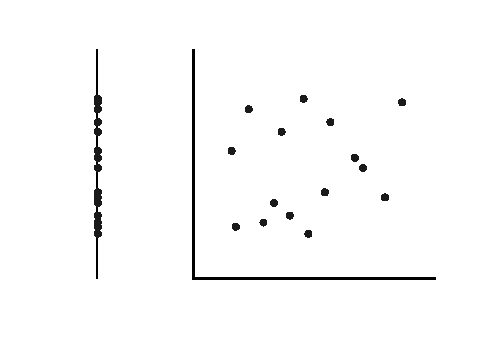
\includegraphics[width=0.6\linewidth]{Graphics/ch1/smallsample}
\caption[Illustration of one and two-dimensional spaces.]{Illustration of the separation between points in one-dimensional and two-dimensional spaces.}
\label{fig:smallsample}
\end{figure}


\section{The Small Sample Size Problem}\label{sec:smallsamplesize}
The \textit{Small Sample Size Problem} refers to a problem that arises when the proportion between number of subjects and number of features is large. Think of, \eg, 15 points in a one-dimensional line, as in Figure~\ref{fig:smallsample}. If we think of a subject as a vector, we would have 15 subjects in a one-dimensional space. Now, imagine that we add a second dimension. It is easy to see that our subjects would be farther than in the two-dimensional world. And the same would happen if we move to four, ten or thousands of dimensions. The farther our points are, the more difficult is for a statistical tool to extract information. That is what we call \textit{almost empty spaces} \cite{Duin2000,Stoeckel04}, in contrast to \textit{dense spaces}, where points are closer. 

Neuroimaging provides hundreds of thousands, or even millions of voxels, in what could mean millions of features. That implies that any calculation performed in those almost empty spaces will eventually lack information. This implies a loss of statistical power of the methods used, usually producing false negatives (the system is unable to detect real signal) and false positives (the system detects signal where there is not). These are known in statistics as Type I and Type II errors respectively. 

In differential diagnosis studies, the small sample size problem leads to wrong conclusions about where real differences are located. This, in addition to untracked confounding variables are one of the fundamental sources of non-re\-pro\-du\-ci\-bi\-li\-ty un current neuroimaging studies \cite{Button2013}. 

The solution might seem straightforward: increase sample size. But this is not always possible, since neuroimaging studies do their best at recruiting as many people as they can with a limited budget. Many efforts have been put into establishing multi-centre collaborations that allow the recruitment of a larger population, but despite offering a higher statistical power, these studies still suffer from a number of confounding variables such as population bias or scanner differences \cite{haar2014anatomical}. In chapters~\ref{ch:swpca} and \ref{ch:simulation} we explore different approaches to this solution. 

Another option involves reducing the number of features, via feature selection or feature extraction. This has been widely used in computed-aided methodology for neuroimaging \cite{DeMartino2007,Xu2009,Gorriz2010,Illan2011,Martinez-Murcia2016} with great success, and solutions using this approach will be treated in chapters~\ref{ch:decomposition}, \ref{ch:texture} and \ref{ch:sbm}. 

The Small Sample Size problem is directly related to the \textit{Curse of Dimensionality} \cite{Krishnaiah1982}, which proves that, in contrast to what could be expected, once a certain classifier performance has been achieved, it holds or even decreases when feeding more features to the classifier. The problem also affects statistical hypothesis testing, a tool widely used for inference in neuroimaging, in what is known as the \textit{Multiple Comparisons} problem \cite{Benjamini2010}, a particular field that is still being studied. 

\section{Aims and Objectives}\label{sec:overview}
This thesis aims to contribute new approaches to overcome the small sample size problem in neuroimaging. This can provide more accurate \ac{CAD} systems by reducing the number of false positives, increasing the reliability of their results. 

We will take two different approaches, as commented in previous sections: increasing the sample size and reducing the feature space. Therefore, we can define the following objectives: 

\begin{itemize}
	\item Develop and evaluate algorithms that reduce the feature space, in which is usually known in the field as feature extraction and feature selection strategies. 
	\item Develop and evaluate new strategies to increase the sample size in neuroimaging studies. 
\end{itemize}

Most of the studies in the literature focus on the first objective. Feature extraction algorithms that use \ac{PCA} \cite{Khedher2015,Towey2011} or Partial Least Squares \cite{Segovia2013}, among others, are widely studied. We have developed three different approaches to those:

\begin{itemize}
	\item A combination of image decomposition algorithms and feature selection. In this approach we have used three criteria to select the most significant voxels from the images, and then applied \acf{FA} and \acf{ICA} to decompose the data and significantly reduce their feature space. 
	\item A feature extraction based on texture analysis. 
	\item A novel strategy called \acf{SBM}. This feature extraction technique uses a spherical coordinate system to map statistical measures to a bidimensional plane. It builds paths used as feature selection vectors where several measures are computed. 
\end{itemize}

On the other hand, we have evaluate newer ways to increase sample size in neuroimaging studies. We have developed: 
 \begin{itemize}
 	\item A system to reduce undesired variance in structural multicentre studies, called \acf{SWPCA}. This system is intended to reduce the amount of false positives in large collaborations, providing more homogeneous images and improving their statistical analysis. 
 	\item An algorithm to simulate functional brain images using existing data, and therefore, increase sample size. 
 \end{itemize}

\begin{figure}
	\centering
	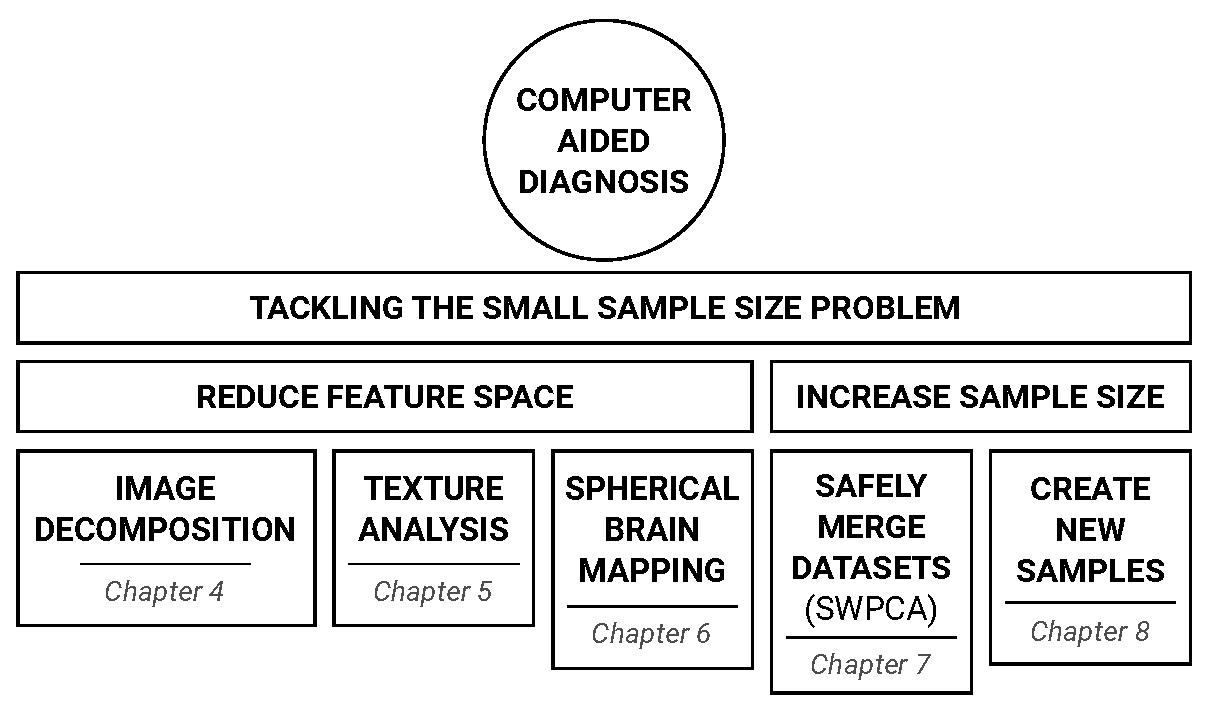
\includegraphics[width=0.7\linewidth]{Graphics/ch1/outline}
	\caption[Structure of the thesis.]{Structure and connexions between the different strategies proposed in this thesis, organized by chapters and parts.}
	\label{fig:outline}
\end{figure}


\section{Organization of this Thesis}
This thesis work is organized in four parts plus appendices, each of which is subdivided in several chapters. In the first part, we introduce the motivations and main aims of this work (chapter~\ref{ch:introduction}), examine the state of the art in medicine, neuroimaging and \ac{CAD} systems (chapter~\ref{ch:stateofart}) and present a general methodology that will be followed throughout this thesis, including preprocessing and evaluation (chapter~\ref{ch:preprocessing}). 

Parts \ref{part:feature} and \ref{part:increase} refers to each of the solutions outlined in the previous section, and disaggregated in Figure~\ref{fig:outline}. In part~\ref{part:feature} we focus on the feature reduction techniques, including decomposition methods (chapter~\ref{ch:decomposition}), texture analysis (chapter~\ref{ch:texture}), and the novel algorithm Spherical Brain Mapping (chapter~\ref{ch:sbm}). On the other hand, Part~\ref{part:increase} is focused on two different strategies used to increase the sample size: the Significance Weighted Principal Component Analysis algorithm (chapter~\ref{ch:swpca}), used to safely merge structural images acquired at different centres, and a neuroimage simulation algorithm (chapter~\ref{ch:simulation}) that can be used to extend existing functional datasets. 

Finally, in Part~\ref{part:dicussion} we provide a general discussion of the results presented in this thesis, conclusions about the methods and prospective work that could be performed with this basis. 

\section{Contributions}
Some ideas and figures have appeared previously in the following publications, that we divide here in articles and conference presentations. 

%\noindent Put your publications from the thesis here. The packages \texttt{multibib} or \texttt{bibtopic} etc. can be used to handle multiple different bibliographies in your document.

\begin{refsection}[ownpubs]
	\small
	\nocite{*} % is local to to the enclosing refsection
	\newrefcontext[sorting=ydnt]
	\subsection{Articles}
	\printbibliography[env=nolabelbib,heading=none,keyword=own, title={Articles}, type=article]
	\subsection{Conferences}
	\printbibliography[env=nolabelbib,heading=none,keyword=own, title={Conferences}, type=inproceedings]
	\subsection{Books}
	\printbibliography[env=nolabelbib,heading=none,keyword=own, title={Books}, type=inbook]
\end{refsection}


% DONE
%*****************************************
\chapter{State of the Art}\label{ch:stateofart}
%*****************************************
In this chapter, after an introduction to the neurological and psychiatric disorders treated in this thesis, in Section~\ref{sec:disorders}, we will explore neuroimaging modalities in Section~\ref{sec:neuroimaging}, the state-of-the-art voxel-wise analyses used in the neuroimaging community at Section~\ref{sec:vwanalyses} and recent contributions to the field using Machine Learning. 

\section{Diseases and Disorders}\label{sec:disorders}
First of all, it is interesting to provide some medical background about the diseases that we have applied or methodology to. This is the case of \ac{AD}, \ac{PKS} and \ac{ASD}. In this chapter, we will explore what we currently know about causes, symptoms and particularities of these diseases, and how these can be identified using neuroimaging. 


\subsection{Alzheimer's Disease}
\ac{AD} is whatever.. 

% Alzheimer
Alzheimer's Disease (AD) is currently the most common neurodegenerative disease in the world, with more than 44.4 million affected people, and it is likely to have increased up to 135.5 million by 2050. According to research, most people currently living with this type of dementia have not received a formal diagnosis \cite{ADInforme2013}. In this task, the development of medical imaging has represented a major breakthrough, allowing the physicians to explore a number of structural and functional biomarkers that previously could only be accessed post-mortem. 

Recently, a number of very specific radiopharmaceuticals, such as Pittsburgh compound B (PiB), a radioactive analog of thioflavin T that  binds to fibrillar amyloid-beta (A$\beta$), have been developed. However,  their invasive nature and their technical requirements -specially when the half-life of the radioactive element is usually low, and therefore, its synthesis requires a nearby cyclotron- make them unusual in the clinical practice. Conversely, Magnetic Resonance Imaging (MRI) is a more widespread technique that allows the characterization of brain atrophy, and accordingly, is far more established in clinical practice. 


Wikipedia: The cause of Alzheimer's disease is poorly understood [1]. About 70\% of the risk is believed to be genetic with many genes usually involved.[6] Other risk factors include a history of head injuries, depression, or hypertension.[1] The disease process is associated with plaques and tangles in the brain.[6] A probable diagnosis is based on the history of the illness and cognitive testing with medical imaging and blood tests to rule out other possible causes.[7] Initial symptoms are often mistaken for normal ageing.[1] Examination of brain tissue is needed for a definite diagnosis.[6] Mental and physical exercise, and avoiding obesity may decrease the risk of AD.[6] There are no medications or supplements that decrease risk.[8]

TEsts

Therefore, MR brain images have been extensively used in the diagnosis of AD by assessing neurodegeneration on grey matter (GM) and White Matter (WM) tissues. Research has shown in \cite{Baron2001,Misra2009,Pievani2013,Dubois2007} that neurodegeneration in Alzheimer's Disease mainly occurs in the GM tissue. Particularly grey matter loss has been described in the Hippocampus and Parahippocampal lobes, according to the NINCDS-ADRDA criteria for AD diagnosis \cite{Dubois2007}, with further atrophy described in the medial temporal structures, the Posterior Cingulate gyrus and adjacent Precuneus \cite{Baron2001}. Moreover, significantly lower volumes of certain regions in GM and WM have been considered a promising biomarker and predictor of the progression of AD in a longitudinal study involving Mild Cognitive Impairment (MCI) patients \cite{Misra2009}, and some structures in the striatum (putamen and caudate nucleus) have shown important volume abnormalities \cite{Pievani2013}. All these data suggest that many of the symptoms of AD can be observed in anatomical MR images even in early stages of the disease, which could be of great help in its successful diagnosis and treatment. 

Specifically, it highlights the posterior cingulate gyri and precunei, as well as the temporo-parietal region, both considered as typically affected by glucose hypometabolism in the AD \cite{Claus1994}.

En la enfermedad de Alzheimer, regiones característi-
cas muestran un decrecimiento en el metabolismo de glucosa, específicamente
regiones bilaterales en los lóbulos temporal y parietal, cíngulo posterior y pre-
cunei y también en el cortex frontal y el conjunto global del cerebro en casos
de afección severa (de Leóon et al., 1983; Foster et al., 1983, 1984; Chase et
al., 1984; Duara et al., 1986; McGeer et al., 1990; Minoshima et al., 1994,
1995; Ibañez et al., 1998; Hoffman et al., 2000; Kogure et al., 2000; Alexan-
der et al., 2002; Mosconi et al., 2008; Langbaum et al., 2009).


\subsection{Parkinsonism}
Parkinsonian Syndrome (PS), also known as Parkinsonism, is a neurological syndrome characterized by tremor, hypokinesia, rigidity and postural instability \cite{Eckert2007}. It is considered as the second most common neurodegenerative disease, with a prevalence of 1-3\% in the population over 65 years of age \cite{Moghal1994}. A wide range of etiologies may lead to the PS, while the most common cause is the neurodegenerative condition called Parkinson's Disease (PD). This disease originates due to the progressive loss of dopaminergic neurons of the nigrostriatal pathway, which connects the substantia nigra to the striatum. As a result, the dopamine content of the striatum decreases, and consequently, dopamine transporters (DAT) are lost. Other possible causes include  some toxins, a few metabolic diseases, and a handful of non-PD neurological conditions (atypical parkinsonian syndromes), such as multiple system athropy (MSA), progressive supranuclear palsy (PSP) or corticobasal degeneration (CBD) \cite{Christine2004,tatsch2008extrapyramidal}. 

% DaTSCAN images
\subsubsection{Parkinson's Disease}
As the PD is related to a loss of dopamine transporters in the nigrostriatal pathway, the study of its status by means of brain imaging techniques has set a breakthrough in the diagnosis process, particularly in the  case of parkinsonian syndromes \cite{Eckert2007,Scherfler2009,Bhidayasiri2006}. $^{123}$I-ioflupane (best known by its trade name DaTSCAN) is a tracer derived from cocaine analogue, which binds to the dopamine transporters in the striatum \cite{Booij1998,Winogrodzka2003}. Then, the density of these transporters is measured using Single Photon Emission Computed Tomography (SPECT). As a result, images show a reduced uptake of the tracer in the striatum in patients with PS \cite{Bhidayasiri2006,PunalRioboo2007}. 
\subsubsection{Extrapyramidal Symptoms}
\subsection{Autism Spectrum Disorder}
Autism Spectrum Disorder (ASD) is a neurodevelopmental syndrome characterized by social and communication impairment as well as restricted, repetitive patterns of behaviour, interests or activities. The delimitation of both functionally and structurally affected areas in the brain in such an etiologically and neurobiologically heterogeneous condition has long been a major concern (Ecker and Murphy, 2014; Lai, et al., 2013; Lenroot and Yeung, 2013). With this context, the use of large samples is of fundamental importance, and has been addressed by establishing multi-centre collaborations such as the UK Medical Research Council Autism Imaging Multi-centre Study (MRC AIMS) (Ecker, et al., 2013; Ecker, et al., 2012) and the Autism Brain Imaging Data Exchange (ABIDE) (Di Martino, et al., 2014).


\section{Neuroimaging Modalities}\label{sec:neuroimaging}
Medical imaging refers to all types of 2D, 3D and 4D images used in clinical practice. These involve many different modalities, among them X-rays, ultrasound, endoscopy, microscopy, etc. In neuroimaging, the most extended is by far \ac{MRI}, which provides intensity maps that represent the internal structure of the brain. Other modalities are aimed at studying the function of the brain, by injecting radioactive ligands that, linked to a receptor, can measure its distribution. This is the case of \ac{PET} and \ac{SPECT}.

\subsection{Magnetic Resonance Imaging}
\acf{MRI} is perhaps the most widespread in neuroimaging, given its ability to visualize both structural and functional (in functional \ac{MRI}) properties of the brain, and, in contrast to other imaging modalities, is considered non-invasive. \ac{MRI} uses strong magnetic fields to excite certain atomic nuclei, that can absorb and emit this energy. 

\begin{figure}[htp]
	\centering
	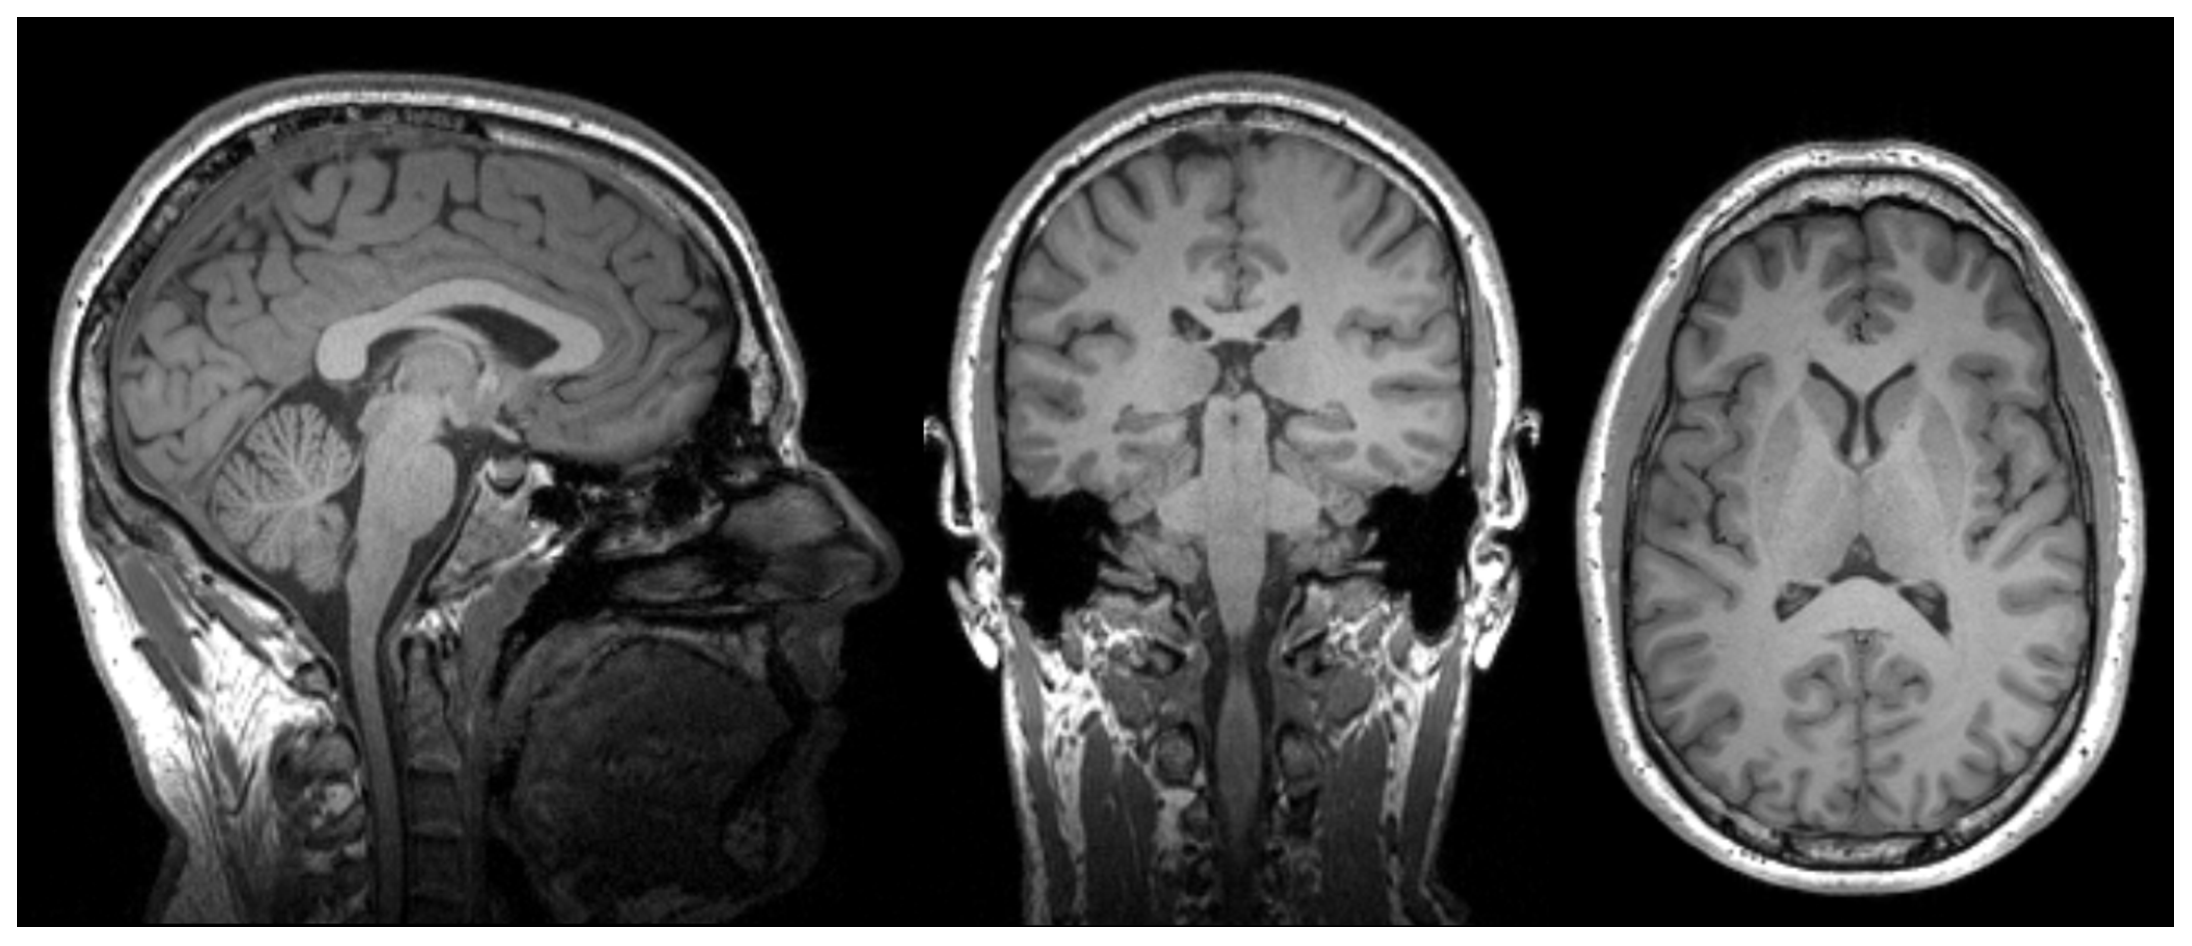
\includegraphics[width=0.7\linewidth]{Graphics/ch1/example_MRIT1}\\
	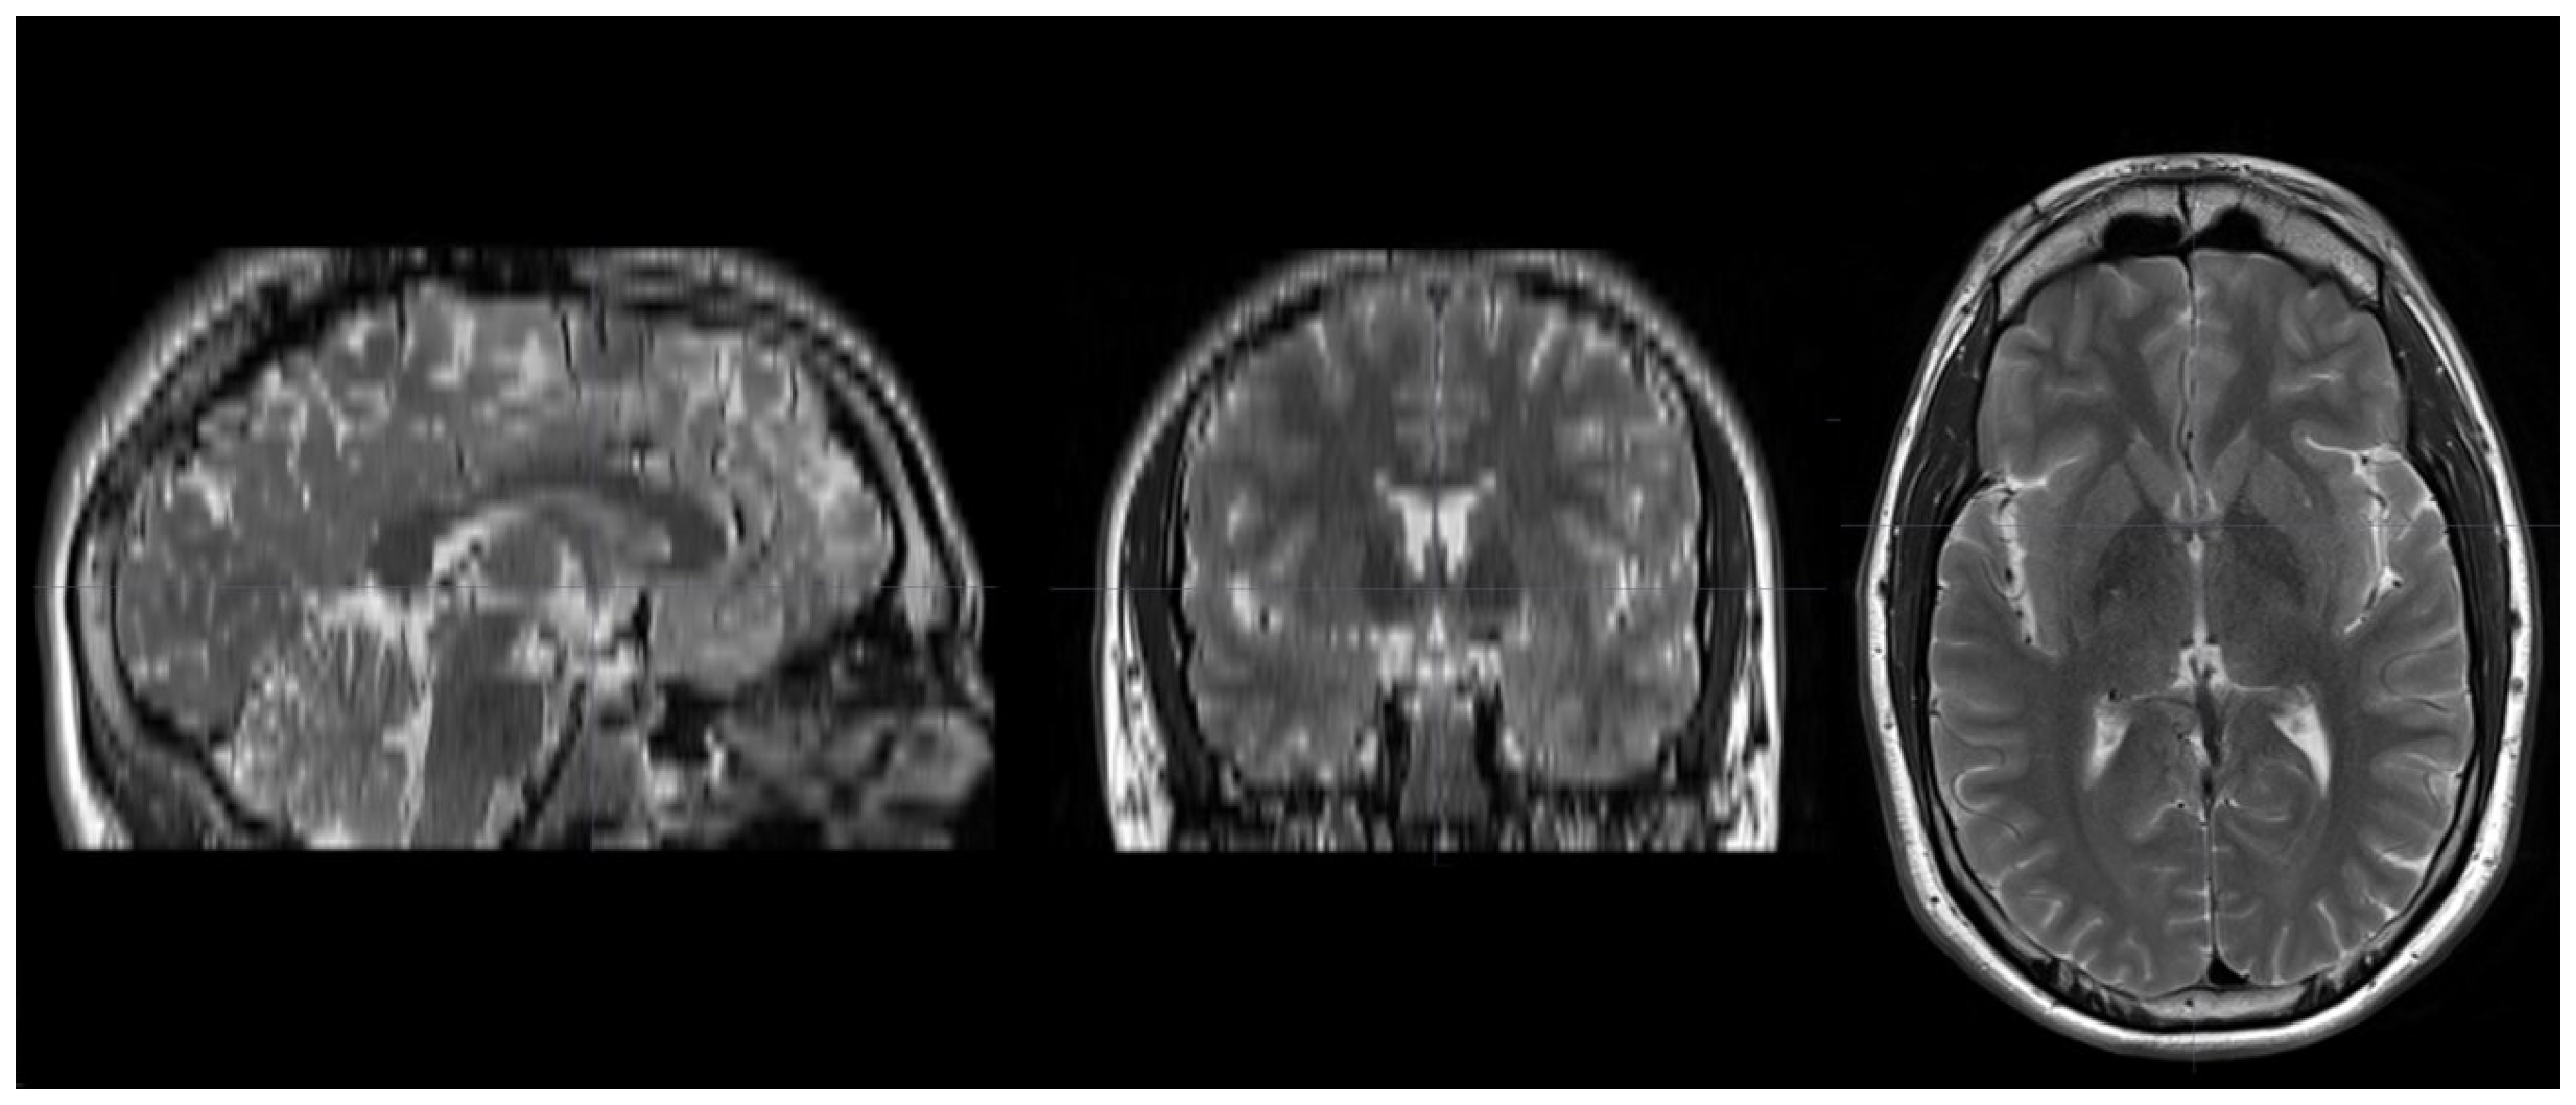
\includegraphics[width=0.7\linewidth]{Graphics/ch1/example_MRIT2}
	\caption[Example of T1 and T2-weighted MRI images.]{Example of T1 and T2-weighted MRI images of the same subject.}
	\label{fig:example_MRI}
\end{figure}

\ac{MRI} combines the magnetic field with a \ac{RF} emission to excite the atomic nuclei present in corporal structure, resulting in a image of the distribution of certain atoms in the body. Most \ac{MRI} use hydrogen atoms, since they are present in water (which adds up to around 70\% of body mass) and the signal derived is stronger than other atoms, increasing the \ac{SNR}, and therefore, the image quality. 

The procedure uses a strong magnetic field $B_0$ to align the magnetic moment of the hydrogen nuclei in parallel or anti-parallel (depending of their initial spin). This way, the magnetic moment of all nuclei will increase up to a stable state, in contrast to their null value in absence of $B_0$. Within this magnetic field, the hydrogen atoms precess around an axis along the direction of the field. 

A given nuclei has a resonance frequency which is proportional to the intensity of $B_0$, which, by using strong fields, allow us to resonate hydrogen far below potentially damaging frequencies. The precession frequency is determined by the Larmor equation (\ref{eq:lamor}):

\begin{equation}\label{eq:lamor}
f_0 = \frac{\gamma}{2\pi } B_0 
\end{equation}
where $\gamma$ depends on the nuclei, which in the case of hydrogen, $\gamma = 42.6$ MHz/T. When a subject is introduced in the \ac{MRI} scanner, it is submitted to the magnetic field $B_0$, so that the hydrogen nuclei are aligned to the field, with a precession frequency $f_0$. Then, a \ac{RF} pulse of the same frequency is generated, which is then absorbed by the nuclei, forcing them to place perpendicular to the field. Once the \ac{RF} emission is interrupted, the nuclei return to its equilibrium state by means of a procedure called relaxation. In this procedure, they emit part of the absorbed energy, which is then captured by a \ac{RF} receptor. Usually, position information is encoded in the \ac{RF} signal by varying $B_0$ using gradient coils. 

The \ac{RF} signal is measured during the relaxation time, and two different relaxation times are set: the T1 (spin-lattice) relaxation time and the T2 (spin-spin) relaxation time. The T1 time is the time during which nuclei emit energy to the adjacent tissue and realign to the longitudinal plane (z axis), whereas the T2 time refers to the time when nuclei realign to the transversal plane (y axis). These times are used to create T1-weighted and T2-weighted images (see Figure~\ref{fig:example_MRI}). T1-weighted images allow to distinguish between \ac{GM} and \ac{WM} in the cerebral cortex, to identify fatty tissue, and generally, obtain structural information. Conversely, T2-weighed images are used to assess \ac{CSF} or to visualize and identify \ac{WM} lessions. 

\subsection{Single Photon Emission Computed Tomography}
The \acf{SPECT} is based on the principles of \ac{CT}, by which a series of signal acquisition at different angles can be reconstructed back into a bidimensional distribution of the signal. In \ac{SPECT}, a gamma photon emitting radioisotope is linked to a pharmaceutical that binds to a given biomarker, generating a radiopharmaecutical or agent. This agent is injected into the patient, and after a certain time in which the radiopharmaceutical is distributed, the patient is introduced into the \ac{SPECT}-\ac{CT} scan. 

Afterwards, the scanner performs a series of acquisitions at different planes and angles from the body, from which the gamma signal is measured. For each plane, all acquisitions at each angle are pooled and a single two-dimensional image is reconstructed using a \ac{FBP} algorithm, or Radon inversion formula \cite{Herman2009l}, which derives from the Fourier's Theorem. A total of 180 projections per plane, using an angular resolution of 2 degrees, are usually taken. 

There exist a number of radiopharmaceutical used in clinical practice, and therefore, we will focus on the two varieties used in this thesis. First, we use an agent called $^{99m}$Tc-HMPAO, which consists of two stereoisomers of hexametazime (HMPAO) linked to the radioisotope technetium 99-metastable. This agent is usually used to assess \ac{rCBF}, which can be used to diagnose neurological diseases or cancer. 

\begin{figure}[htp]
	\centering
	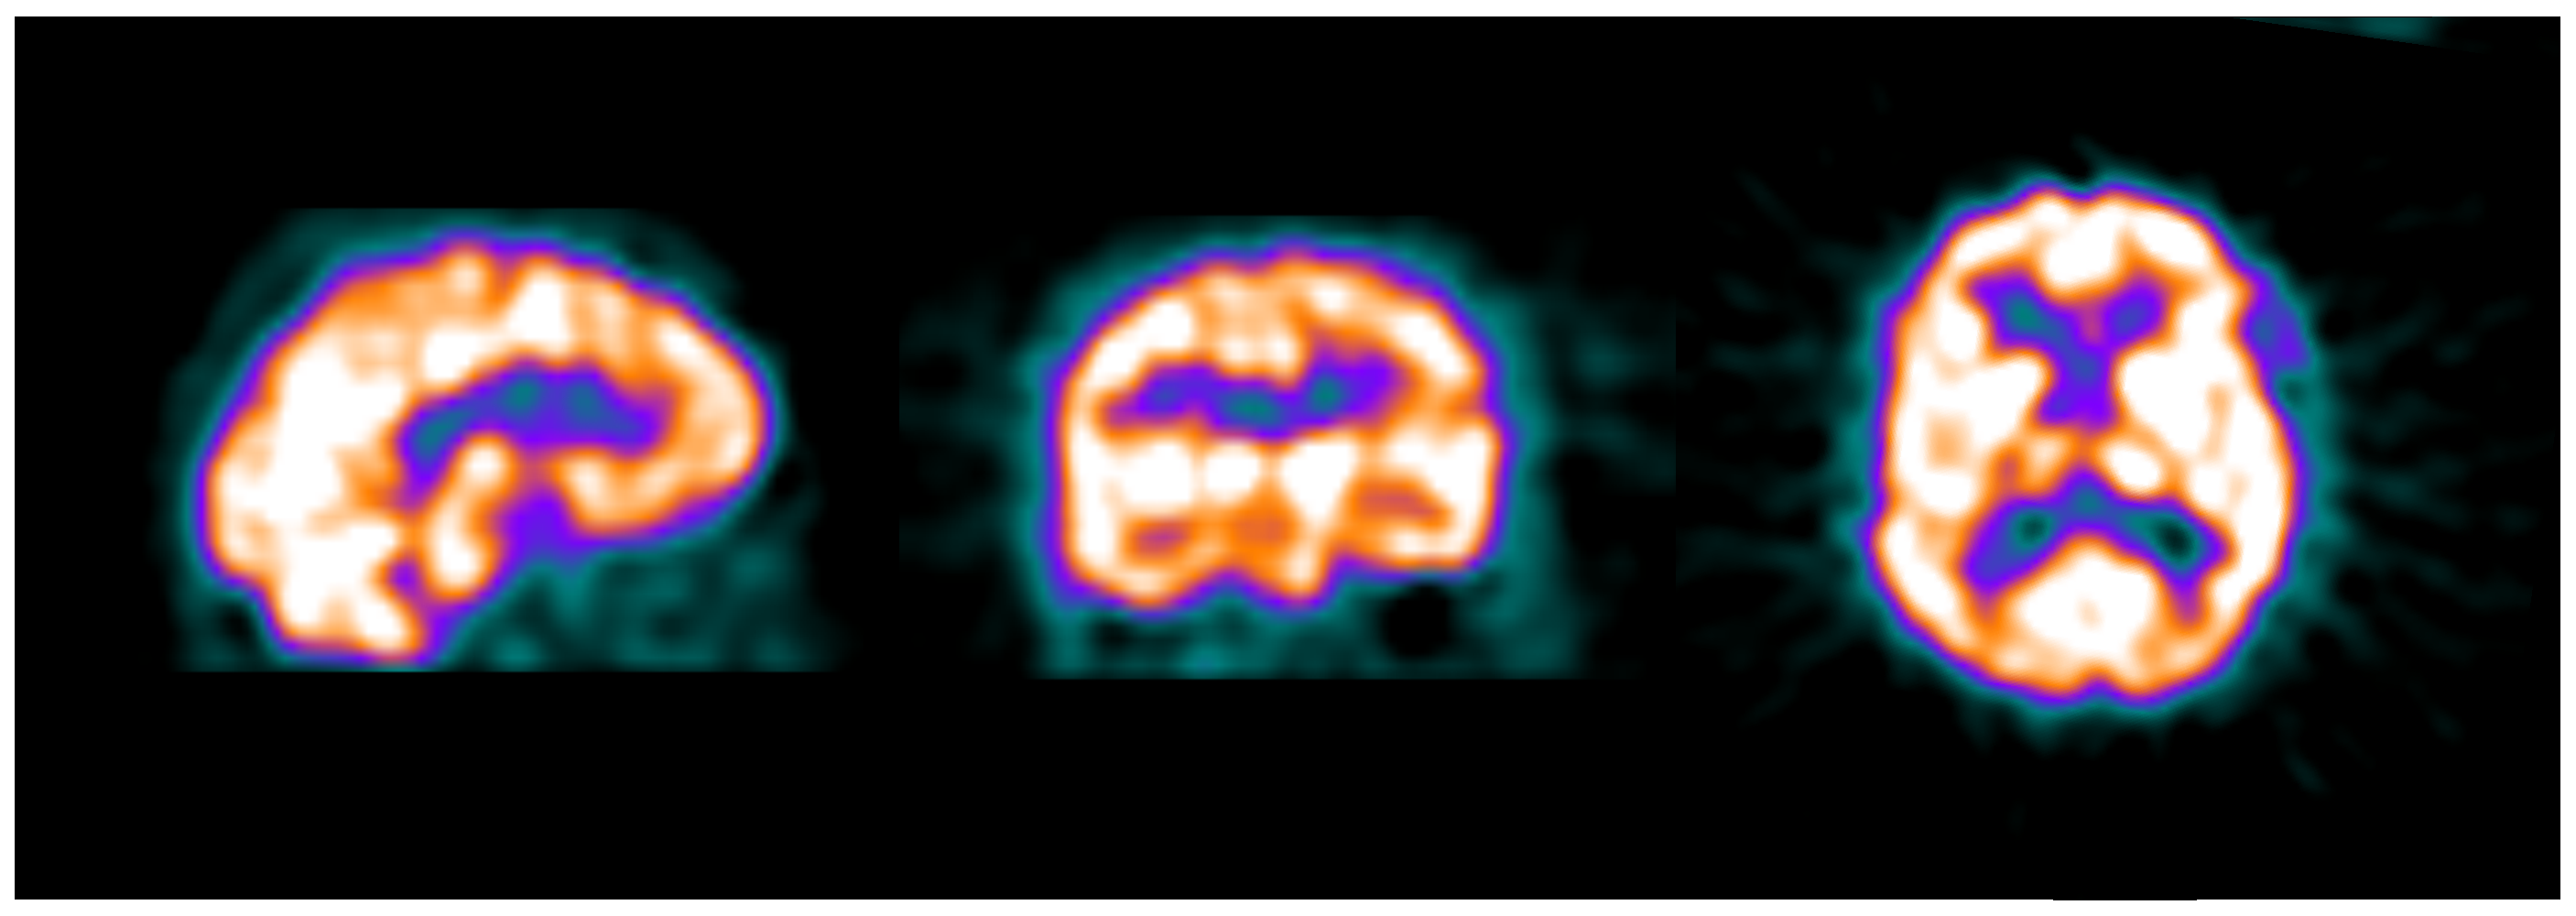
\includegraphics[width=0.7\linewidth]{Graphics/ch1/example_SPECT}\\
	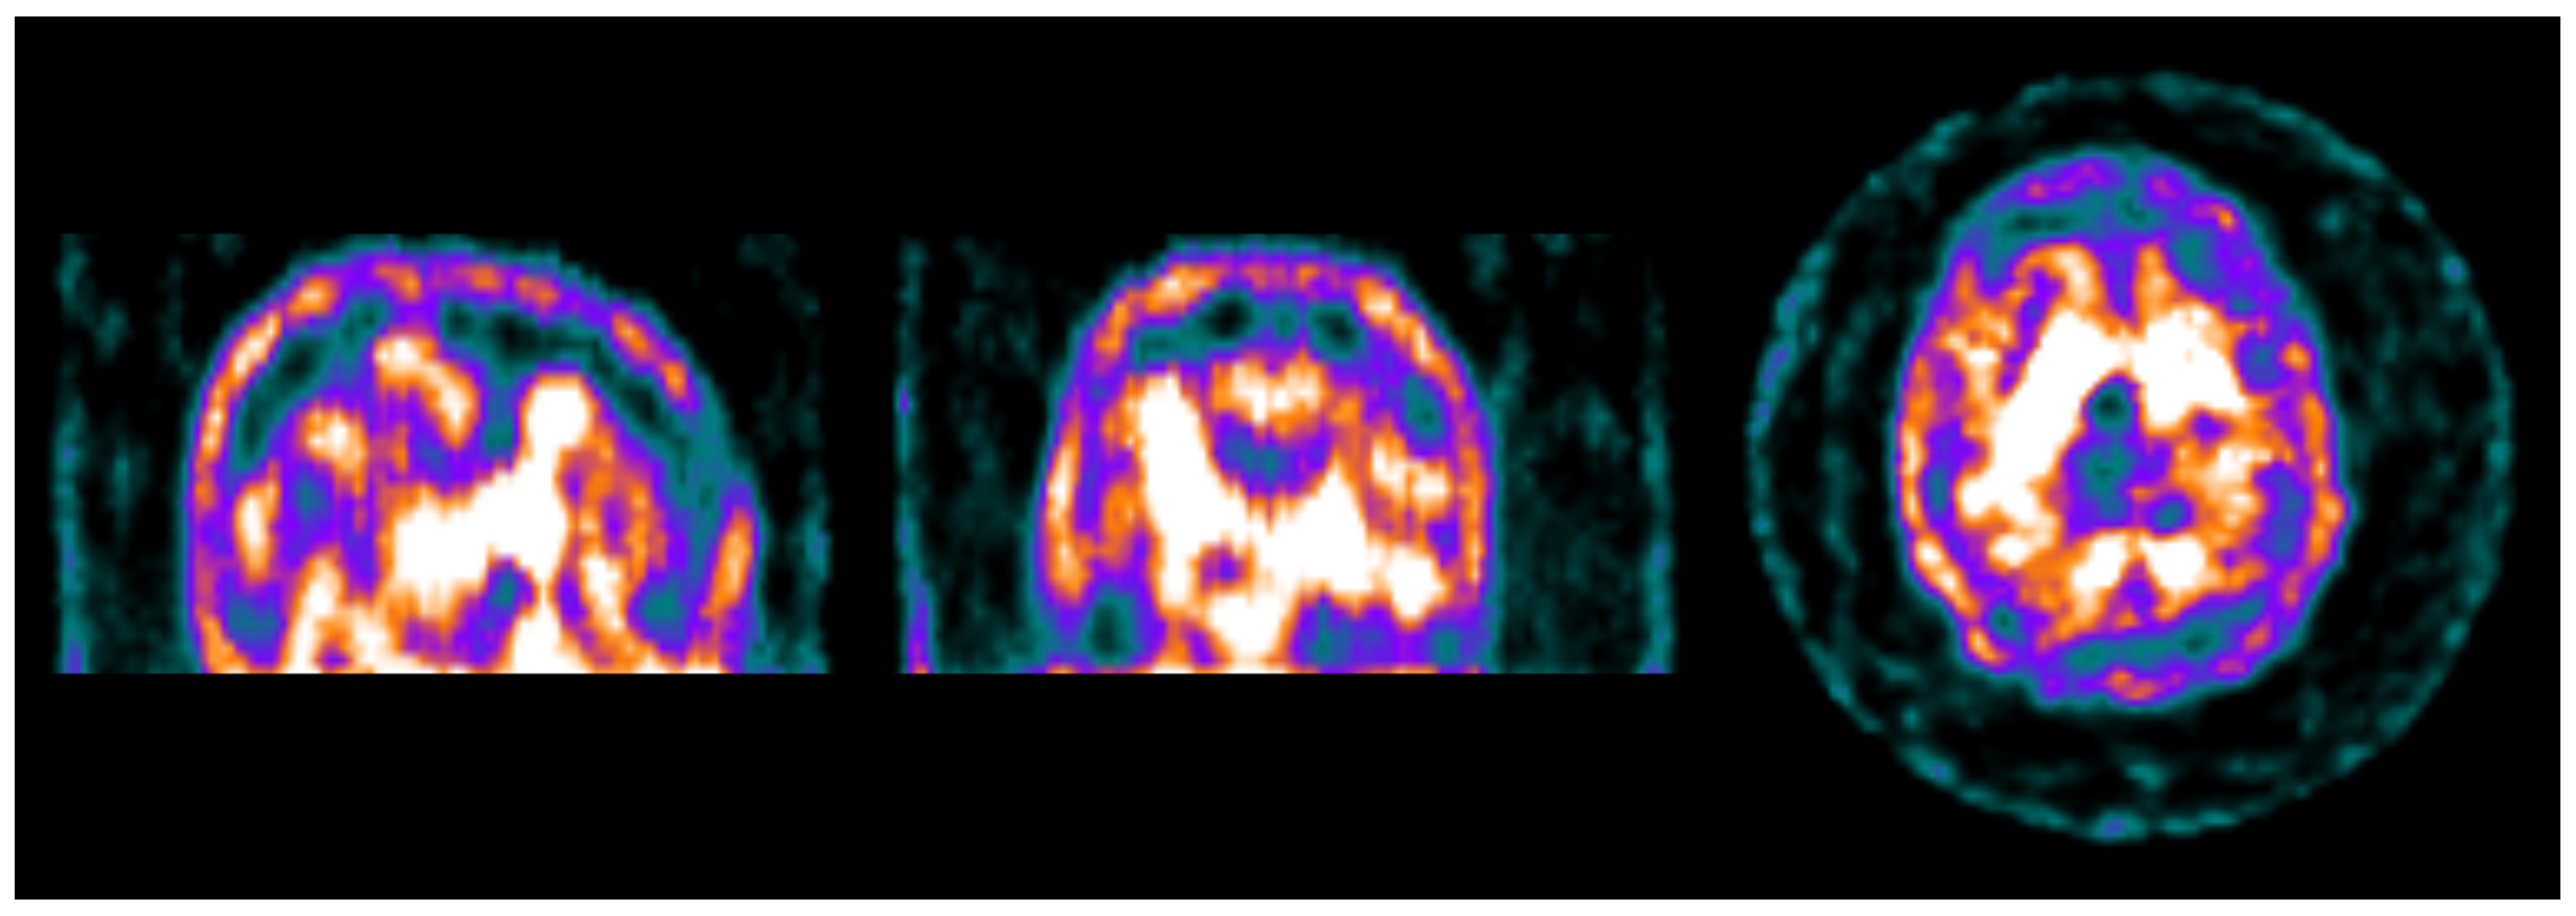
\includegraphics[width=0.7\linewidth]{Graphics/ch1/example_DaTSCAN}
	\caption[Example of SPECT images.]{Example of SPECT images, a SPECT-HMPAO and a SPECT-DaTSCAN.}
	\label{fig:example_SPECT}
\end{figure}

Additionally, we use images generated using the agent Ioflupane ($^{123}$I), a cocaine analog with high binding affinity for \ac{DAT}. It is used fundamentally in the assessment of \ac{PD}, given that the disease is associated with a loss of dopaminergic neurons in the striatal region. 

\subsection{Positron Emission Tomography}
The \acf{PET} is a technique similar to \ac{SPECT}, but in this case, the agent used and the equipment is designed to deal with a pair of gamma photons resulting of the annihilation of a positron with its corresponding antiparticle, the electron. The pair of photons are generated in opposite directions, and the detection depends on them being simultaneously or coincidently detected at the receptor. The receptor comprises a scintillator which emits light when the gamma photon incides, and a detector, usually a photomultiplier tube or silicon avalanche photodiodes.

It uses the same \ac{FBP} algorithm as \ac{SPECT} in the reconstruction of the images, and a similar strategy for acquiring the signal at different angles. However, the amount of data is smaller than in \ac{SPECT}, and therefore, the reconstruction procedure is harder. As a result, \ac{PET} scanner operation is considered more costly than \ac{SPECT} \cite{Carlson2016}.  

\begin{figure}[htp]
	\centering
	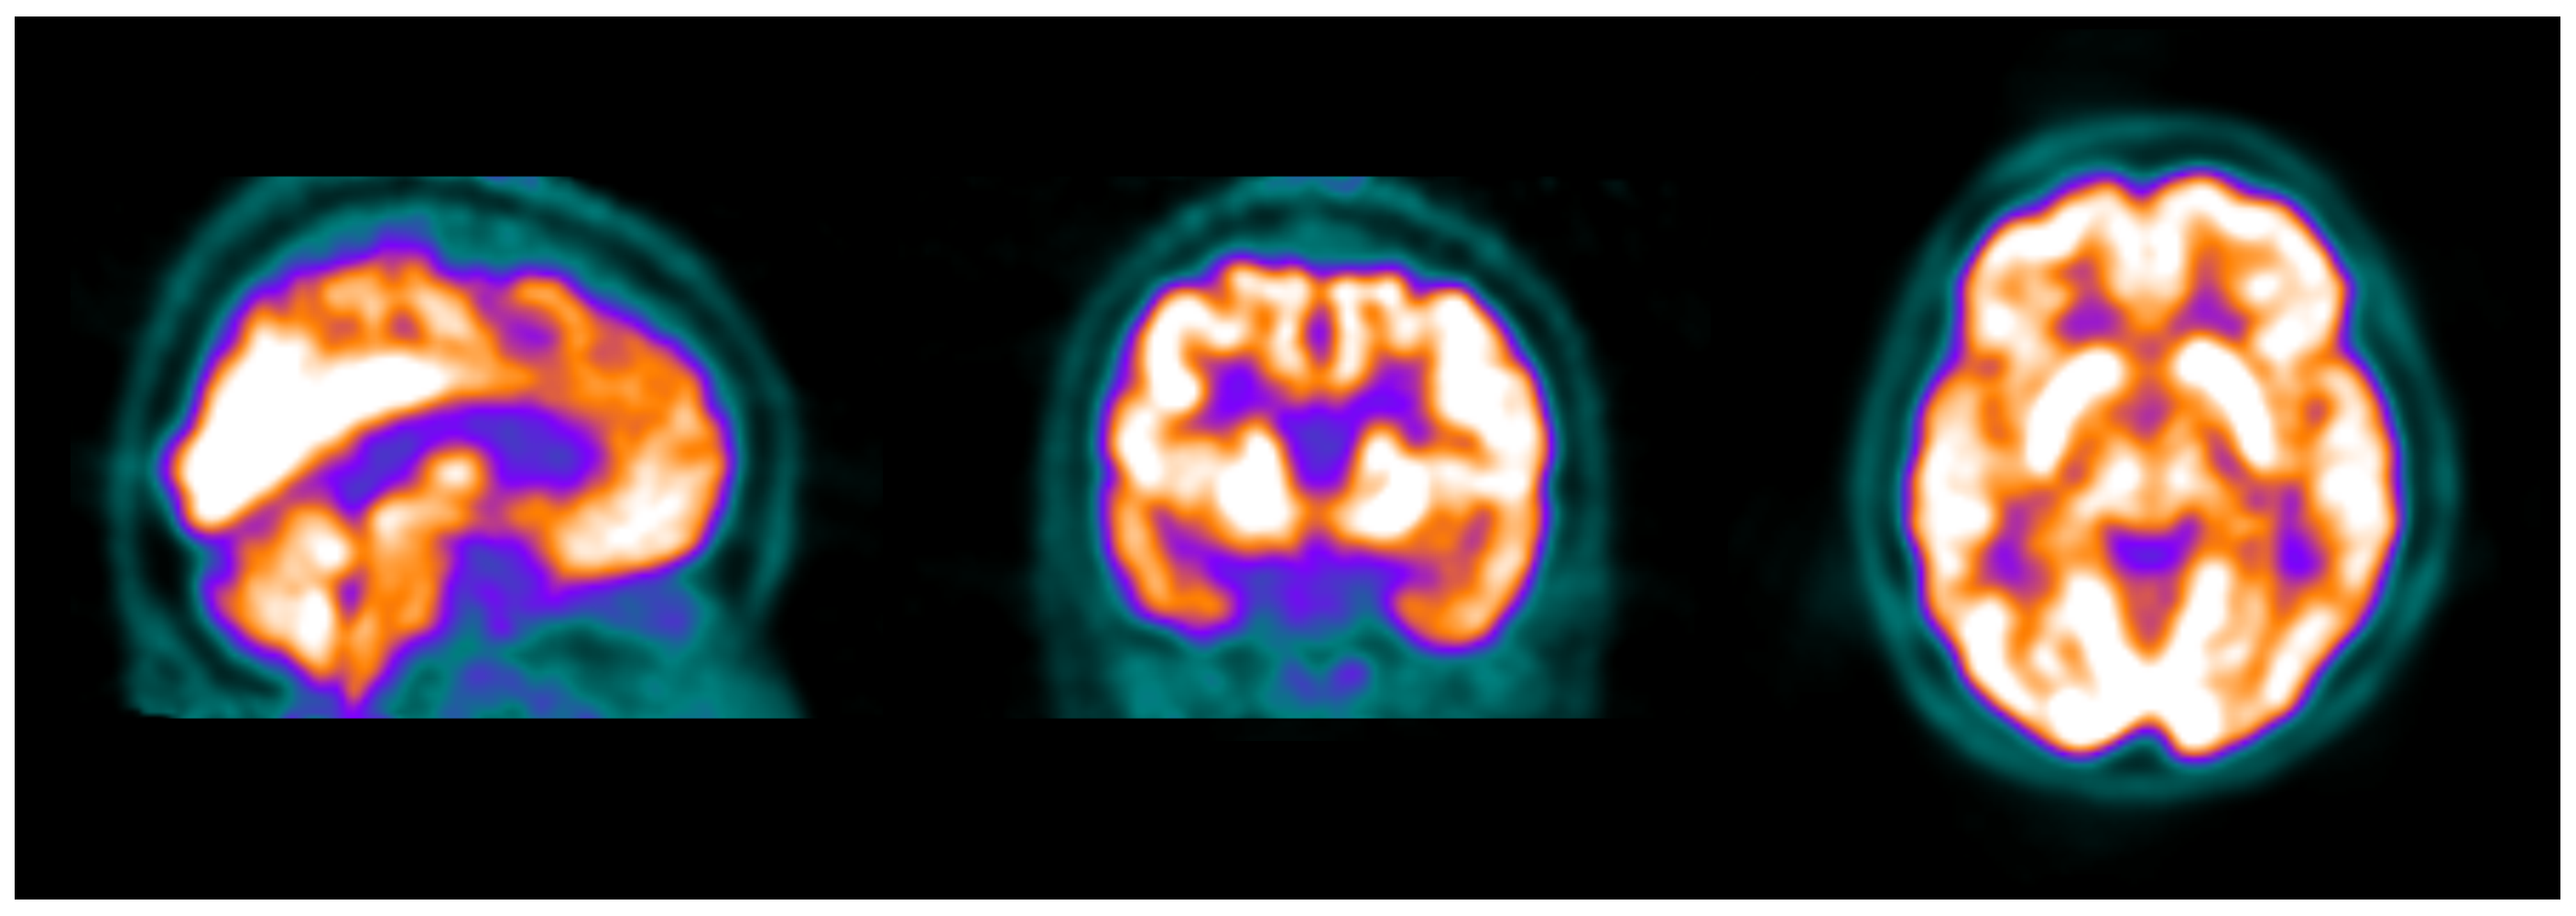
\includegraphics[width=0.7\linewidth]{Graphics/ch1/example_PET}
	\caption[Example of a PET-FDG image.]{Example of a PET-FDG image.}
	\label{fig:example_PET}
\end{figure}

The agent used in the images that we have processed is PET-FDG, also known as Fludeoxyglucose ($^{18}$F). It is a glucose analogue that allows us to measure the glucose metabolism in the brain. It is widely used in neurology \cite{Newberg2002} and cancer detection \cite{Kelloff2005}, since it can be correlated with cellular activity. 


\section{Voxelwise Analyses}
Traditional analysis of neuroimaging involves visual analysis by experts clinicians, or semi-quantitative analysis of \acp{ROI}. With the rise of neuroimaging in the mid-nineties, some computer-aided solutions appeared, starting with the widely known \acf{SPM} \cite{Friston1994}, its extension to structural imaging \acf{VBM} \cite{Ashburner2000} and later, the first application of classifiers to medical imaging, called \acf{VAF} \cite{Stoeckel04}.

\subsection{Statistical Parametric Mapping}
\acf{SPM} is a new methodology to automatically examine differences in brain activity in functional imaging studies involving \ac{fMRI} or \ac{PET}, firstly proposed by Friston in \cite{Friston1994}. The technique can be applied either to static images (e.g., \ac{PET}) or timeseries (\ac{fMRI}), using inference techniques based on hypothesis testing, in order to construct the \ac{GLM} that better describes the variability in the data. 

Statistical hypothesis testing involves constructing a pair of hypotheses: $H_0$, or the null hypothesis, that states no relationship between variables; and $H_1$, the alternative hypothesis. In neuroimaging, $H_0$ usually means that there are no relevant differences between classes (for example, between patients affected by \acf{AD} and \ac{CTL}), and $H_1$ implies that there is a significant difference. Many different tests such as massive univariate $t$-Test or \ac{ANOVA} (see Chapter~\ref{ch:decomposition} for more information on these techniques) can be used in the \ac{SPM} software \cite{spm_book}, by using a design matrix that describes a $t$ or $F$ based contrast (for $t$-Test and \ac{ANOVA} respectively). These terms are generally referred to as $Z$-values, namely the signed number of standard deviations an observation is above the mean. 

The test are computed voxel-wise, from which a $p$-value can be obtained, nominally the probability of obtaining equally or more extreme $Z$ values that the one actually found.
$p$-values are very extended in neuroimaging, representing the probability of a $Z$ value being equal or more extreme than the reference value given. In many studies $p < 0.05$ is used for measuring statistical significance, which means that only a 5\% of the times a experiment is repeated we would obtain that result or a more extreme one. The use of the significance threshold $\alpha=0.05$ implies that any voxel with a $p$-value smaller than 0.05 is considered sufficient to reject the null hypothesis. 

\begin{figure}[htp]
	\centering
	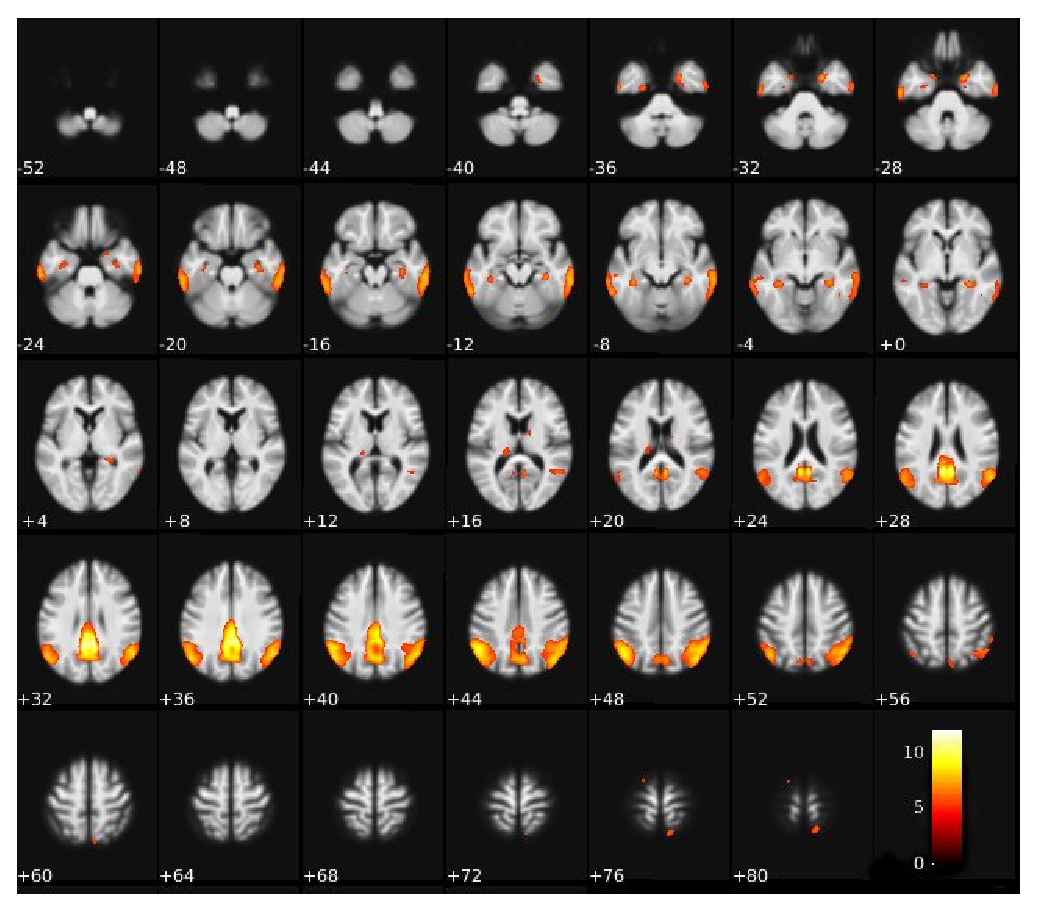
\includegraphics[width=\linewidth]{Graphics/ch1/example_SPM}
	\caption[Example of a \acs{SPM} analysis on a \acs{PET} dataset.]{Example of a \ac{SPM} analysis on a \ac{PET} dataset displaying the differences between \ac{AD} and \ac{CTL}, using $p<0.05$ and \ac{FWE} correction.}
	\label{fig:example_SPM}
\end{figure}

\ac{SPM} outputs maps like the one shown in Figure~\ref{fig:example_SPM}. There, significant $Z$-values according to a given threshold (\ac{FWE} uncorrected or corrected, see Section~\ref{sec:multiplecomparisons}) are displayed over an anatomical reference.  The resulting maps allow a visual inspection of the active brain areas, which can later be related to a certain disease or task. 

Although \ac{SPM}'s main feature is the estimation of differences, the term has been extended to cover the whole process performed by the \ac{SPM} software. That is, it generally involves registration to a template, intensity normalization, smoothing, the proper \ac{SPM} difference estimation and the display of the results. An overview of these procedures is provided at Chapter~\ref{ch:preprocessing}. 

\subsection{Voxel Based Morphometry}
\acf{VBM} can be considered an extention of \ac{SPM} applied to structural \ac{MRI} images \cite{Ashburner2000}. The procedure involves preprocessing (see Chapter~\ref{ch:preprocessing}), where smoothing is applied to reduce smaller anatomical differences. Afterwards, a \ac{GLM} is applied to each voxel in the images, and a $Z$-score map similar to Figure~\ref{fig:example_SPM} is produced. 

Smoothing is more important in \ac{VBM} than in regular \ac{SPM}, since \ac{MRI} images have higher resolution and are less noisy than functional images. Larger smoothing kernels will miss out smaller regions, while smaller kernel can lead to artifacts in the generated $Z$-maps, including misalignment of brain structures, differences in folding patterns or misclassification of tissue types \cite{Martinez-Murcia2016book}. Therefore, the kernel size must be carefully chosen, usually using a-priori knowledge about the regions affected, and always double checking for artifacts and reproducibility. 

The idea behind \ac{VBM} has been extended in a number of papers, using multivariate approaches that takes into account all voxels at once, and not their individual differences. Some of them include \ac{ICA} decomposition of the dataset and a posterior conversion to $Z$-scores in what was called Source Based Morphometry \cite{xu2009source}, or multidimensional Tensor Based Morphometry \cite{bossa2010tensor}. 
\subsection{The Multiple Comparisons Problem}\label{sec:multiplecomparisons}
The Multiple Comparisons problem arises when using hypothesis testing to assess statistical significance. This is widely used in neuroimaging, where statistical tests such as the $t$-Test or \ac{ANOVA} are used to quantify voxel-wise differences, and state their statistical significance, or $p$-value. The $p$-value, as described above, is the probability of any value being more extreme than a certain threshold under a given hypothesis. In our problem, given the $t$-value $T_i$ for the $i^{th}$ voxel ($i=1,\dots N$) of the images, and a threshold $T_{th}$ under the hypothesis $H$, the significance can be assessed by checking:
\begin{equation}\label{eq:pvalue}
P \left(T_i > T_{th}| H_0\right)<\alpha
\end{equation}
where $\alpha$ is the significance level. 

Choosing $\alpha$ is not trivial in neuroimaging. The use of the significance level $\alpha=0.05$ implies that any voxel with a $p$-value smaller than 0.05 is considered sufficient to reject the null hypothesis. This does not directly imply the necessity of accepting the alternative hypothesis $H_1$, although it is often thought so. Neither it yields the probability of the null hypothesis \cite{Dixon2003}. 

If we apply $p<0.05$ directly to a medical image of, for example, 300,000 voxels, that could mean the possibility of almost 15,000 voxels being false positives. Controlling the apparition of false positives when applying a massive univariate test is not trivial. It implies a balance between the true positive rate (sensitivity) or true negative rate (specificity), given that, for example, controlling the amount of false negatives will result in many false positives and vice-versa. 

Usually, two options for controlling the amount of false positives are given: the \acf{FWE} and the \acf{FDR}. The \ac{FWE} is the probability of obtaining at least one type I error. Mathematically, the null hypothesis for the $i^{th}$ voxel $H_{0i}$ states that there is no activation in that voxel. Therefore, the family-wise null hypothesis for our problem is:
\begin{equation}
H_0 = \bigcap_i H_{0i}
\end{equation}

If we reject a single null hypothesis ($T_i > T_{th}$), we reject $H_0$. Therefore, we want to control the probability of a single voxel being significant if the family-wise null hypothesis is valid:
\begin{equation}
P \left(\bigcup_i\{T_i > T_{th}\} | H_0\right)< \alpha
\end{equation}

In this case, we must obtain the critical value $T_{th}$, which is the higher $t$ value that matches that expression. Many options have been proposed to this problem, among them the conservative Bonferroni correction, methods that use random field theory or permutation tests. 

\subsubsection{The Bonferroni Correction}
The Bonferroni correction \cite{Shaffer1995} rewrites eq.~\ref{eq:pvalue} setting $\alpha=\frac{\alpha}{N}$ so that: 

\begin{equation}
P \left(T_i > T_{th}| H_0\right)< \frac{\alpha}{N}
\end{equation}

That way, using the Boole's inequality:
\begin{equation}
FWE \leq \sum_{i}^{N} \frac{\alpha}{N} = \alpha
\end{equation}

Therefore, we can comply with the imposed restriction for a maximum \ac{FWE}, or in our case, a maximum rate $\alpha$ of false positives. This is considered a rather conservative approach. In the example cited above, if we want to keep the \ac{FWE} below $0.05$, we should divide it by $N$, therefore obtaining a $T_{th}$ that makes $\alpha = 0.05/N = 1.67\times10^{-7}$. 

Other less conservative options try to compute a critical value $T_{th}$ that minimizes the \ac{FWE} using spatial information. This is the case of using an approximation of the distribution of the maximum statistic over the image, or the spatial correlation, including elements from random field theory (the approach used in \ac{SPM} \cite{spm_book}). 

\subsubsection{Random Field Theory}
In the random field approach, the maps of the statistic are treated, under the null hypothesis, as a lattice representation of smooth isotropic three dimensional random fields of test statistics. This approximation to the problem allow us to approximate the upper tail of the maximum distribution, the part needed for defining an event that occurs when the map exceeds the critical value $T_{th}$. Further information about random field theory and how it is applied to neuroimaging can be found at \cite{spm_book}. 

The other approach, based on the \ac{FDR}, aims at controlling the proportion of false positives in the total number of voxels declared significant. The most extended procedure for controlling the \ac{FDR} is that proposed by Benjamini and Hochberg \cite{Benjamini1995}. The Benjamini and Hochberg method start with calculating the $p$-values of all voxels and ranking them so that:
\begin{equation}
p_1 \leq p_2 \leq \dots \leq p_i \leq \dots \leq p_N \quad \forall i=1\dots N
\end{equation}

\subsubsection{FDR Controlling Procedures}
Let $q$ be the a maximum \ac{FDR} value that we can afford, for example $0.05$. For each $i$, we compute:
\begin{equation}\label{eq:bhFDRineq}
p_i \leq \frac{i}{N}q
\end{equation}

The maximum $i$ value that holds Eq.~\ref{eq:bhFDRineq} is used as $\alpha$, the significance level, and its corresponding statistical value ($T_i$ in the case of a $t$-test) is used as the critical value. This test, under the family-wise null hypothesis $H_0$, is equivalent to controlling the \ac{FWE}. However, \ac{FDR} methods are less conservative than other approaches such as the Bonferroni or other \ac{FWE}-based corrections, leading to a gain in statistical power. 


\subsubsection{Permutation Tests}
An empirical way to obtain $p$-values without relying on any parametric assumption is permutation testing \cite{Anderson2001,Winkler2014}. Permutation tests evaluate a statistic such as the F-statistic or the $t$-test using randomly target variables, in our case, the classes. The procedure is applied many times (up to 10,000), and for each permutation, only the maximum value of the computed statistic is considered. These values are used to build the null distribution, from which the family-wise corrected $p$-values are computed. We assume t

Results obtained in permutation tests are comparable to those obtained using Random Field Theory \cite{Winkler2014}, and far less conservative than when applying the Bonferroni correction. Many permutation schemes can be applied. The one that we use here is based upon \cite{Anderson2001}, as it was demonstrated to achieve more sensitivity than other alternatives. 

\section{Machine Learning in Neuroimaging}\label{sec:machinelearning}
In recent years, many efforts have been put into discovering new automatic or semi-automatic algorithms for analyzing neurological images, in has been known as \acf{CAD}


\subsection{Voxels as Features}
Another voxel-wise approach, involving the use of classifiers, is \acf{VAF} \cite{Stoeckel04}. It was firstly proposed for evaluating and performing automatic diagnosis of \ac{AD} using functional \ac{SPECT} imaging. It is the simpler machine learning approach used in this thesis, using a standard preprocessing (registration, intensity normalization) and a \ac{SVC} (See Appendix~\ref{ch:svm}) to predict the class of an image using all its intensities as features. 

It has been used in many works as a baseline \cite{Salas-Gonzalez2009}, since it is comparable to the performance achieved by expert physicians using visual analysis \cite{Stoeckel04}. The weight vector of the \ac{SVC} can be inverse transformed to the dimension of the original images, and therefore provide a visual map that reflects the most influential voxels, in a similar way to the $Z$ maps of \ac{SPM} and \ac{VBM}. 

\subsection{Multivariate Analyses}
In contrast to traditional visual inspection a semiquantitative analysis of neuroimaging, machine learning is nowadays a trend in the field. Machine learning is the subfield of computer science that provides computers with the ability to learn from data instead of being programmed for an explicit task. Applications range from automatic processing of images to , 

Statistical techniques such as \ac{PCA}, are used for feature extraction and hypothesis testing for feature selection in systems intended to 

This thesis explores how to use signal processing and machine learning to overcome the small sample size problem in neuroimaging. 

\ac{CAD}

The application of new machine learning techniques in CAD systems is a current trend. Works on this topic have increased exponentially in the past ten years, and it is expected to grow even more. Machine learning explores the study and construction of algorithms that can learn from and make predictions on data, and therefore, it is very useful in neuroimaging. 

Two approaches exist in machine learning. Supervised learning explores the patterns that lead to a certain outcome, e.g. the brain activation patterns that are related to a certain disease. On the other hand, unsupervised learning explores the underlying structure of the data. Machine learning in CAD is mostly based on supervised learning, since it is focused on the prediction and analysis of patterns related to a certain disease. 

In its simplest form, a machine learning pipeline for neuroimaging consists of a single classifier, just as the VAF approach that we mentioned. However, classifiers can improve their detection power if higher level features are extracted from the data, e.g., features that represent the distribution of the voxel intensities, the texture of the images, or the sources of variance of the maps. This is known as feature extraction, and the most common technique is image decomposition. 



%************************************************
%\chapter{Image Preprocessing}\label{ch:preprocessing} % 
\chapter{General Methodology}\label{ch:preprocessing} % $\mathbb{ZNR}$
%************************************************
To perform most automated analyses on neuroimaging, it is fundamental that images are comparable. Preprocessing comprises a series of algorithms that, applied after the acquisition and reconstruction of the images, produce directly comparable images in both structure and magnitude. 

In this section we present the preprocessing algorithms used in this thesis. Whether they have been used in one or all experiments, they can be classified in two major categories: spatial and intensity preprocessing. Later, in Section~\ref{sec:vwanalyses}, we present some voxelwise analyses, commonly used in clinical practice, that we have set as a baseline in our experiments. 

\section{Spatial Preprocessing }
Spatial processing usually accounts for the differences in position, angles and structure that are commonly found between images. A common pipeline in, for example, \ac{MRI} preprocessing, is the one found at Figure~\ref{fig:examplePreMRI}, where the images are registered (or spatially normalized) to a template, smoothed and finally segmented. The smoothing is an optional step, generally used in procedures like segmentation or \ac{VBM}. 

\begin{figure}[htp]
	\myfloatalign
	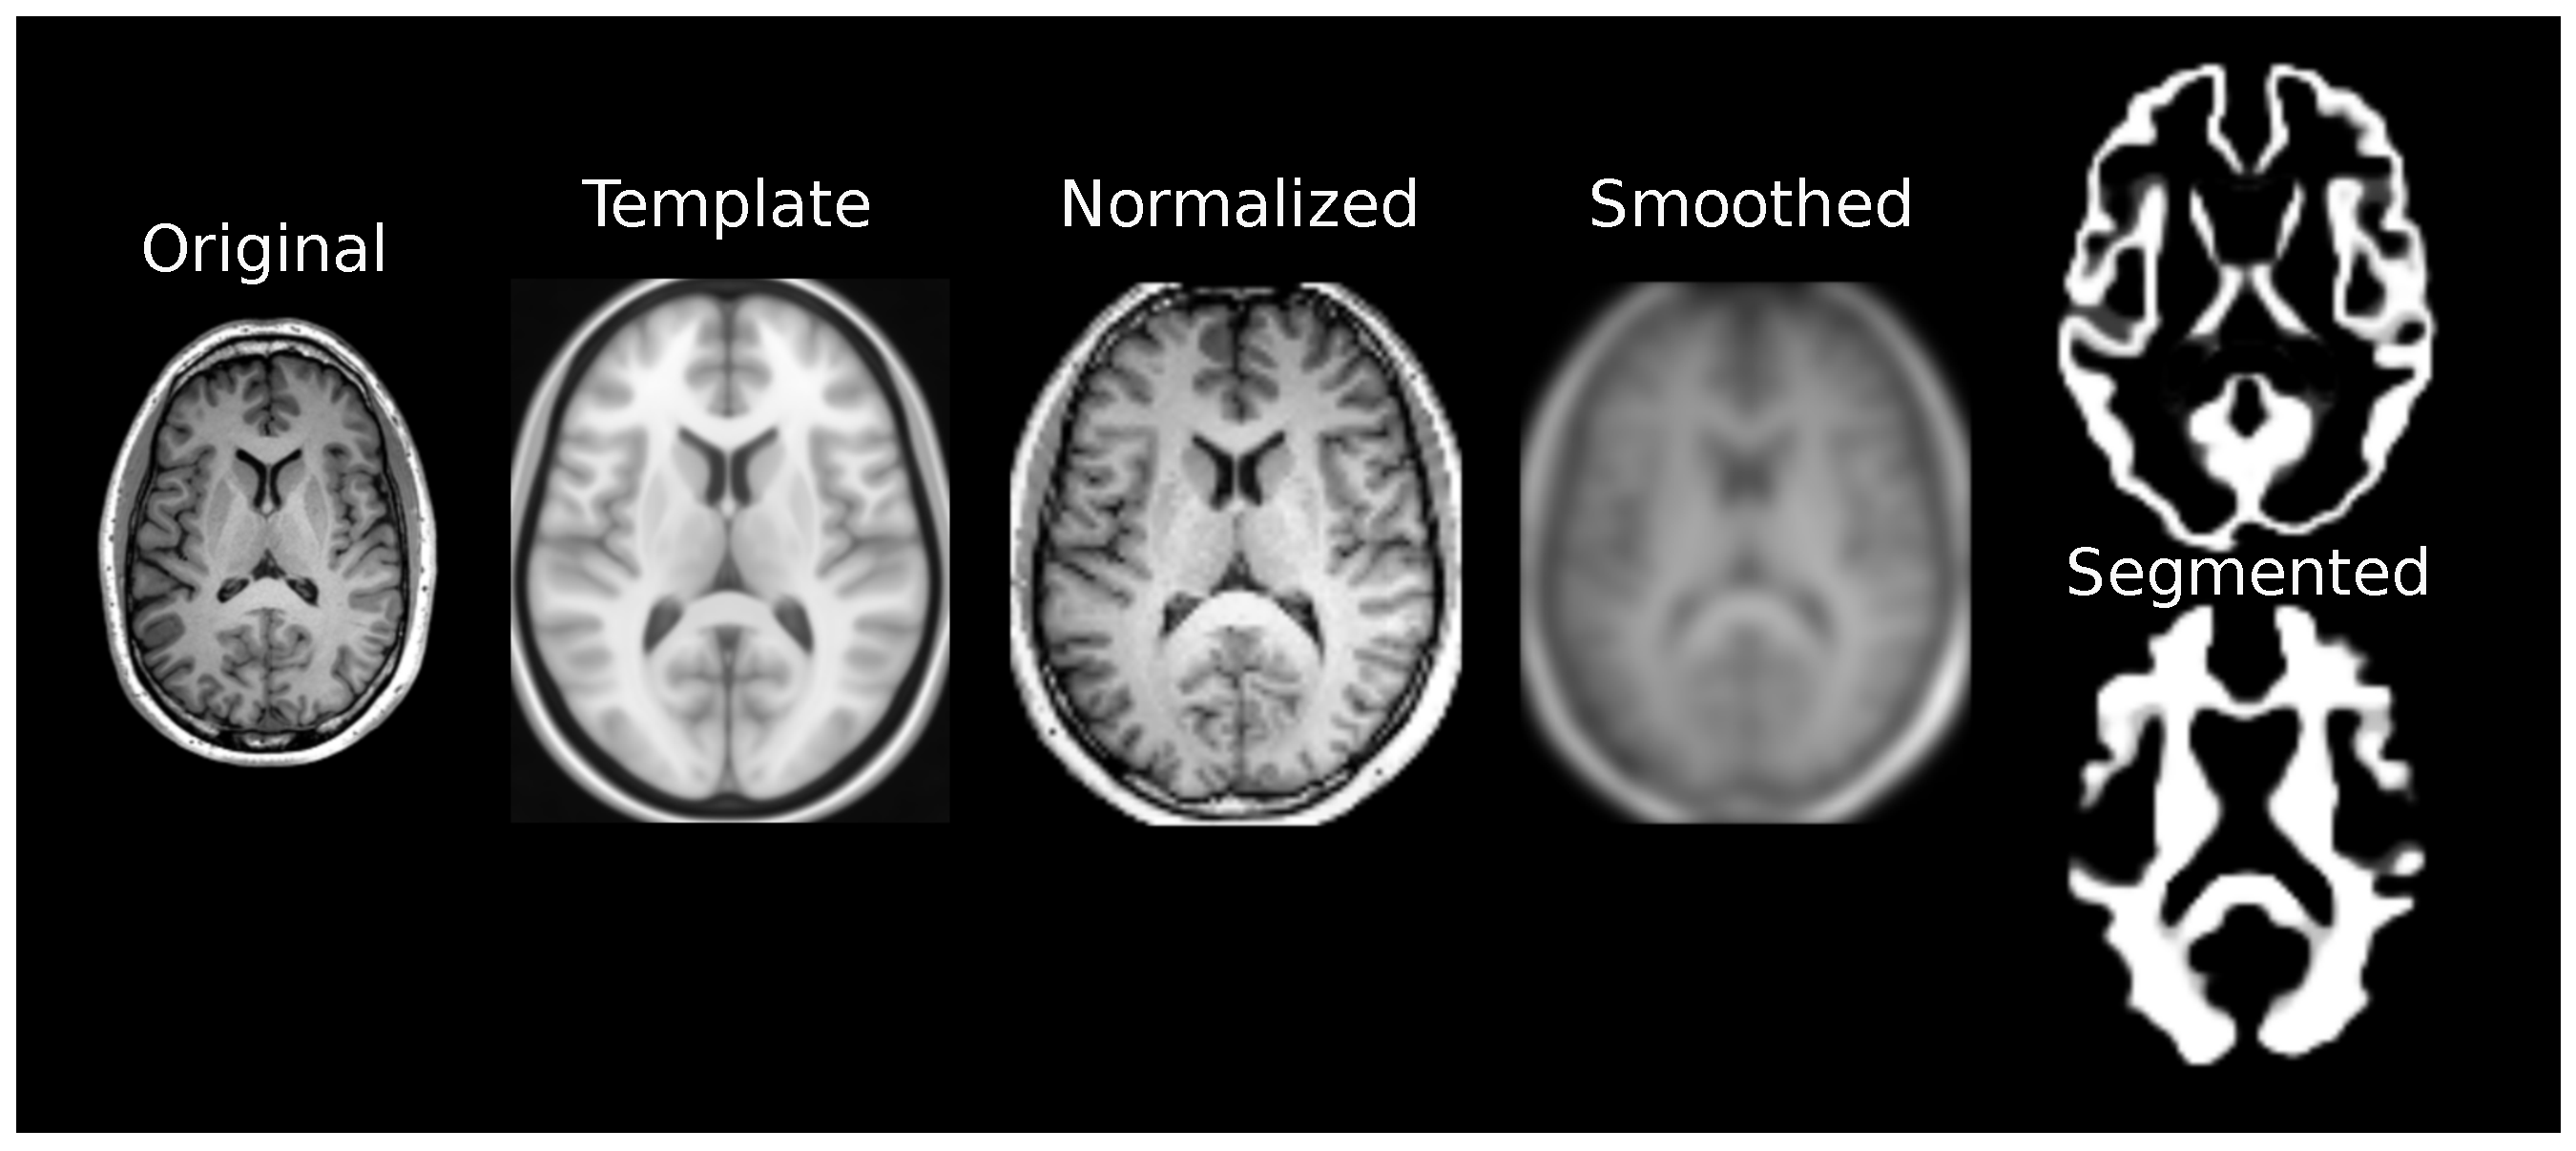
\includegraphics[width=.75\linewidth]{gfx/ch3/preProcessPL}
	\caption[Typical pre-processing pipeline in MRI]{Typical pre-processing pipeline in \ac{MRI}.}\label{fig:examplePreMRI}
\end{figure}

In this thesis, all the experiments in all image modalities involve spatial normalization. Smoothing, as well as segmentation, is only applied in some experiments that use \ac{MRI} images, such as the segmented images in Chapter~\ref{ch:sbm} or the whole-brain analysis performed in Chapter~\ref{ch:swpca}. 

\subsection{Spatial Normalization or Registration}
Spatial Normalization, also known as Registration, is the procedure that by which every subject's brain is mapped from their individual space to a standard reference system. Registered images allows our system to overcome the individual differences in position and anatomy by establishing a common reference space in which a given coordinate represent the same anatomical position in all brains in the dataset. 

There exist a number of pieces of software widely used for registering images, such as FreeSurfer \cite{Reuter2010} or FSL (in the FLIRT and FNIRT package) \cite{Smith2004}, most of them perform linear, non-rigid and elastic transformations or a combination of these. In this work we have used the software SPM8 \cite{spm_book} to perform registration of all the datasets, including \ac{MRI}, \ac{SPECT} and \ac{PET} images. So, from this moment, we will focus on the registration as performed in the \ac{SPM8}. 

Linear registration usually refers to the affine transformation, a matrix multiplication that includes 12 parameters for translation, rotation, scale, squeeze, shear and others: 
\begin{equation}\label{eq:affine}
	\left[\begin{matrix}
	x'\\y'\\z'\\1
	\end{matrix}\right]
	 = \left[\begin{matrix}
	 a_{00} & a_{01} & a_{02} & a_{03}\\
	 a_{10} & a_{11} & a_{12} & a_{13}\\
	 a_{20} & a_{21} & a_{22} & a_{23}\\
	 0 & 0 & 0 & 1\\
	 \end{matrix}\right]
	 \left[\begin{matrix}
	 x\\y\\z\\1
	 \end{matrix}\right]
\end{equation}

This matrix multiplication is performed globally, as it transforms the whole image, not accounting for local geometric differences. In equations \ref{eq:affine1}, \ref{eq:affine2} and \ref{eq:affine3} we give an example of the parameters that are computed for scale, translation and shear in 3D:

\begin{align}
\label{eq:affine1}
	\text{scale} &= 
	\left[\begin{matrix}
		 s_x  &0 & 0 & 0\\
		0 &s_y &0 &0\\
		0 &0 &s_z &0\\
		0 &0 &0 &1		
	\end{matrix}
	\right]\\
	\label{eq:affine2}
	\text{translation} &= 
	\left[
	\begin{matrix}
	1  &0 & 0 & \Delta x\\
	0 &1 &0 &\Delta y\\
	0 &0 &1 &\Delta z\\
	0 &0 &0 &1		
	\end{matrix}
	\right] \\
	\label{eq:affine3}
	\text{shear} &= 
	\left[\begin{matrix}
	1  &h_{xy}& h_{xz} & 0\\
	h_{yx} &1 &h_{yz} &0\\
	h_{zx} &h_{zy} &1 &0\\
	0 &0 &0 &1		
	\end{matrix}
	\right]
\end{align}

The combination of all these operations result in the estimation of the twelve parameters that we found in Eq.~\ref{eq:affine}, which are the ones used in \ac{SPM8}. The estimation of these parameters is performed via the optimization of a cost function, that in \ac{SPM8} can be the minimum squared difference between the source image and the template \cite{spm_book} in the case of within-modality registration, or the mutual information in between-modality registration. These functions are also used in FLIRT \cite{Jenkinson2001}, whereas FreeSurfer uses the Tukey's biweight function (in {\ttfamily mri\_robust\_template}) \cite{Reuter2012}.

After the affine transform, the software usually performs a fine-tuning step via nonrigid transformations, to account for relevant a\-na\-to\-mi\-cal differences between subjects. Nonrigid transformations range from the use of radial basis functions, physical continuum models and the large deformation models, or diffeomorphisms, that \ac{SPM8} uses. These procedures work by estimating a warp-field and then, apply it to the affine-registered images. An example of the differences of using only affine registration and applying diffeomorphisms can be found at Figure~\ref{fig:diffeomorphisms}.

\begin{figure}[bth]
	\myfloatalign
	\subfloat[Comparison in \ac{MRI}.]
	{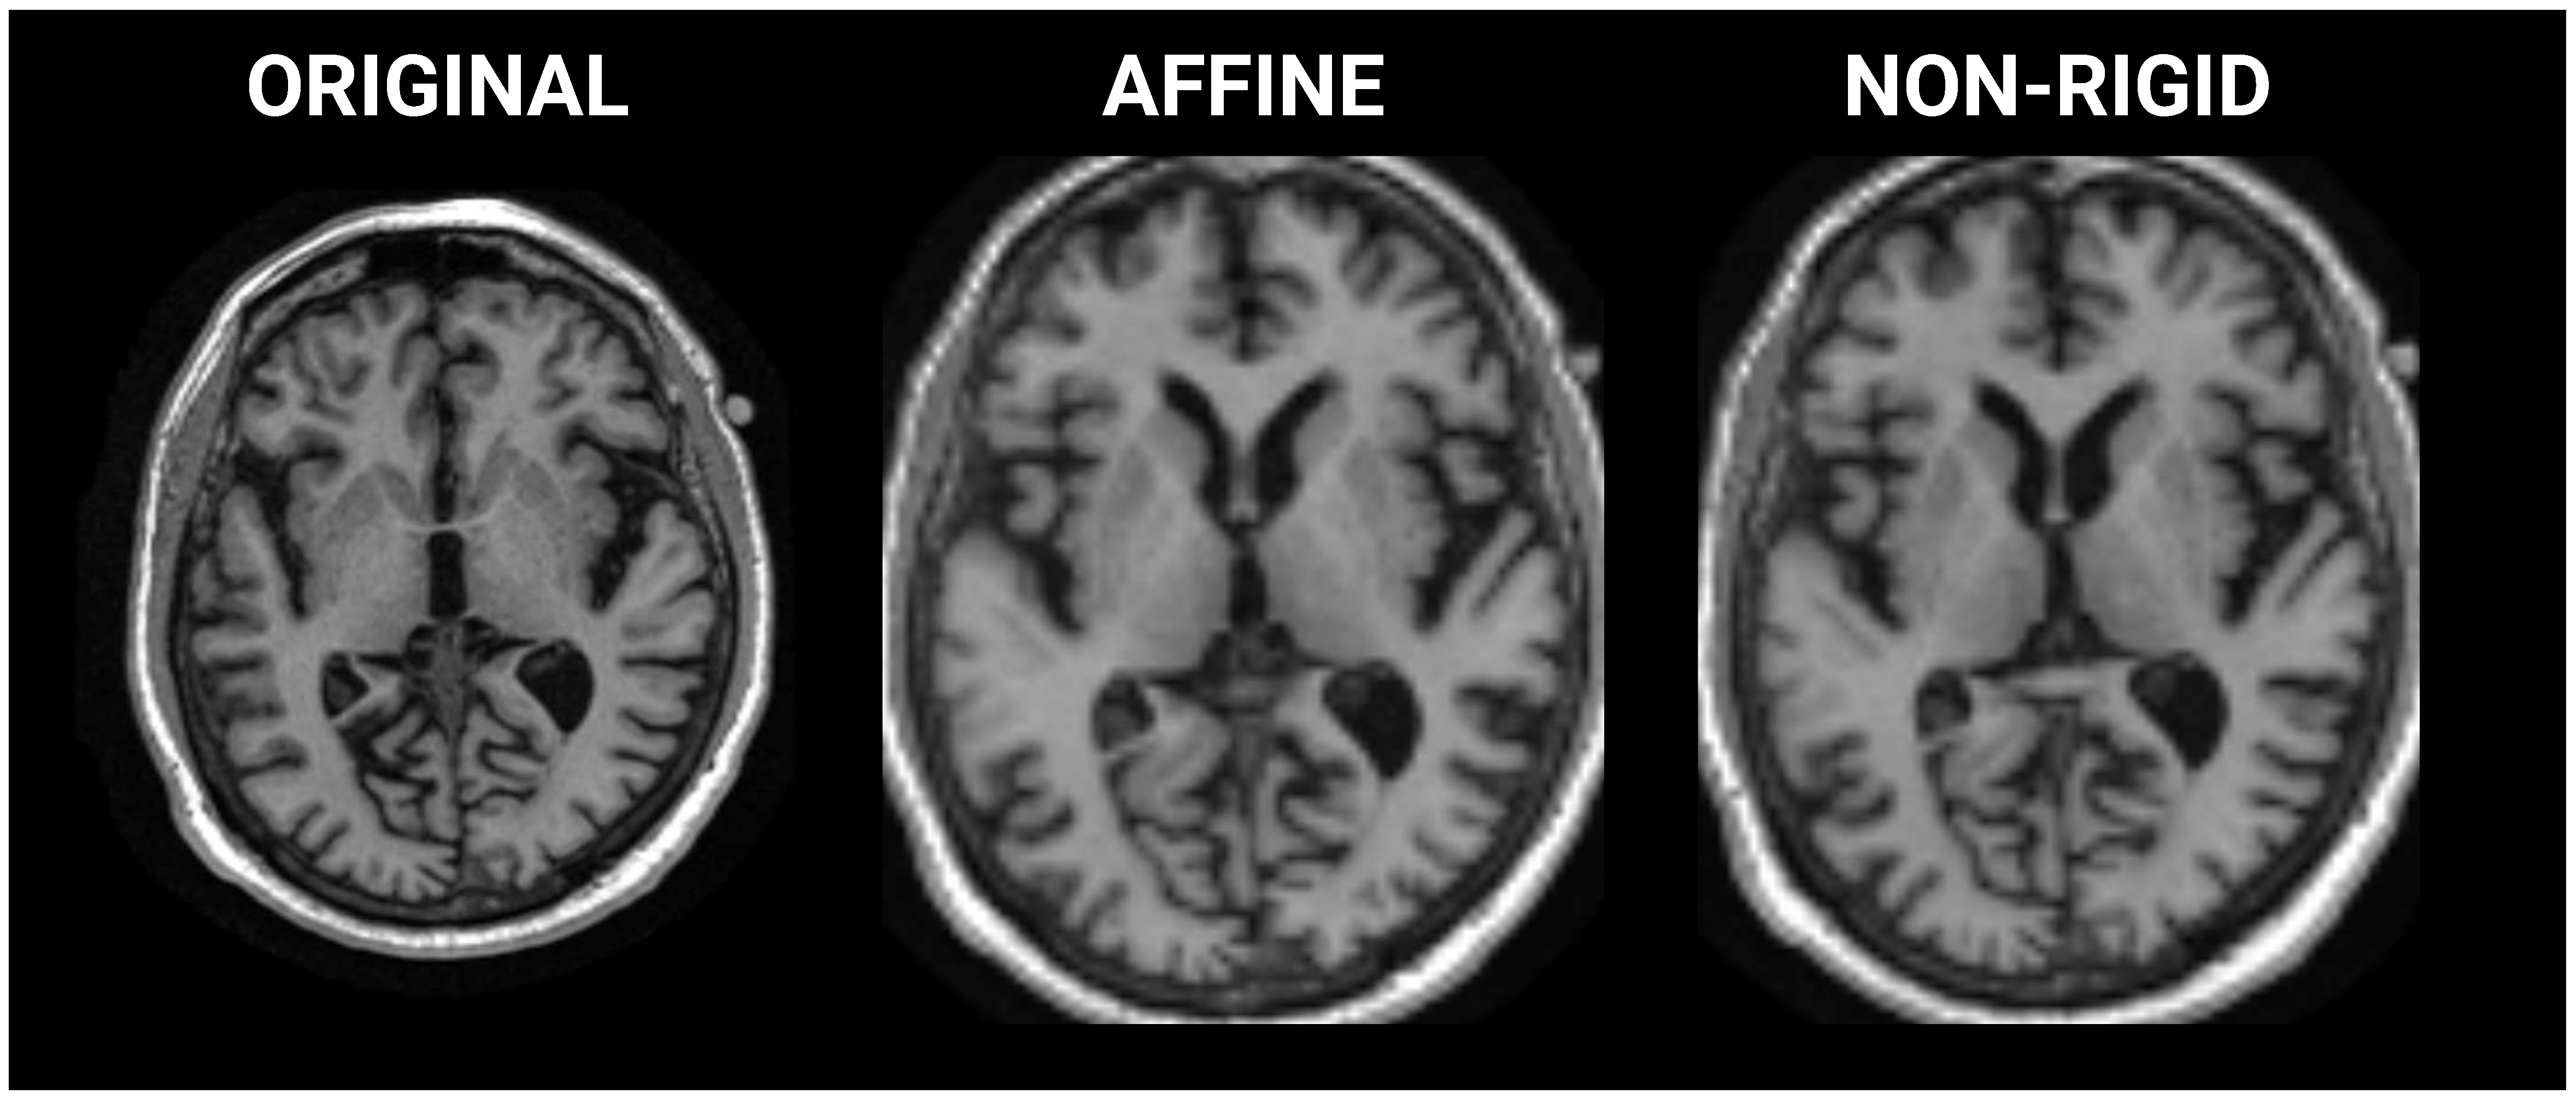
\includegraphics[width=.7\linewidth]{gfx/ch3/regComparisonMRI}}
	 \\
	\subfloat[Comparison in \ac{PET}.]
	{\includegraphics[width=.7\linewidth]{gfx/ch3/regComparisonPET}}
	\caption[Comparison of the affine registration and the application of non-linear transformations to the images]{Comparison of the affine registration and the application of non-linear transformations to both \ac{MRI} and \ac{PET} images of the same \ac{ADNI} subject.}\label{fig:diffeomorphisms}
\end{figure}


\subsubsection{Co-registration}
Sometimes we have several image modalities of the same subject, for example \ac{MRI} and \ac{PET} or functional \ac{MRI}, often acquired at the same time. In this particular case, we can use the higher resolution \ac{MRI} image to calculate the affine parameters and warping, and apply those to all modalities of the same subject. To do so, we perform a first co-registration, that is, a registration of the lower-resolution images (e.g. \ac{PET}) to its correspondent \ac{MRI} image. Being anatomically similar, the co-registration usually comprises a single affine transformation. Afterwards, we can proceed with the registration of that \ac{MRI} image to the template, and apply the same transformation to all its co-registered images. 

\subsubsection{The MNI Space}
In this thesis, all images are coregistered to the \acf{MNI} space \cite{Mazziotta2001}. This is the most widely used coordinate system, recently adopted by the International Consortium for Brain Mapping (ICBM) as its standard template. The three-dimensional coordinate system defined in \ac{MNI} was intended to replace the Tailarach space, a system based on a dissected brain, that was used to compose an atlas by Tailarach and Tournoux \cite{Talairach1988c}. The current template is known as ICBM152, and features the average of 152 normal \ac{MRI} scans matched to an older \ac{MNI} template using a nine parameter affine registration. 

\subsection{Segmentation}
When using \ac{MRI} images in this thesis, we often refer to \acf{GM} and \acf{WM} maps, which is the result of the segmentation of the original data. Segmentation aims at producing maps of the distribution of different tissues, and it generally addresses \ac{GM}, \ac{WM} and \ac{CSF} classes, although lately some software can output data for bone, soft tissue or very detailed functional regions and subregions \cite{Fischl2002}. 

In this thesis we have used the \ac{VBM} toolbox of the \ac{SPM8} software, which yields \ac{GM}, \ac{WM} and \ac{CSF} maps. It features an \ac{EM} algorithm to model the distribution of the tissue classes as a mixture of gaussians and, by combining this distribution-based information with tissue probability maps using a bayesian rule, the software produces joint posterior probability maps for each tissue. To clean up the segmentation maps, a series of iterative dilations and erosions are used. Finally, since brain regions are expanded or contracted at the spatial normalization step, we can scale the segmented maps using modulation, producing final maps where the total amount of grey matter is preserved. 

\section{Intensity Normalization}
Generally, structural modalities such as T1 and T2-weighted images are considered unitless, in contrast to functional imaging, in which each voxel's intensity represent the distribution of some biomarker, such as glucose metabolism, dopamine transporters, etc. These amounts are affected by many sources of variability that can affect the final values: contrast uptake, radiotracer decay time, metabolism, etc. Therefore, along with the previous spatial normalization, there is a need to normalize the intensities of the images, so that the amount they represent are comparable. 

In the case of intensity normalization, the method acts as a linear transformation of the image, preserving fundamental information such as contrast between regions. This approximation estimates the new intensity values $I'$ as: 
\begin{equation}
	I' = I/I_p 
\end{equation}
where $I_p$ is a constant parameter that is unique for each image. After this division, the new intensities would be directly comparable. The technique used to compute the normalization parameter varies, ranging from the simplest normalization to the maximum \cite{Salas-Gonzalez2009,Martinez-Murcia20129676} to complex methodologies that use assumptions about the image's \ac{PDF}. 

The \emph{normalization to the maximum} strategy computes $I_p$ as the average value of the 95th bin of the histogram of the image. In other words, this mean averaging the 5\% higher intensity values and use this mean as $I_p$. Another useful approach is the so-called \emph{integral normalization}, which computes $I_p$ as the sum of all values in the image. 

Other approaches involves some a-priori knowledge about the intensity distribution of normal subjects in a certain modality. This is the case of setting $I_p$ to the Binding Potential (BP), a ratio between the intensities at specific and non-specific areas \cite{Scherfler2005}. 

Finally, more advanced approaches use a general linear transformation of the image: 
\begin{equation}
	I' = a I + b
\end{equation}
The parameters $a$ and $b$ are so that the \ac{PDF} of a given matches a reference \ac{PDF}. There exist methods that use the histogram \cite{Arndt1996}, the gaussian distribution or the alpha-stable distribution \cite{Salas-Gonzalez2013}. In this latter case, the parameters $a$ y $b$ are computed as linear transformations of some distribution's parameters: 
\begin{equation}
	a = \frac{\gamma*}{\gamma}, \quad b = \mu* + \frac{\gamma*}{\gamma} \mu
\end{equation}
where $\gamma*$ and $\gamma$ are the dispersion parameters of the alpha-stable intensity distribution of the non-normalized and the reference image respectively, and $\mu*$ and $\mu$ are the location parameters of the same images. 

Despite traditionally structural modalities such as \ac{MRI} did not use intensity normalization, there exist a new tendency towards the use of \ac{qT1} and \ac{qT2} images \cite{Weiskopf2013} that provide biomarkers for absolute measures such as myelination, water and iron levels. This strategy is especially designed to overcome different sources of variability that affect multicentre studies, e.g. magnetic field inhomogeneity, noise, evolution of the scanners, etc. The role of those in multi-centre studies is addressed at Chapter~\ref{ch:swpca}. 

See Figure~\ref{fig:comparisonIntNorm} for a comparison between different strategies of intensity normalization on the same images. 

\begin{figure}[bth]
	\myfloatalign
	\subfloat[Normalization to the Maximum.]
	{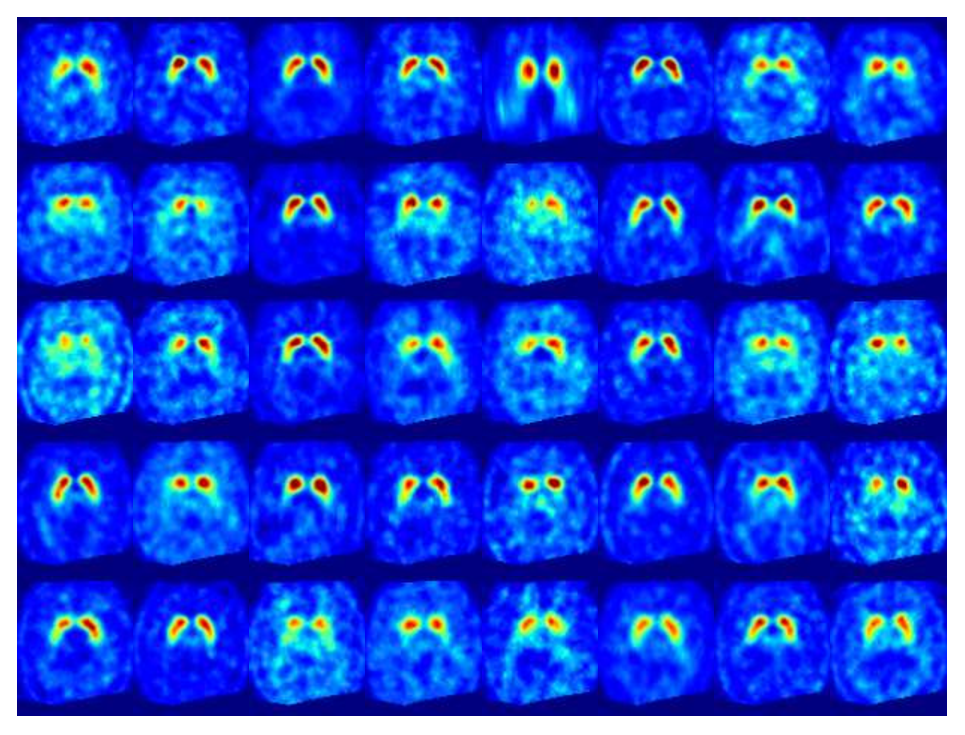
\includegraphics[width=.45\linewidth]{gfx/ch3/norm_max.eps}}\quad
	\subfloat[Integral Normalization.]
	{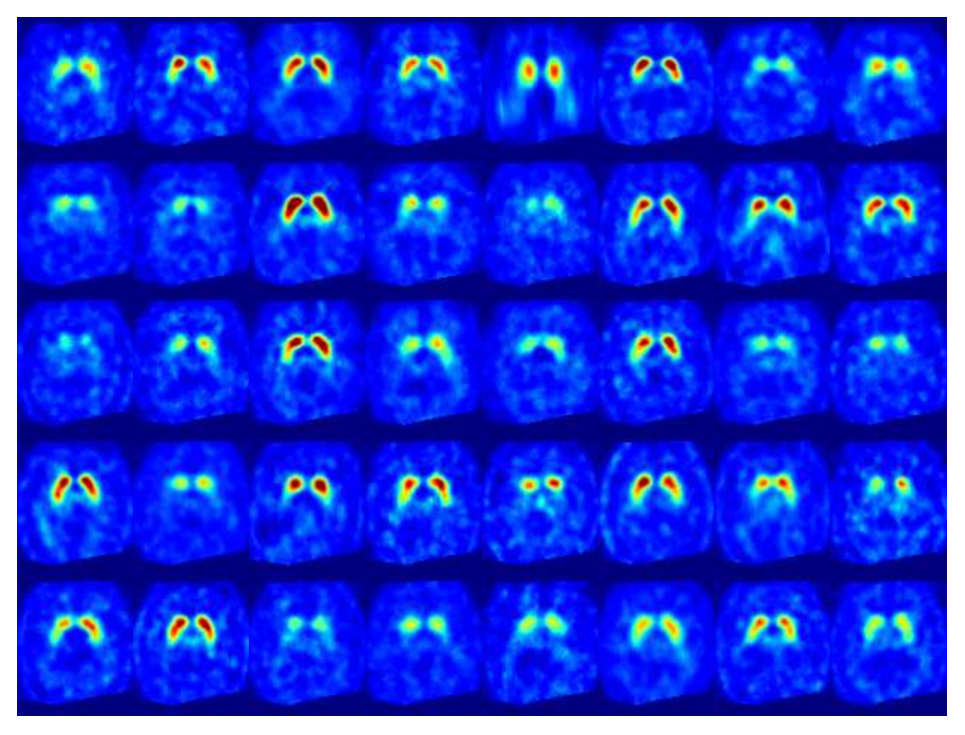
\includegraphics[width=.45\linewidth]{gfx/ch3/norm_int.eps}}\\
	\subfloat[Normalization using $\alpha$-stable distribution.]
	{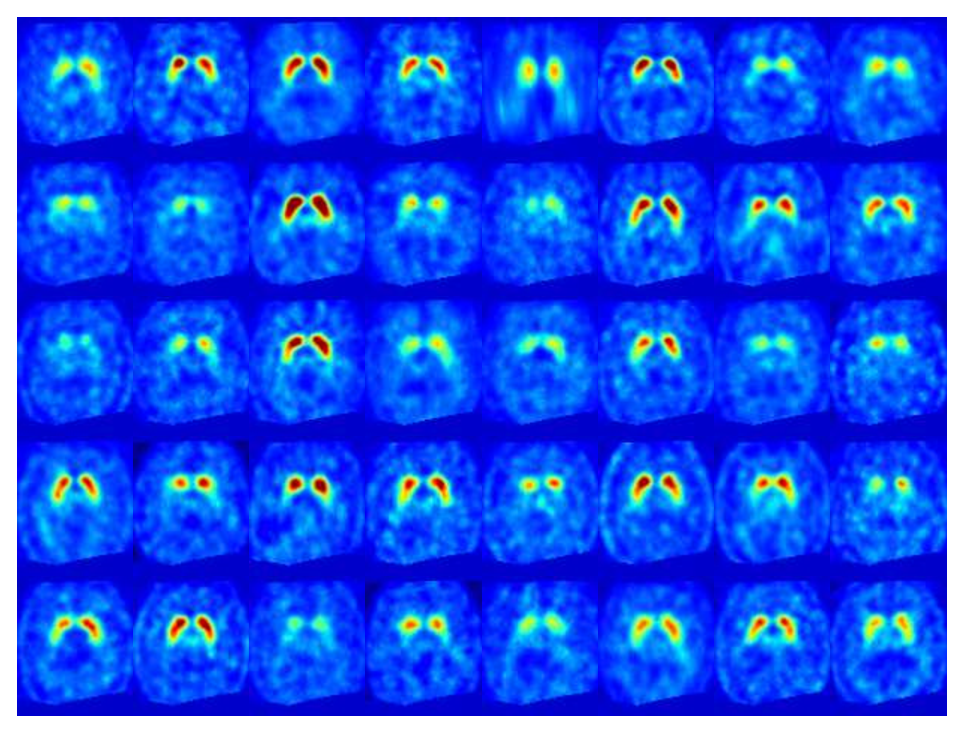
\includegraphics[width=.45\linewidth]{gfx/ch3/norm_est.eps}}
	\caption{Comparison between different types of intensity normalization, applied to the VDLN-DAT dataset (see Appendix~\ref{ch:datasets}).}\label{fig:comparisonIntNorm}
\end{figure}
%DONE


\section{Evaluation Parameters and Methodology}\label{sec:validation}
\subsection{Cross-validation}

The classification was validated using stratified 10-fold
cross-validation (Kohavi, 1995). In brief, 9 subsets of the dataset
were used for extraction of the PCs and training of the classifier with
the remaining subset used for testing. This procedure was repeated for
each subset, repeated 10 times to avoid possible bias and random
effects of the partitions. The average and standard deviation of the
accuracy (acc), sensitivity (sens) and specificity (spec) values for
each repetition were recorded. 

\subsection{Classification Performance}

The proposed methodology has been tested on the three previously described databases, using a cross-validation method called leave-one-out to extract several performance parameters: accuracy, sensitivity, specificity, positive likelihood (PL) and negative likelihood (NL). This method achieves an almost unbiased error estimate, however it might be affected by the database topology, reason why we used different databases to test our method.

Along with the widely used sensitivity, specificity and accuracy (which are prevalence dependent), we use the Positive and Negative Likelihood ratios (PL and NL) to provide some prevalence independent parameters that are also widely used in clinical medicine, where values of PL greater than 5 or NL values less than 0.2 can be applied to the pre-test probability of a patient having the disease tested for to estimate a post-test probability of the disease state existing \cite{McGee2002}. A positive result for a test with an PL of 8 adds approximately 40\% to the pre-test probability that a patient has a specific diagnosis. 

To provide a better understanding of the accuracy distribution (mean, range, skewness), we have made use of the box plot (Fig. \ref{fig:features_acc_distances}). In these plots, the median for each group of data is indicated by the red center line, and the first and third quartiles are the edges of the blue box, which is known as the inter-quartile range (IQR). The extreme values (within 1.5 times the inter-quartile range from the upper or lower quartile) are the ends of the lines extending from the IQR. Points at a greater distance from the median than 1.5 times the IQR are plotted individually, representing potential outliers. 



%************************************************
\chapter{Image Decomposition}\label{ch:decomposition}
%************************************************

In this chapter, we will focus on those \ac{CAD} systems that use a combination of an image decomposition method and feature selection by means of hypothesis testing. These variety of methods have been published in \cite{Martinez201141,Martinez-Murcia20129676,Martinez-Murcia2013255,Martinez-Murcia201458}. 

Image decomposition methods model a set of samples as a linear combination of $c$ latent variables, also known as components. These variables can be considered as the basis of a $c$-dimensional space where each sample is represented by a feature vector of length $c$. The $i$-th neuroimage in our dataset can be therefore decomposed as: 

\begin{equation}\label{eq:generalDecomposition}
	\mathbf{x}_i = s_0 \mathbf{w}_0 + s_1 \mathbf{w}_1 + \dots + s_c \mathbf{w}_c + \boldmath\epsilon = \mathbf{s}\mathbf{W} + \boldmath\epsilon
\end{equation}

Where $s_i$ is the coordinate (or component score) of the current image in the $i$-th dimension of the new space defined by all the base vectors $\mathbf{w}_i$ (component loadings), and $\boldmath\epsilon$ is the error of the estimation. Figure \ref{fig:decomposition_overview} shows an illustration of the process. 

\begin{figure}[tph]
	\centering
	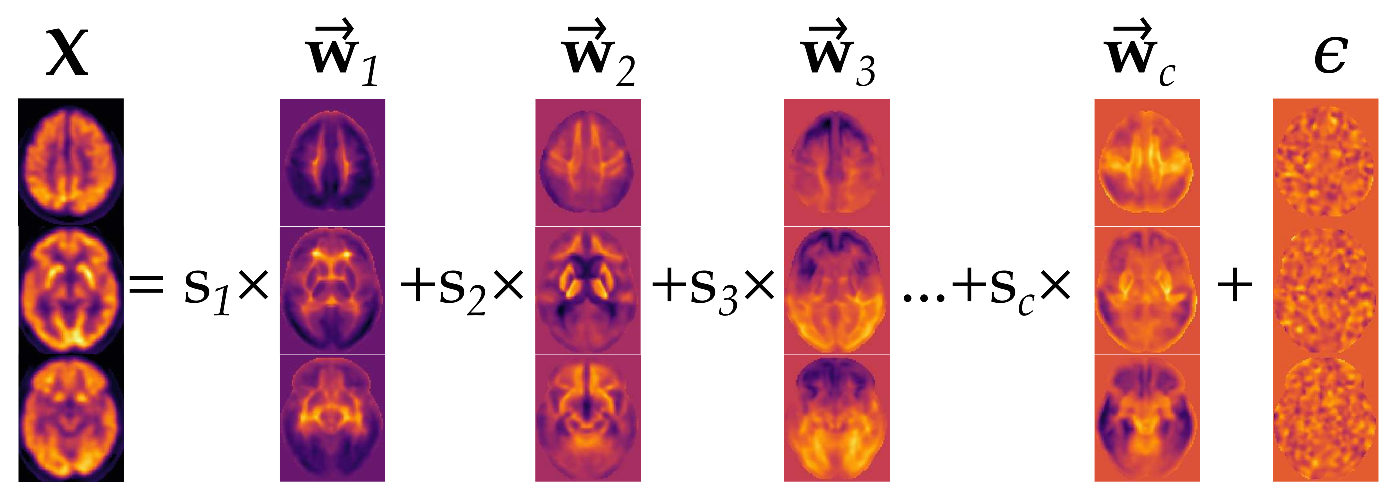
\includegraphics[width=0.9\linewidth]{Graphics/ch4/decomposition_overview}
	\caption[Illustration of how decomposition algorithms work.]{Illustration of how decomposition algorithms such as \ac{FA} and \ac{ICA} work on a \ac{PET}-FDG brain image.}
	\label{fig:decomposition_overview}
\end{figure}

Many signal decomposition techniques are used in the literature, for example \ac{PCA} or \ac{PLS} \cite{Spetsieris2009,Illan2011,Towey2011,Segovia2013,Khedher2015}. We will focus on two less known decomposition algorithms \acf{FA} and \acf{ICA}, which we will integrate in different \ac{CAD} systems using a pipeline similar to the one displayed at Figure~\ref{fig:pipelineDecomposition}. This pipeline involves feature selection (for reducing the dimensionality), decomposition of the feature vectors and classification.
 
\begin{figure}[tph]
	\centering
	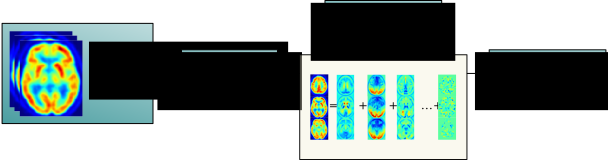
\includegraphics[width=0.7\linewidth]{Graphics/ch4/01-flowdiagram}
	\caption[Illustration of the system used in Chapter~\protect\ref{ch:decomposition} .]{Illustration of the system used in Chapter~\protect\ref{ch:decomposition}.}
	\label{fig:pipelineDecomposition}
\end{figure}

\section{Feature Selection}
Feature selection is the first strategy used for feature reduction \cite{Martinez-Murcia2016b}, and it is often used along with feature extraction in order to build more complex pattern recognition systems. It refers to any strategy intended to find a subset of the original features containing the more suitable ones according to a certain criterion. Therefore, irrelevant features are discarded, and resultant models are faster and more cost-effective \cite{Guyon03}. However, it usually requires an additional optimization to find the parameters for the optimal feature subset, and furthermore, it is impossible to guarantee that the optimal features for the subset are the same of the full feature set \cite{DaelemansHosteMeulderEtAl2003}. 

In this work, we will use filtering methods to perform feature selection. As we introduced in Section~\ref{sec:mvanalyses}, filtering methods are based on the computation of a feature relevance score directly on the data. The relevance score is used to sort the different features, discarding those with a lower score, and it is usually computed independently for each feature, in what is called a univariate approach \cite{SaeysInzaLarranaga2007}. 

Feature selection can be used before or after feature extraction. When using computationally-intensive algorithms such as \ac{FA} or especially \ac{ICA}, the selection of best features prior to the decomposition is key to obtain high performance while keeping the computation times small \cite{Martinez201141,Martinez-Murcia20129676}. This also removes noise in some cases where the decomposition algorithm cannot compute correctly the variance. 

\begin{figure}[bth]
	\myfloatalign
	\subfloat[$t$-test.]
	{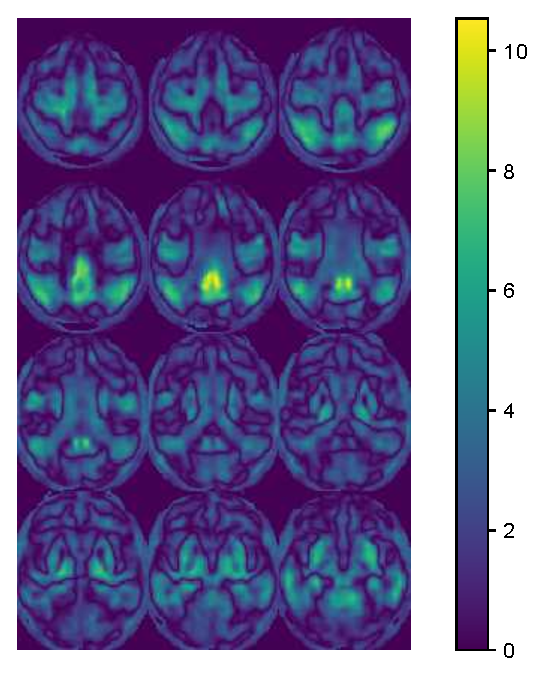
\includegraphics[width=.3\linewidth]{Graphics/ch4/ttest_map.eps}\label{fig:ttest_map}}\quad
	\subfloat[\ac{KL} divergence.]
	{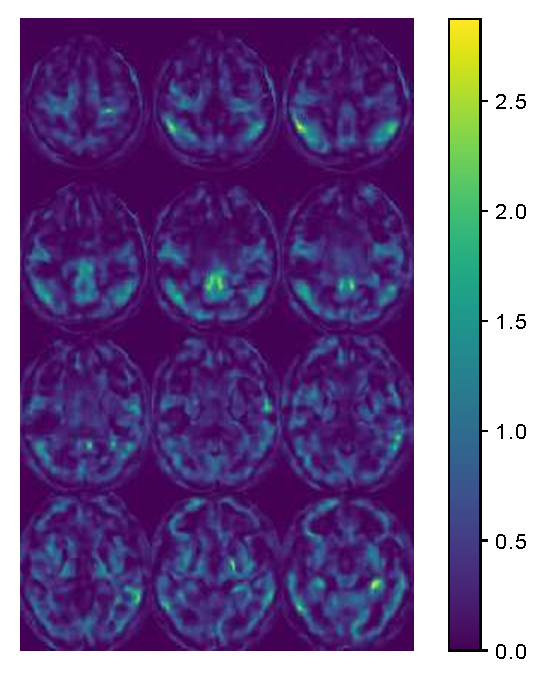
\includegraphics[width=.3\linewidth]{Graphics/ch4/kl_map.eps}\label{fig:kl_map}}\quad
	\subfloat[\ac{MWW} $U$-test.]
	{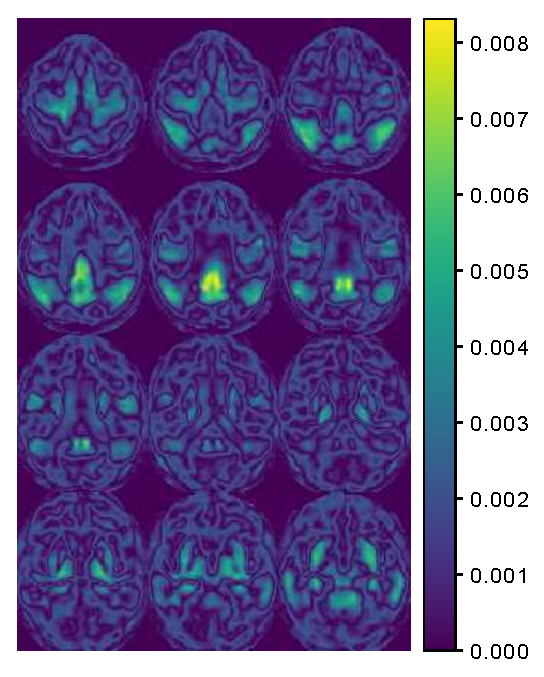
\includegraphics[width=.3\linewidth]{Graphics/ch4/wilcoxon_map.eps}\label{fig:wilcoxon_map}}
	\caption[Comparison between the different filtering methods.]{Comparison between the different filtering methods, and the regions selected by them, in the ADNI-PET dataset. }\label{fig:comparisonSelection}
\end{figure}

Three feature selection algorithms have been used in this thesis, not only in the \ac{CAD} systems proposed in this chapter, but in many other models that will be presented later: the $t$-Test, the Kullback-Leibler divergence or Relative Entropy, and the Mann-Whitney-Wilcoxon rank test. 

\subsection{$t$-test}
The $t$-test is an old friend of statisticians. In this work we will use the independent two-sample $t$-test \cite{Fay10}. It quantifies the differences between two classes using an assumption of independent variances. Let $X_i^f$ a vector containing the $f$-th feature of all elements in class $i$. The $t$-score of the $f$-th feature can be computed as:

\begin{equation}
t_f = \frac{\bar{X}_1^f - \bar{X}_2^f}{\sqrt{\frac{\sigma_{X_2^f}^2+\sigma_{X_1^f}^2}{n}}}
\end{equation}
where $\sigma_{X_i^f}^2$ is the variance and $\bar{X}_i^f$ is the average of the $f$-the feature within class $i$. The $t$-test is extensively used in the neuroimaging community, and it is the basis for the \ac{SPM} and \ac{VBM} analyses \cite{spm_book}. See figure~\ref{fig:ttest_map} for an example of the $t$-test computed on the ADNI-PET database.

\subsection{Kullback-Leibler Divergence} 
Another alternative is the \acf{KL} divergence, also known as Relative Entropy. It is a non-symmetric measure of the difference between two probabilities distributions. Let us assume that $X_1^f$ and $X_2^f$, the vectors containing the $f$-th feature of all elements in class $i$, are two discrete random variables. Therefore, the \ac{KL} divergence can be calculated with equation \ref{kullback} \cite{Theodoridis1999}.

\begin{equation}\label{kullback}
KL_f = \left(\frac{\sigma_{X_2^f}^2}{\sigma_{X_1^f}^2} +\frac{\sigma_{X_1^f}^2}{\sigma_{X_2^f}^2} -2 \right) + \frac{1}{2}\left(\bar{X}_2^f-\bar{X}_1^f\right)^2\left(\frac{1}{\sigma_{X_1^f}^2} + \frac{1}{\sigma_{X_2^f}^2}\right)
\end{equation}
using the same notation than in $t$-test. See figure~\ref{fig:kl_map} for an example of the computed \ac{KL} divergence on the ADNI-PET database.

\subsection{Mann-Whitney-Wilcoxon} 
The \acf{MWW} rank test, also known as $U$-test, assigns a rank to all values in the vector corresponding to the $f$-th feature, $X^f$, without considering any class. The method used to assign a rank is the `average', which means that each value is assigned with the average of the ranks that would have been assigned to all the tied values. This means that, for example, in the case of the vector $X^f=(0,2,3,2)$, the ranks assigned to each element would be $R^f=(1,2.5,4,2.5)$. 

Let $n_1$ and $n_2$ be the number of elements in class 1 and 2 respectively, and $R^f$ the vector of ranked elements. We proceed by selecting the first $n_1$ elements in $R^f$ by: 
\begin{equation}
	R^f_{n_1} = {R^f_i} \quad \forall i\in(0,n_1)
\end{equation}

The $U$-score for the $f$-th feature and the first class will be: 
\begin{equation}
	U_1^f = n_1 n_2 + n_1 \frac{n1+1}{2} - \sum R^f_{n_1}
\end{equation}

And the it can be computed for the second class as the remainder: 
\begin{equation}
	U_2^f = n_1 n_2 - U_1
\end{equation}

The final $U^f$ can be assigned to either $U_1^f$, $U_2^f$ or $\min{U_1^f,U_2^f}$ \cite{Fay10}, but the usual approach nowadays is to assign $U^f=U_2^f$. Unlike $t$-test, \ac{MWW} test does not assume any prior distribution, and therefore is less likely than it to spuriously indicate significance because of the presence of outliers. Under the normal distribution, it performs relatively similar \cite{Fay10}. See figure~\ref{fig:wilcoxon_map} for an example of the \ac{MWW} $U$-test computed on the ADNI-PET database.

\section{Decomposition Algorithms}
The feature selection algorithms presented above will perform a significant feature reduction, from hundreds of thousands of voxels to a few thousands. These few thousands voxels are considered the best in discriminating between \ac{CTL} and affected subjects in each of the diseases. The feature selection strategy can be thought of as a mask, in which only the most relevant regions according to the tests are selected (see Figure~\ref{fig:comparisonSelection}). 

However, this number of features is still large, and therefore, further feature reduction can be applied by performing a decomposition of the masked regions. We have used two algorithms in our \ac{CAD} systems: \acf{FA} and \acf{ICA}.

\begin{figure}[bth]
	\myfloatalign
	\subfloat[Original]
	{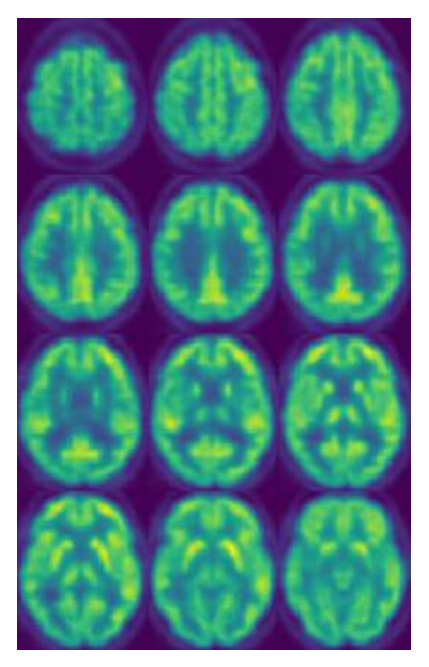
\includegraphics[width=.3\linewidth]{Graphics/ch4/originalImage.eps}}\quad
	\subfloat[\ac{FA} reconstruction]
	{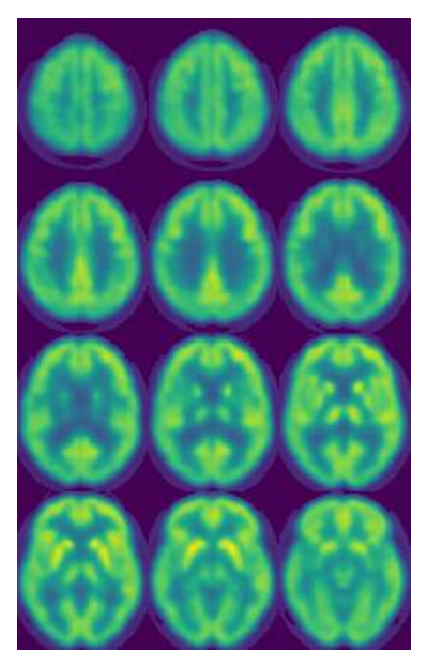
\includegraphics[width=.3\linewidth]{Graphics/ch4/transformedFA.eps}}\quad
	\subfloat[\ac{ICA} reconstruction]
	{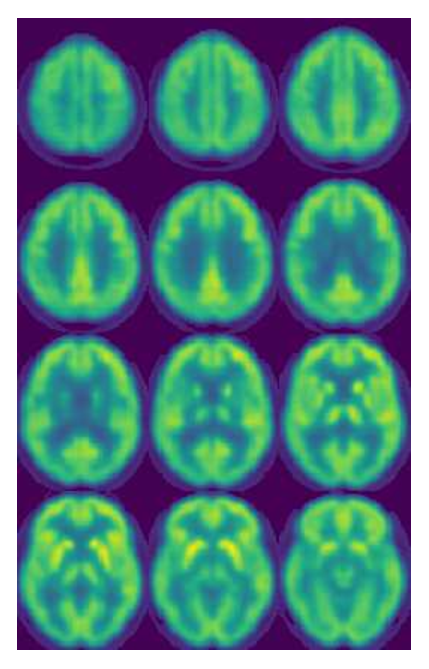
\includegraphics[width=.3\linewidth]{Graphics/ch4/transformedICA.eps}}
	\caption[Original PET image and its reconstruction using FA or ICA.]{Original PET image from the ADNI-PET dataset, and examples of reconstruction using \ac{FA} or \ac{ICA}, with 10 components.}\label{fig:comparisonReconstructions}
\end{figure}


\subsection{Factor Analysis}
\acf{FA} was used in \cite{Martinez201141,Martinez-Murcia20129676} to perform feature extraction in \ac{CAD} systems. This strategy assumes that each image in the database is a realization of a given experiment. \ac{FA} then models each of the $N$ observations (or subjects) as the expression of $c$ unobserved variables, known as factors. The model follows the general decomposition equation (Eq. \ref{eq:generalDecomposition}), but assuming that the dataset matrix $\mathbf{X}$ is zero-centred. That is, that we have subtracted the mean prior to the computation. In matrix form, Eq. \ref{eq:generalDecomposition} can be rewritten as:

\begin{equation}\label{eq:factoranalysis}
\mathbf{X} -\boldsymbol{\mu}= \mathbf{S}\mathbf{W} +  \boldsymbol{\epsilon}
\end{equation}

The columns of $\mathbf{W}$ are known as factors, and the rows of $\mathbf{S}$ are known as loadings  (similar to the concept of component loading and component scores in \ac{PCA}). Thanks to this, we can convert the original dataset $\mathbf{X}$ of size $N\times f$ into $\mathbf{S}$, of size $N\times c$. The procedure of computing the decomposition imposes some assumptions on $\mathbf{W}$: 
\begin{itemize}
	\item $\mathbf{W}$ and $\boldsymbol{\epsilon}$ must be independent. 
	\item $E[\mathbf{W}] = 0$. 
	\item $\text{Cov}(\mathbf{W}) = \mathbf{I}$, which ensures that the factors are uncorrelated. 
\end{itemize}

Now we can rewrite Eq.~\ref{eq:factoranalysis} as:
\begin{equation}\label{eq:fastep1}
	\text{Cov}(\mathbf{X} -\boldsymbol{\mu})= \text{Cov}(\mathbf{S}\mathbf{W} +  \boldsymbol{\epsilon})
\end{equation} 

Under the previous constraints, and setting $\boldsymbol{\Sigma} = \text{Cov}(\mathbf{X} -\boldsymbol{\mu})$, Eq.~\ref{eq:fastep1} becomes:
\begin{equation}
	\boldsymbol{\Sigma} = \mathbf{S}\text{Cov}(\mathbf{W})\mathbf{S}^T - \text{Cov}(\boldsymbol{\epsilon})
\end{equation}

Since $\text{Cov}(\mathbf{W}) = \mathbf{I}$, and making $\text{Cov}(\boldsymbol{\epsilon})=\boldsymbol{\Psi}$, the diagonal matrix containing the specific variances of the reconstruction error, we obtain the alternative form of \ac{FA}: 
\begin{equation}
\boldsymbol{\Sigma} = \mathbf{S}\mathbf{S}^T - \boldsymbol{\Psi}
\end{equation}

The mean $\boldsymbol{\mu}$, and the matrices $\mathbf{S}$ and $\boldsymbol{\Psi}$ are obtained via Maximum Likelihood estimation. To guarantee an unique solution, we impose that $\mathbf{S}^T\boldsymbol{\Psi}^{-1}\mathbf{S}$ is a diagonal matrix. Then, we obtain the parameters by maximizing the log-likelihood given by the following expression: 
\begin{equation}
	\ell(\mu,\mathbf{S},\boldsymbol{\Psi}) = - \frac{np}{2}\log{2\pi}- \frac{n}{2}\log{\left|\mathbf{SS}^T + \boldsymbol{\Psi}\right|} - \frac{1}{2}\sum_{i=1}^{n}(\mathbf{x}_i-\mu)^T(\mathbf{SS}^T+\boldsymbol{\Psi})(\mathbf{x}_i-\mu)
\end{equation} 

\ac{FA} differs from \ac{PCA} mainly because it performs an estimation of the noise, and needs the number of factors $c$ as an input. Choosing $c$ is not a naive task. A large $c$ can yield a small reconstruction error, but the factors will not be representative enough, leading to overfitting of the subsequent model. Conversely, a small $c$ can lead to a large reconstruction error, causing information loss. We have computed the reconstruction error variance over the ADNI-PET dataset, and plotted it in Figure~\ref{fig:error} (similar graphs can be obtained for other databases. This proves that the error is assymptotical as we increase $c$, and therefore, once arrived at certain error, the improvements are not significant. 

\begin{figure}[ht]
	\centering
	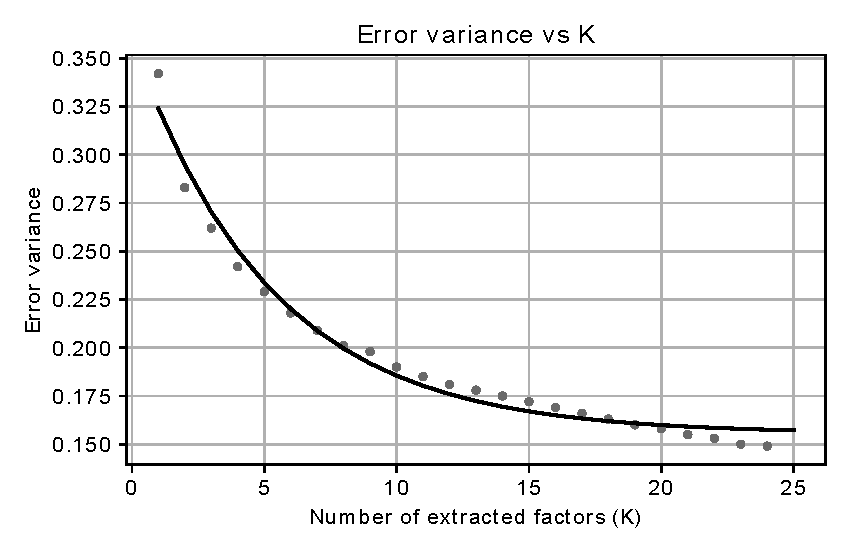
\includegraphics[width=0.5\linewidth]{Graphics/ch4/varError-K-ADNI}
	\caption{Specific variance of reconstruction error $\Psi$ using \ac{FA}, in function of number of factors extracted ($K$) for ADNI-PET database (the behaviour is similar in other datasets).}
	\label{fig:error}
\end{figure}


\subsection{Independent Component Analysis}
\cite{Martinez-Murcia2013255,Martinez-Murcia201458}

\acf{ICA} \cite{Hyvarinen2000}, is a statistical technique that represents a multidimensional random vector as a lineal combination of non-gaussian random variables (the so-called ''independent components'') to be as independent as possible, and has been used widely on segmentation and clustering of medical images \cite{DeMartino2007,Alvarez2009}. It can be considered as a non-gaussian version of Factor Analysis. Assume that we observe $n$ lineal mixtures $\mathbf{x}_1, \mathbf{x}_2, \ldots, \mathbf{x}_n$ of length $N$ that can be modelled as an expression of $K$ independent components (IC). These independent components are defined as $\mathbf{S} = (\mathbf{s}_1, \mathbf{s}_2, ... \mathbf{s}_K)$, where each $\mathbf{s}_K$ vector has a length of $N$. So, each random vector $\mathbf{x}_n$ can be described as a linear combination of $K$ independent components: 

\begin{equation}
\mathbf{x_n} = a_{1n}\mathbf{s}_1 + a_{2n}\mathbf{s}_2 + \ldots + a_{Kn}\mathbf{s}_K
\end{equation}

Without loss of generality we can assume that both the observed vectors and the independent components are are zero mean. If the previous conditions are not met, the $\mathbf{x}$ variables can be centered by subtracting the sample mean. To use a vector-matrix notation, more convenient in this case, we denote as matrix $\mathbf{X}$ the random vector whose elements are $\mathbf{x}_1, \ldots, \mathbf{x}_n$. We also denote as $\mathbf{A}$ the matrix that contains all $a_{Kn}$ elements, the ''mixing matrix'' that projects each image into the space defined by the IC. Using this notation, the mixing model above remains as follows: 

\begin{equation}\label{eq:ica}
\mathbf{X}=\mathbf{A}\mathbf{S}
\end{equation}

The starting point of ICA is the assumption that all components $\mathbf{s}_K$ are are statistically independent. To measure independence, we assume that all independent components have a non-gaussian statistical distribution. It is assumed that a sum of independent signal trends to gaussianity, so if non-gaussianity is maximized with any independence criteria $F$, for instance, the kurtosis or negentropy, we obtain signals that are more independent than the previous ones \cite{Hyvarinen1999,Hyvarinen2000}.
After estimating the matrix $\mathbf{A}$, we can compute its inverse, $\mathbf{W}$ and obtain the projection $\mathbf{S}$ of the images in the dataset into the IC space with: 
\begin{equation}
\mathbf{S} = \mathbf{W}\mathbf{X}
\end{equation}

\subsubsection{FastICA}
Adaptive algorithms based on gradient descend can be problematic when they are used on an environment in which adaptation is not necessary, like this case. The convergence is often slow, and depends on the choice of convergence parameters. As a solution to this problem, block algorithms based on fixed-point iteration \cite{Oja1997,FastICA99} can be used. In \cite{Oja1997} a fixed-point algorithm based on kurtosis is introduced. In \cite{FastICA99}, this algorithm, known as FastICA, is generalized to general contrast functions. The single unit FastICA algorithm has the following form:
\begin{equation}
\mathbf{w}(k) = E\lbrace\mathbf{x}g(\mathbf{w}(k-1)^T\mathbf{x})\rbrace -E\lbrace g'(\mathbf{w}(k-1)^T\mathbf{x})\rbrace\mathbf{w}(k-1)
\end{equation}
where the loadings vector $\mathbf{w}$ is normalized to unit norm in each iteration, and the function $g(x)$ is a derivative of the contrast function $G$ defined in \cite{Hyvarinen1999}. The expected values are estimated in practice by using the mean of a significantly high number of samples of the input data. 
The speed of convergence of the fixed-point algorithms is clearly superior to more neural algorithms. Improvements between 10 and 100 times the speed are observed frequently \cite{Giannakopoulos1998}. 


% AQUÍ EMPIEZA LO QUE HEMOS ESCRITO YA. 
\section{Results}
In this work we will analyse the behaviour of the system proposed in the introduction and illustrated at Figure~\ref{fig:pipelineDecomposition}. The system comprises the selection of the most relevant voxels using filtering methods (we will focus on $t$-test, relative entropy and wilcoxon) and a feature decomposition of these using either \ac{FA} or \ac{ICA}. Finally, the feature vectors are classified using a \ac{SVC} with linear kernel, and performance values are obtained via cross-validation (see Section~\ref{sec:validation} for more information). 

We vary the number of selected voxels and the number of factors or components depending on the algorithm and the dataset used and evaluate the system with those characteristics. That way, we obtain an estimation of the performance of the system in different situations, so that we can draw conclusions on the disease patterns and the ability of the system in the detection of different diseases. 

\subsection{Alzheimer's Disease}
We begin by applying the proposed feature selection plus decomposition pipeline to the two functional neuroimaging datasets: ADNI-PET and VDLN-HMPAO. For this experiment we will use a maximum of $20,000$ selected voxels and $25$ components. 

\subsubsection{Factor Analysis}\label{sec:results_FA_AD}
First, we use \ac{FA} as a decomposition technique. In Figure~\ref{fig:accuracyMeanFA-AD} we average the accuracy over the number of voxels or the number of components respectively, to look at how these variables affect the performance of the system, and we do this for the three filtering methods used. 

\begin{figure}	\centering
	\subfloat[]{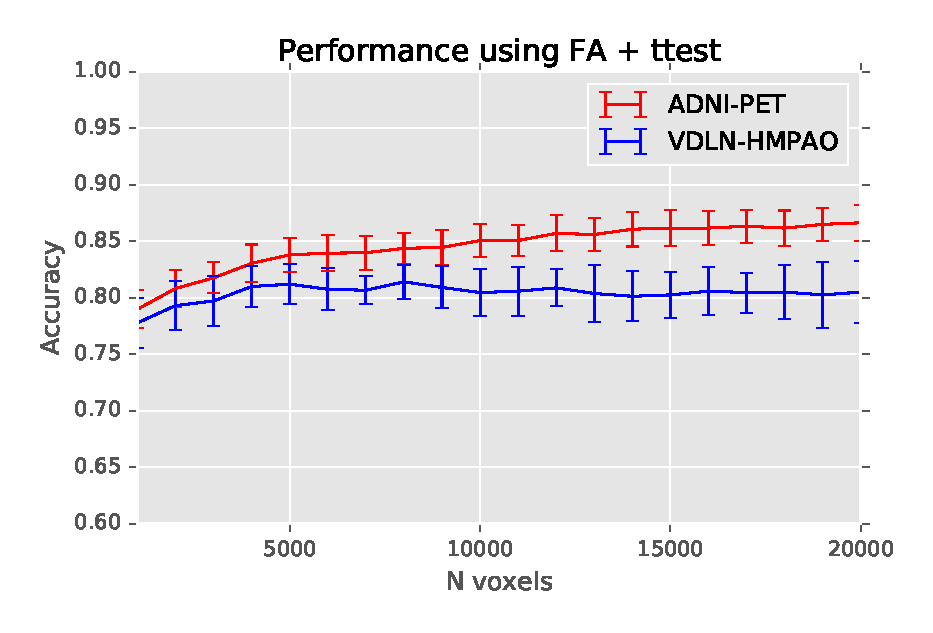
\includegraphics[width=0.49\linewidth]{Graphics/ch4/accuracyMeanSTD-FA_vsN_ttest_AD.eps}\label{fig:AD-AV-FA-TTEST-VSN}}
	\subfloat[]{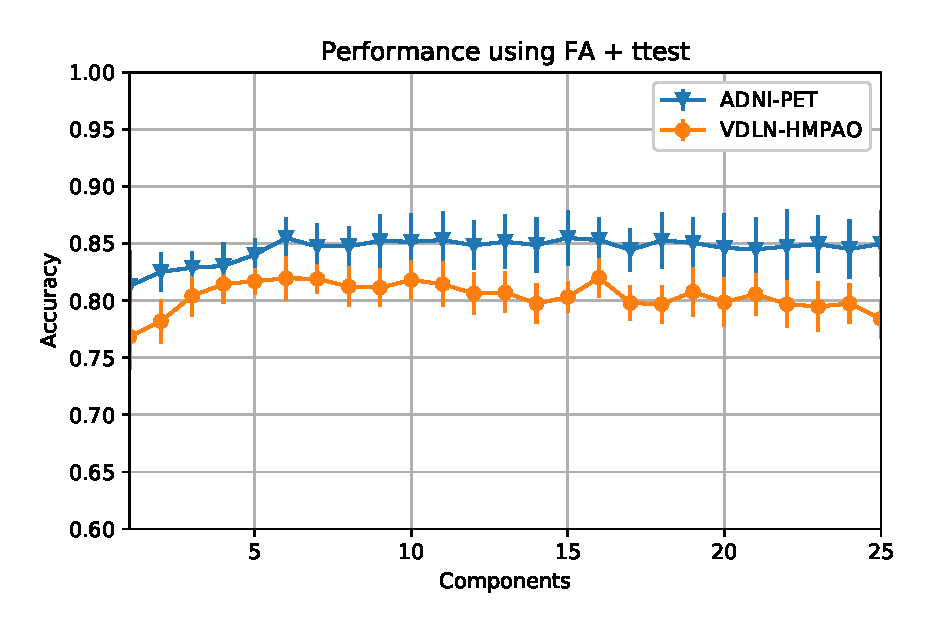
\includegraphics[width=0.49\linewidth]{Graphics/ch4/accuracyMeanSTD-FA_vsK_ttest_AD.eps}\label{fig:AD-AV-FA-TTEST-VSK}}
	
	\subfloat[]{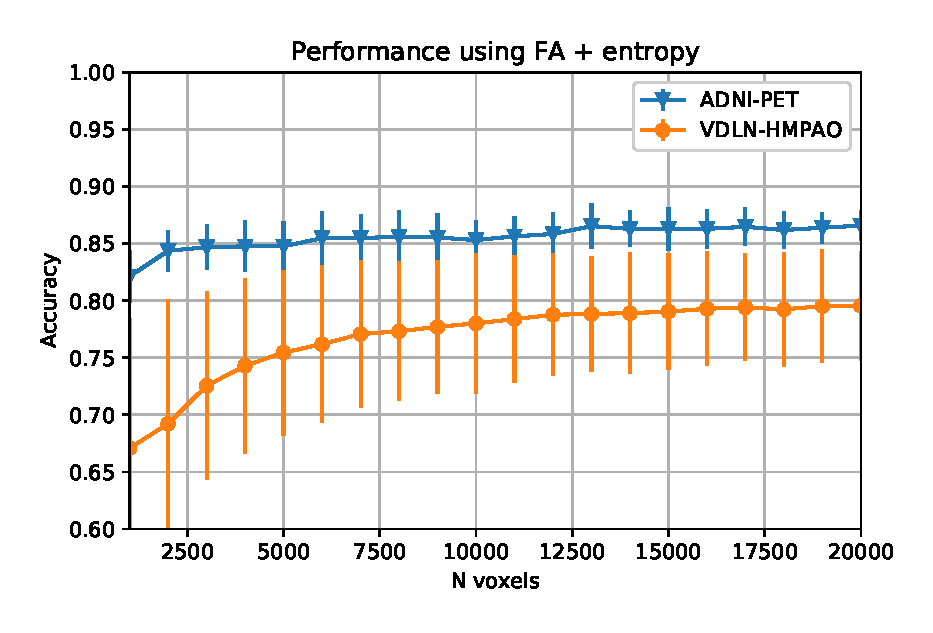
\includegraphics[width=0.49\linewidth]{Graphics/ch4/accuracyMeanSTD-FA_vsN_entropy_AD.eps}\label{fig:AD-AV-FA-ENTROPY-VSN}}
	\subfloat[]{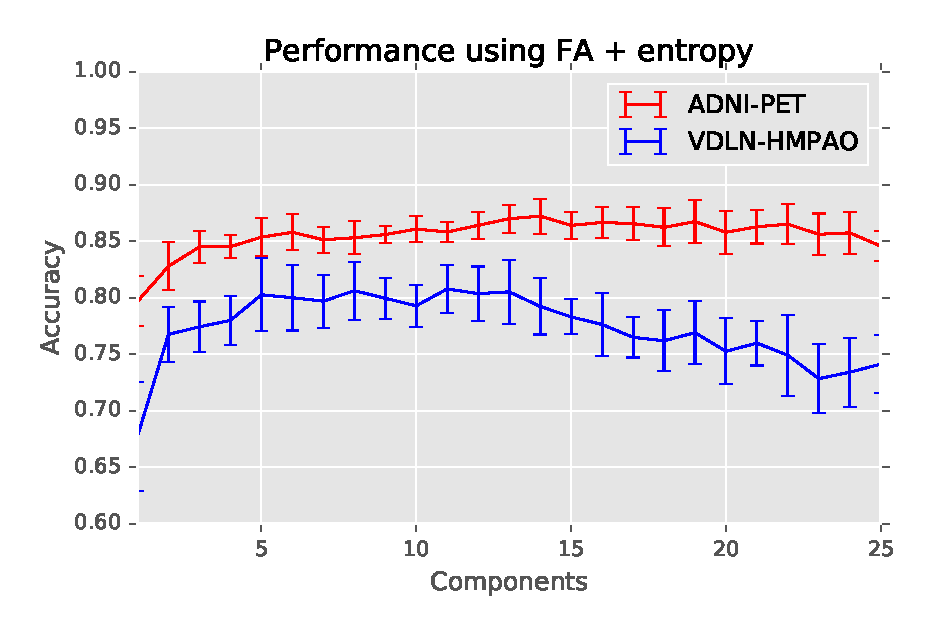
\includegraphics[width=0.49\linewidth]{Graphics/ch4/accuracyMeanSTD-FA_vsK_entropy_AD.eps}\label{fig:AD-AV-FA-ENTROPY-VSK}}
	
	\subfloat[]{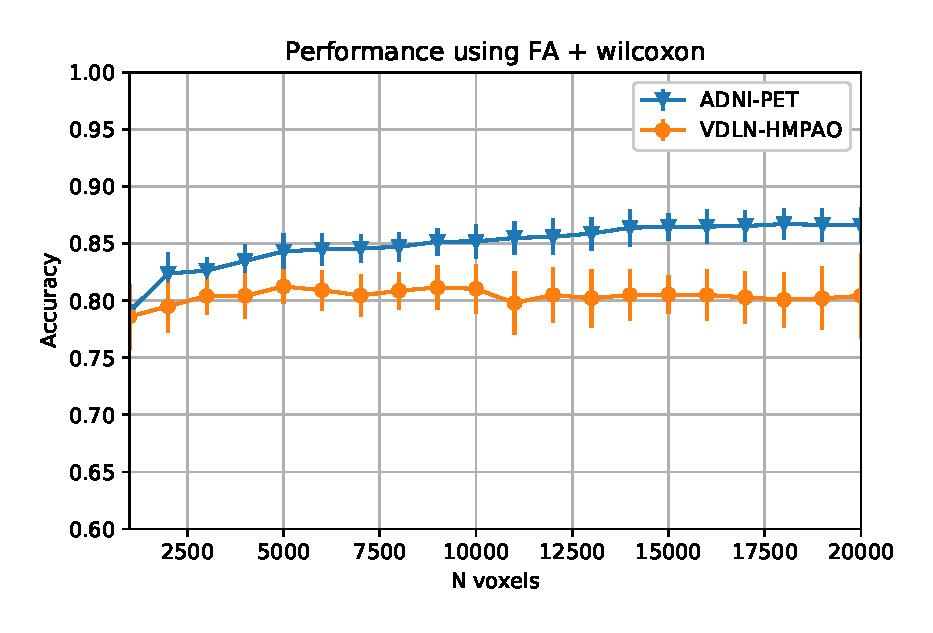
\includegraphics[width=0.49\linewidth]{Graphics/ch4/accuracyMeanSTD-FA_vsN_wilcoxon_AD.eps}\label{fig:AD-AV-FA-WILCOXON-VSN}}
	\subfloat[]{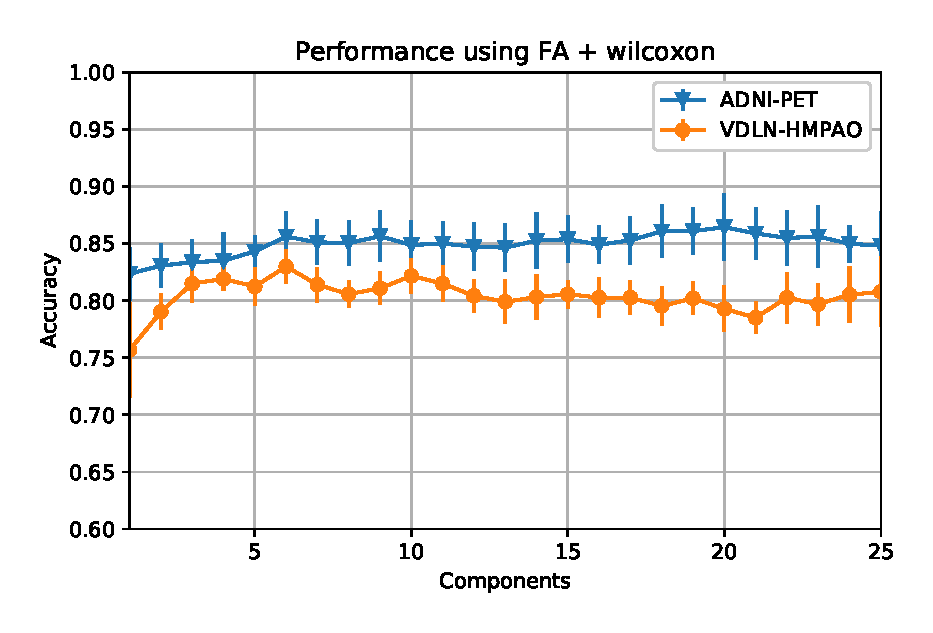
\includegraphics[width=0.49\linewidth]{Graphics/ch4/accuracyMeanSTD-FA_vsK_wilcoxon_AD.eps}\label{fig:AD-AV-FA-WILCOXON-VSK}}
	
	\caption{Average performance and standard deviation of the proposed system using the two \ac{AD} datasets, \ac{FA} and the three feature selection criteria: $t$-test (\protect\subref{fig:AD-AV-FA-TTEST-VSN} and \protect\subref{fig:AD-AV-FA-TTEST-VSK}), relative entropy (\protect\subref{fig:PKS-AV-FA-ENTROPY-VSN} and \protect\subref{fig:AD-AV-FA-ENTROPY-VSK}) and wilcoxon (\protect\subref{fig:AD-AV-FA-WILCOXON-VSN} and \protect\subref{fig:AD-AV-FA-WILCOXON-VSK}). } 
	\label{fig:accuracyMeanFA-AD}
\end{figure}

We can observe that the results are always better when using the ADNI-PET dataset than with the VDLN-HMPAO, and this is especially notorious when using the relative entropy selection criterion. The performance tends to slightly increase with the number of voxels selected, but it is not the case with the number of components. By looking at figures \ref{fig:AD-AV-FA-TTEST-VSK}, \ref{fig:AD-AV-FA-ENTROPY-VSK} and \ref{fig:AD-AV-FA-WILCOXON-VSK}, it seems that a relatively small number of components (approximately 6) is enough to obtain good performance, and afterwards, the performance holds or even decreases. 

\subsubsection{Independent Component Analysis}
In this section, we compute the results of applying \ac{ICA} to the ADNI-PET and VDLN-HMPAO datasets. Figure~\ref{fig:accuracyMeanICA-AD} depicts the average accuracy over the number of voxels or the number of components respectively for the different selection criteria. 

\begin{figure}
	\centering
	\subfloat[]{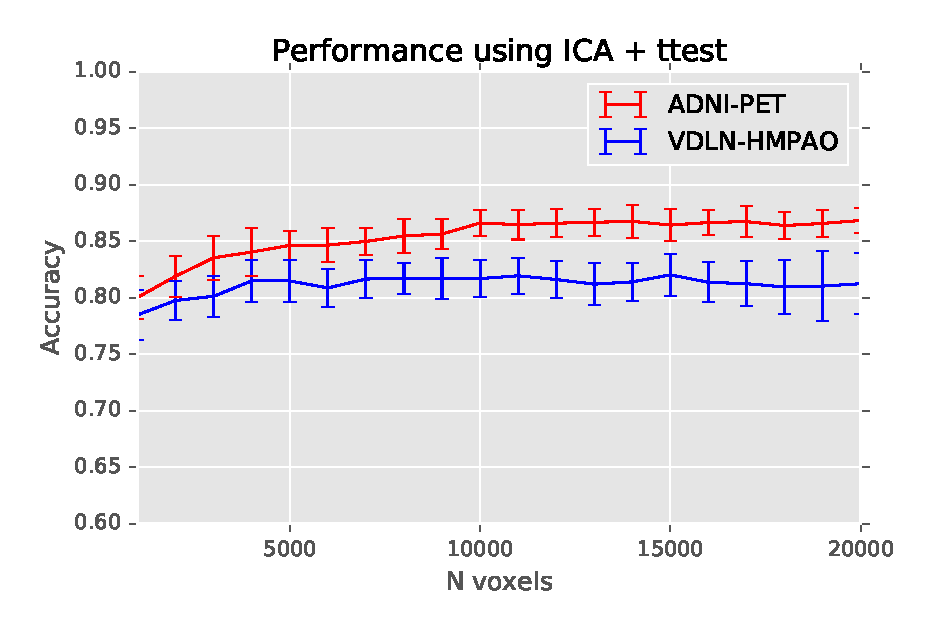
\includegraphics[width=0.49\linewidth]{Graphics/ch4/accuracyMeanSTD-ICA_vsN_ttest_AD.eps}\label{fig:AD-AV-ICA-TTEST-VSN}}
	\subfloat[]{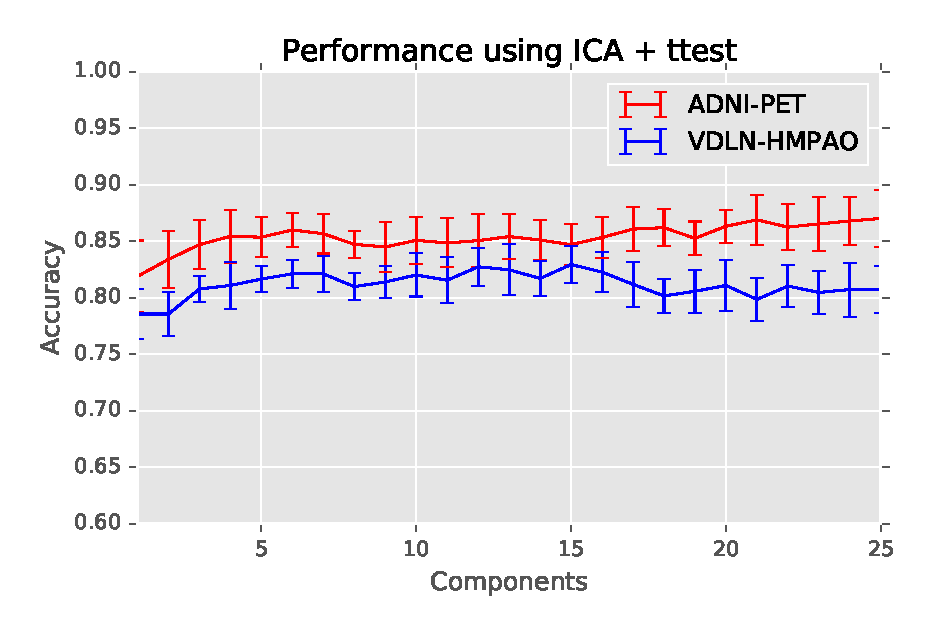
\includegraphics[width=0.49\linewidth]{Graphics/ch4/accuracyMeanSTD-ICA_vsK_ttest_AD.eps}\label{fig:AD-AV-ICA-TTEST-VSK}}
	
	\subfloat[]{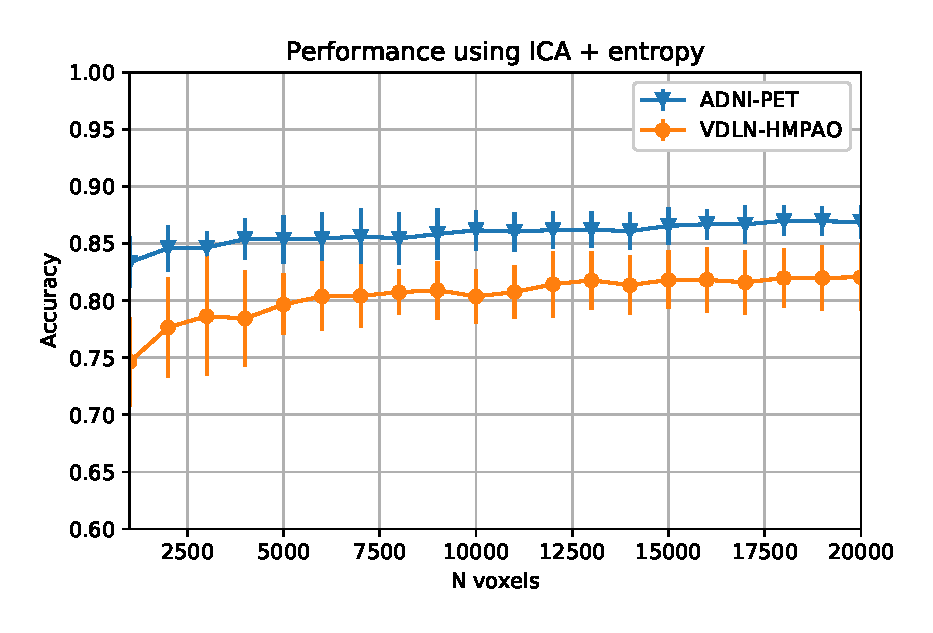
\includegraphics[width=0.49\linewidth]{Graphics/ch4/accuracyMeanSTD-ICA_vsN_entropy_AD.eps}\label{fig:AD-AV-ICA-ENTROPY-VSN}}
	\subfloat[]{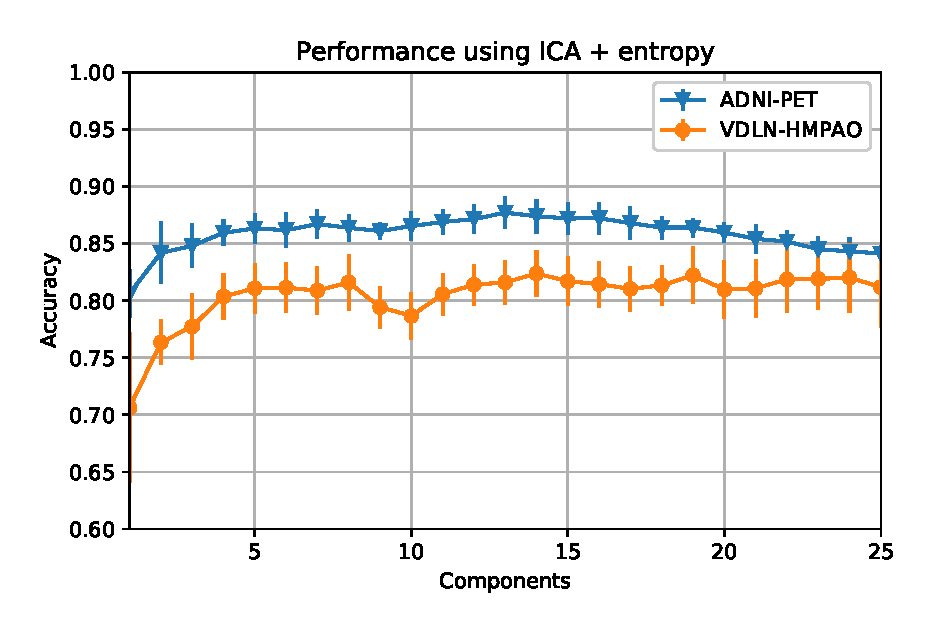
\includegraphics[width=0.49\linewidth]{Graphics/ch4/accuracyMeanSTD-ICA_vsK_entropy_AD.eps}\label{fig:AD-AV-ICA-ENTROPY-VSK}}
	
	\subfloat[]{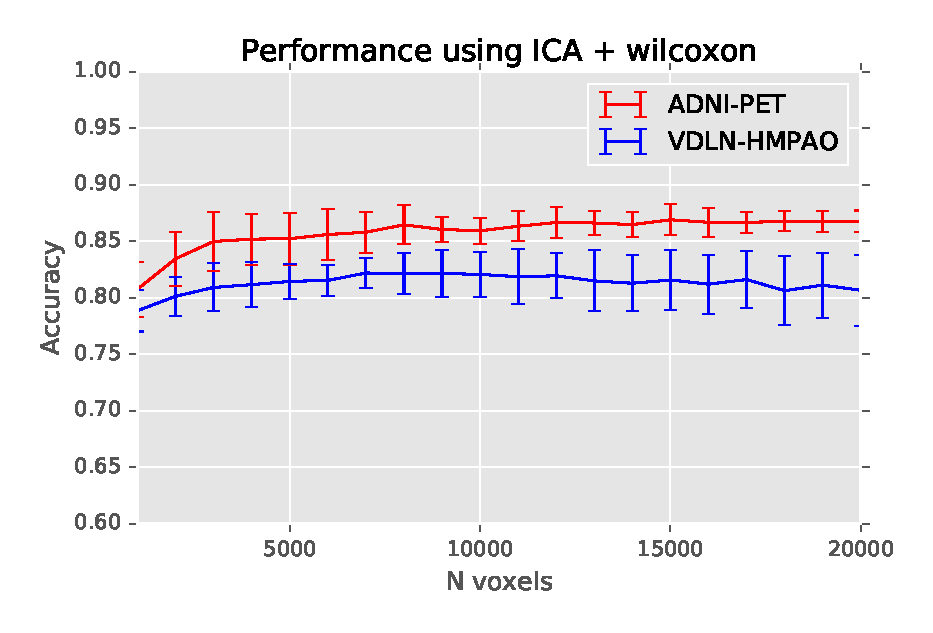
\includegraphics[width=0.49\linewidth]{Graphics/ch4/accuracyMeanSTD-ICA_vsN_wilcoxon_AD.eps}\label{fig:AD-AV-ICA-WILCOXON-VSN}}
	\subfloat[]{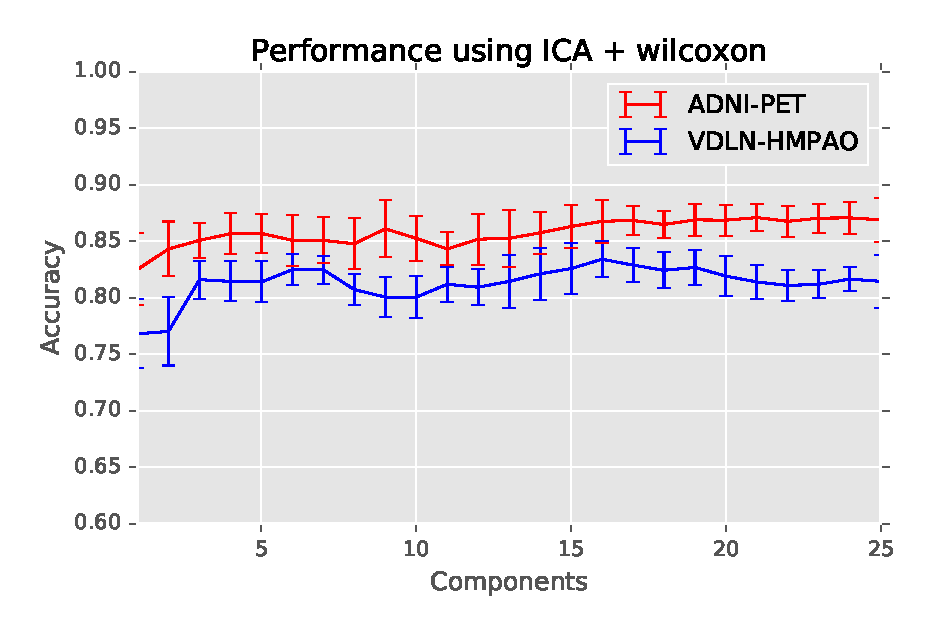
\includegraphics[width=0.49\linewidth]{Graphics/ch4/accuracyMeanSTD-ICA_vsK_wilcoxon_AD.eps}\label{fig:AD-AV-ICA-WILCOXON-VSK}}
	
	\caption{Average performance and standard deviation of the proposed system using the three \ac{AD} datasets, \ac{ICA} and the three feature selection criteria: $t$-test (\protect\subref{fig:AD-AV-ICA-TTEST-VSN} and \protect\subref{fig:AD-AV-ICA-TTEST-VSK}), relative entropy (\protect\subref{fig:AD-AV-ICA-ENTROPY-VSN} and \protect\subref{fig:AD-AV-ICA-ENTROPY-VSK}) and wilcoxon (\protect\subref{fig:AD-AV-ICA-WILCOXON-VSN} and \protect\subref{fig:AD-AV-ICA-WILCOXON-VSK}). } 
	\label{fig:accuracyMeanICA-AD}
\end{figure}

The case is similar to the one presented in Section~\ref{sec:results_FA_AD}, where the performance slightly improves when increasing the number of selected voxels. The performance is again better when using the ADNI-PET dataset than with the VDLN-HMPAO, although the behaviour is similar. 

The results change when varying the number of components. In this case, although good performance is obtained within the first 5 components in most cases, the performance does not decrease with a higher number, and sometimes increases (for example, in the case of \ac{ICA} and the $t$-test or the wilcoxon selection criteria). 

\subsubsection{At the Operation Point}
Now we focus on non-averaged values, the values for which our system is optimal: the operation point. 

\begin{figure}
	\centering
	\subfloat[]{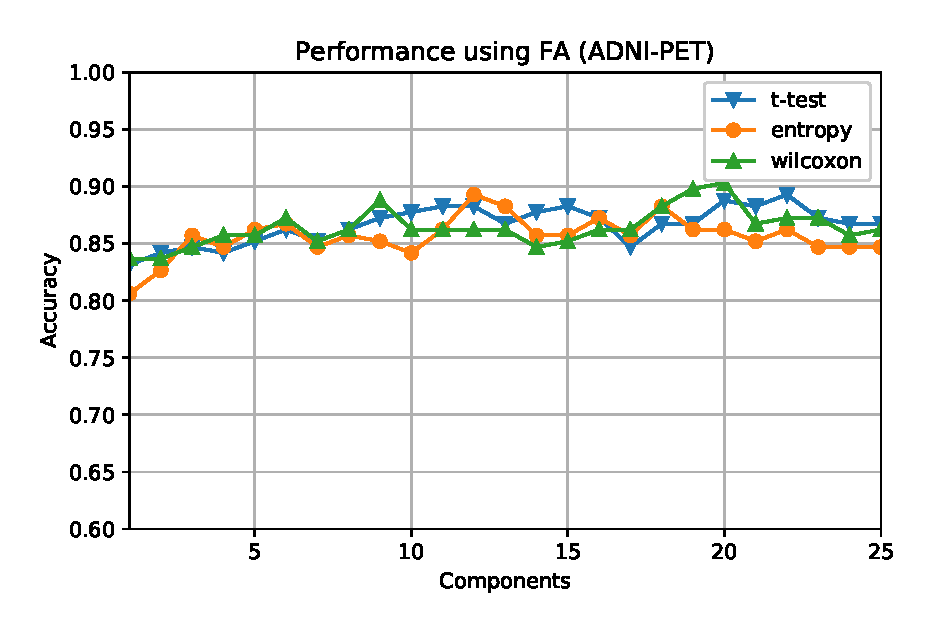
\includegraphics[width=0.49\linewidth]{Graphics/ch4/accuracyOP-FA_vsN_comparison_ADNI-PET.eps}\label{fig:ADNI-PET-FA-OP}}
	\subfloat[]{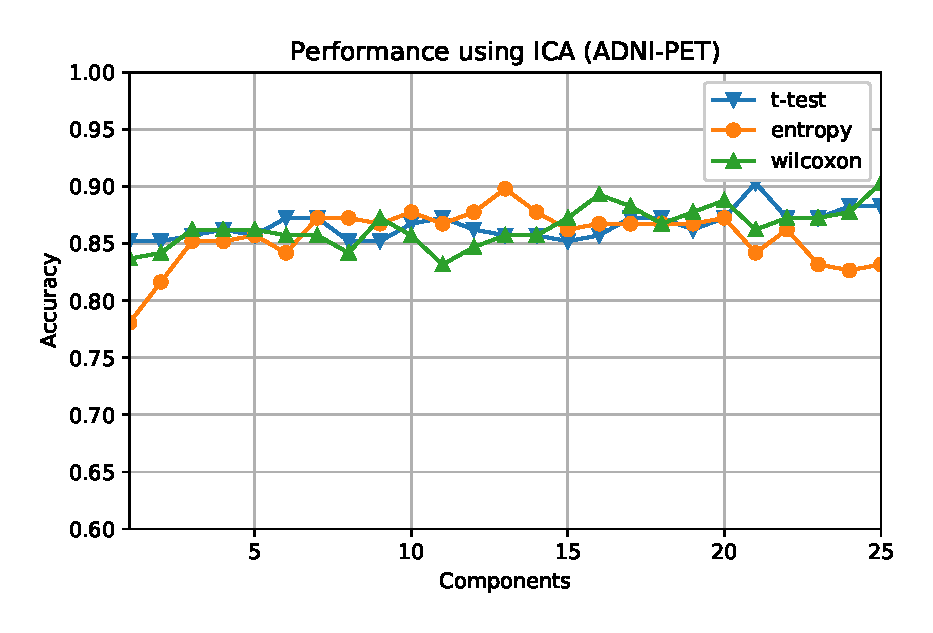
\includegraphics[width=0.49\linewidth]{Graphics/ch4/accuracyOP-ICA_vsN_comparison_ADNI-PET.eps}\label{fig:ADNI-PET-ICA-OP}}
	
	\subfloat[]{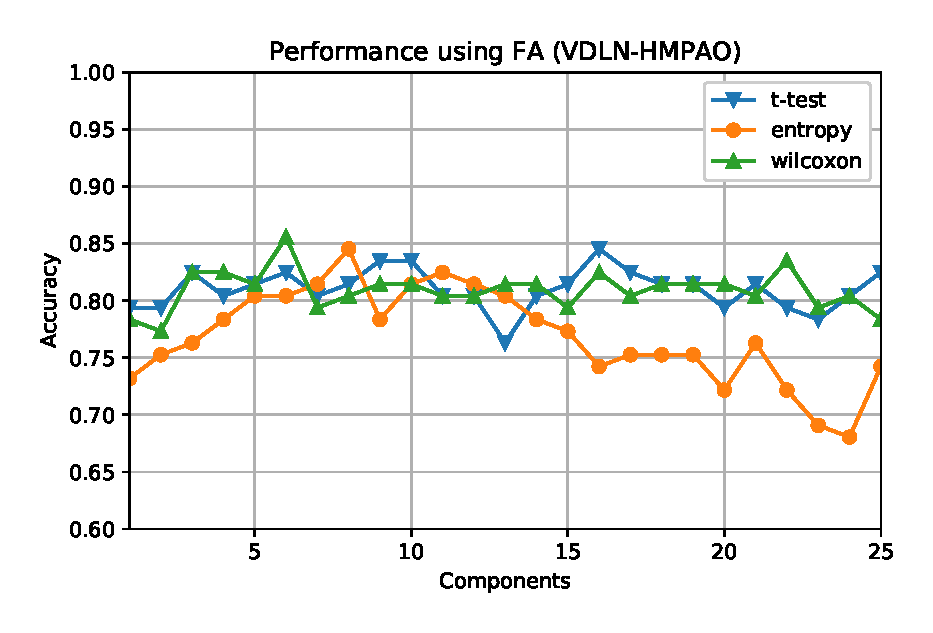
\includegraphics[width=0.49\linewidth]{Graphics/ch4/accuracyOP-FA_vsN_comparison_VDLN-HMPAO.eps}\label{fig:VDLN-HMPAO-FA-OP}}
	\subfloat[]{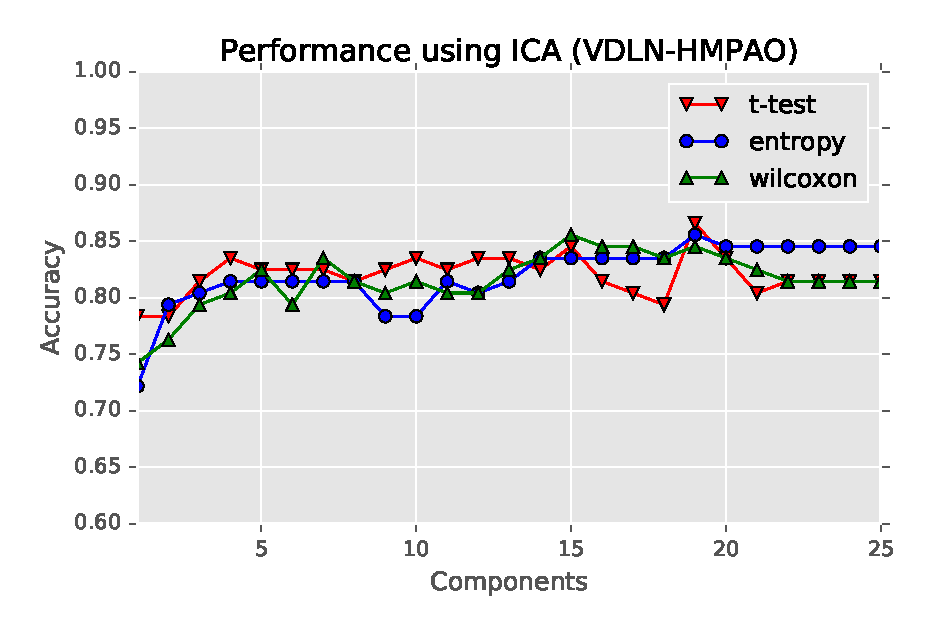
\includegraphics[width=0.49\linewidth]{Graphics/ch4/accuracyOP-ICA_vsN_comparison_VDLN-HMPAO.eps}\label{fig:VDLN-HMPAO-ICA-OP}}
	
	\caption{Performance of the proposed system using the two \ac{AD} datasets: ADNI-PET and VDLN-HMPAO at the operation point, and how they vary over the number of components used in the decomposition. } 
	\label{fig:accuracyOP-AD}
\end{figure}


\begin{table}
	\myfloatalign
	\begin{tabularx}{\linewidth}{Xllccc}
		\tableheadline{DB} & \tableheadline{Dec.} & \tableheadline{Criterion} & \tableheadline{Accuracy} & \tableheadline{Sensitivity} & \tableheadline{Specificity}\\
		\toprule
		\multirow{6}{1.7cm}{ADNI- PET} & \multirow{3}{*}{\ac{FA}} & t-test & $ 0.893 \pm 0.074 $ & $ 0.886 \pm 0.119 $ & $ 0.901 \pm 0.101 $ \\
		&  & entropy & $ 0.893 \pm 0.074 $ & $ 0.894 \pm 0.092 $ & $ 0.891 \pm 0.088 $ \\
		&  & wilcoxon & $ 0.903 \pm 0.066 $ & $ 0.917 \pm 0.079 $ & $ 0.891 \pm 0.082 $ \\
		\cline{2-6}
		& \multirow{3}{*}{\ac{ICA}} & t-test & $ 0.903 \pm 0.071 $ & $ 0.893 \pm 0.100 $ & $ 0.910 \pm 0.107 $ \\
		&  & entropy & $ 0.898 \pm 0.059 $ & $ 0.917 \pm 0.088 $ & $ 0.881 \pm 0.084 $ \\
		&  & wilcoxon & $ 0.903 \pm 0.066 $ & $ 0.906 \pm 0.097 $ & $ 0.901 \pm 0.094 $ \\ \midrule
		\multirow{6}{1.7cm}{VDLN- HMPAO} & \multirow{3}{*}{\ac{FA}} & t-test & $ 0.845 \pm 0.102 $ & $ 0.843 \pm 0.158 $ & $ 0.855 \pm 0.140 $ \\
		&  & entropy & $ 0.845 \pm 0.052 $ & $ 0.893 \pm 0.146 $ & $ 0.785 \pm 0.163 $ \\
		&  & wilcoxon & $ 0.856 \pm 0.084 $ & $ 0.857 \pm 0.137 $ & $ 0.855 \pm 0.151 $ \\
		\cline{2-6}
		& \multirow{3}{*}{\ac{ICA}} & t-test & $ 0.866 \pm 0.085 $ & $ 0.873 \pm 0.144 $ & $ 0.855 \pm 0.154 $ \\
		&  & entropy & $ 0.856 \pm 0.101 $ & $ 0.853 \pm 0.138 $ & $ 0.855 \pm 0.151 $ \\
		&  & wilcoxon & $ 0.856 \pm 0.086 $ & $ 0.857 \pm 0.156 $ & $ 0.855 \pm 0.160 $ \\
		\bottomrule
	\end{tabularx}
	\caption{Accuracy, sensitivity, specificity, and their standard deviation at the operation point for each method and its corresponding feature selection criterion, using two \protect\ac{AD} datasets. }
	\label{tab:featureAD}
\end{table}
\FloatBarrier
\subsection{Parkinson's Disease}


\subsubsection{Factor Analysis}
\begin{figure}
	\centering
	\subfloat[]{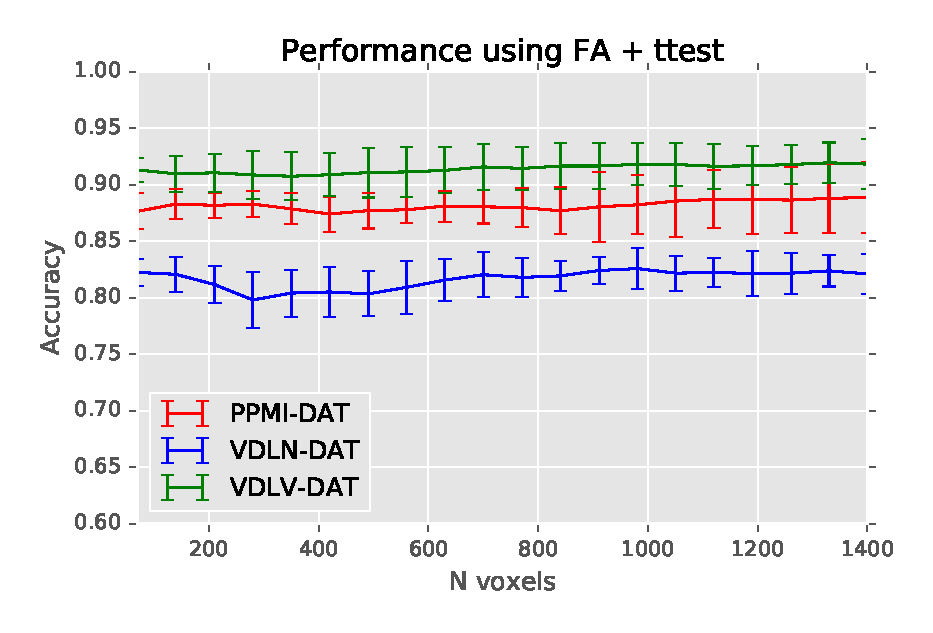
\includegraphics[width=0.49\linewidth]{Graphics/ch4/accuracyMeanSTD-FA_vsN_ttest_PKS.eps}\label{fig:PKS-AV-FA-TTEST-VSN}}
	\subfloat[]{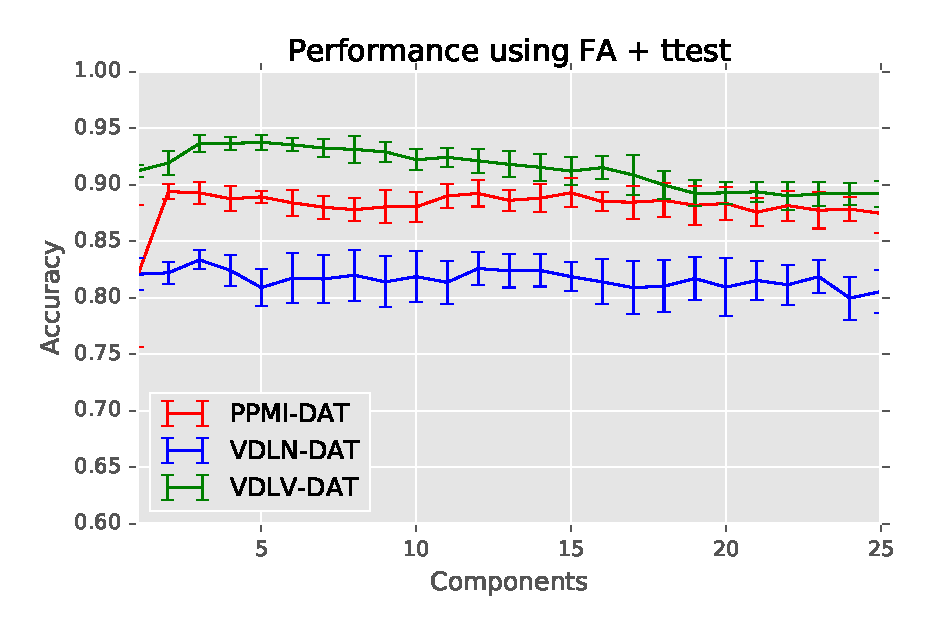
\includegraphics[width=0.49\linewidth]{Graphics/ch4/accuracyMeanSTD-FA_vsK_ttest_PKS.eps}\label{fig:PKS-AV-FA-TTEST-VSK}}
	
	\subfloat[]{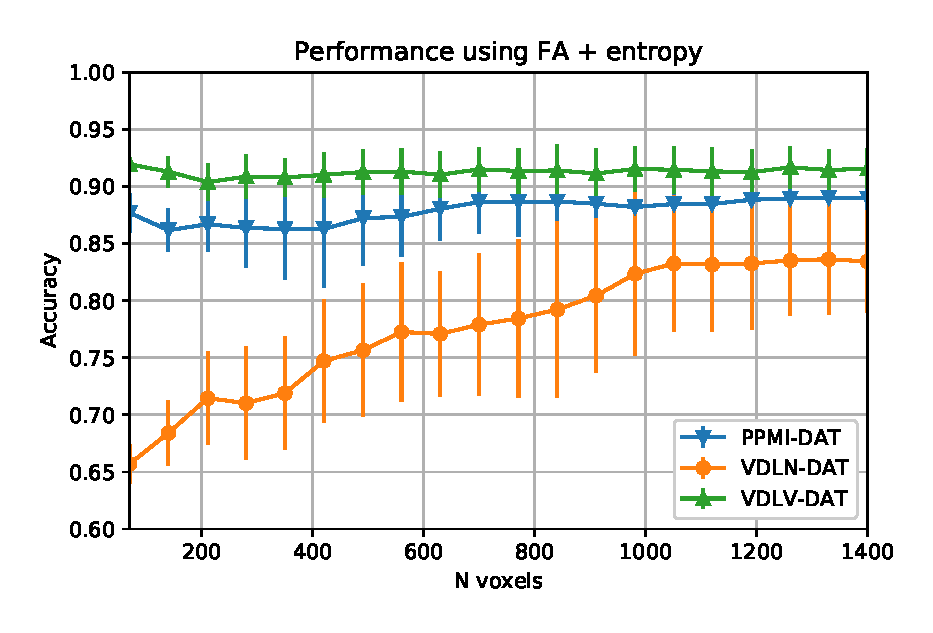
\includegraphics[width=0.49\linewidth]{Graphics/ch4/accuracyMeanSTD-FA_vsN_entropy_PKS.eps}\label{fig:PKS-AV-FA-ENTROPY-VSN}}
	\subfloat[]{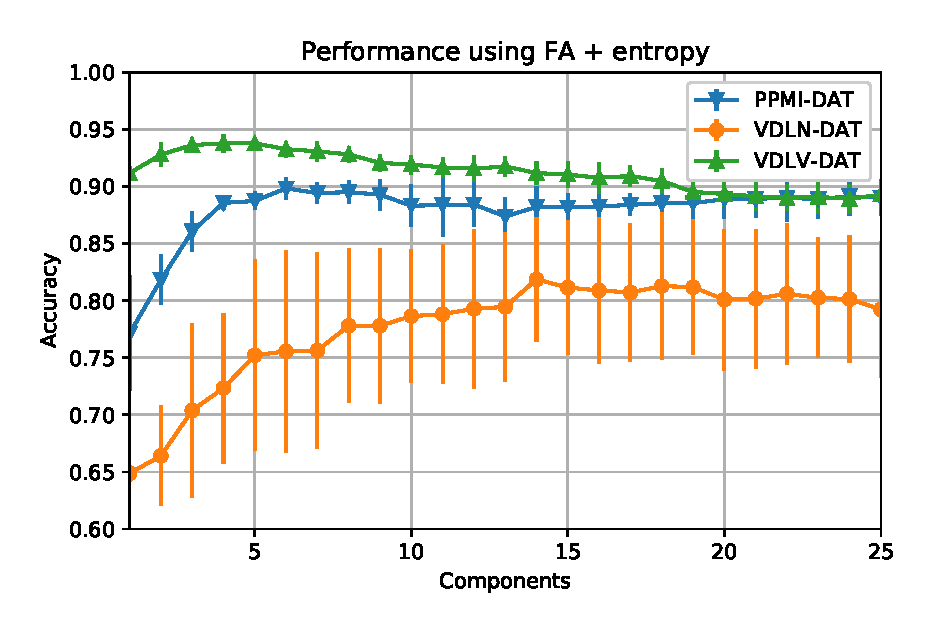
\includegraphics[width=0.49\linewidth]{Graphics/ch4/accuracyMeanSTD-FA_vsK_entropy_PKS.eps}\label{fig:PKS-AV-FA-ENTROPY-VSK}}
	
	\subfloat[]{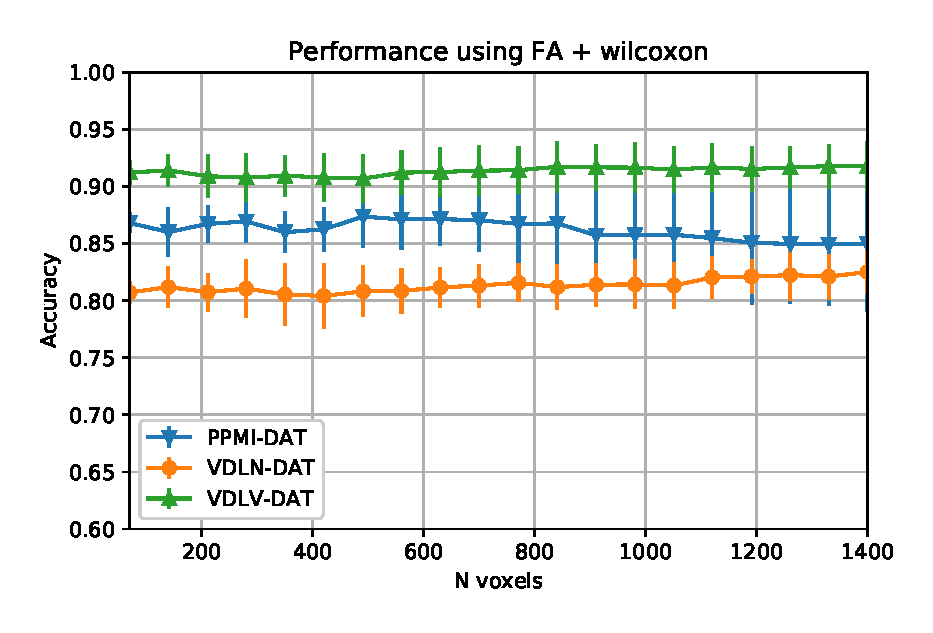
\includegraphics[width=0.49\linewidth]{Graphics/ch4/accuracyMeanSTD-FA_vsN_wilcoxon_PKS.eps}\label{fig:PKS-AV-FA-WILCOXON-VSN}}
	\subfloat[]{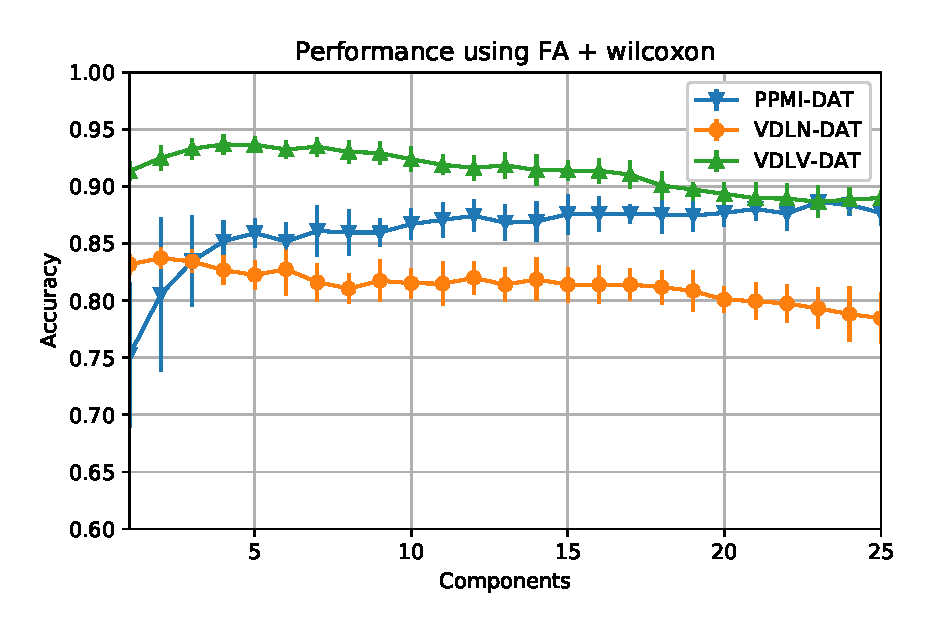
\includegraphics[width=0.49\linewidth]{Graphics/ch4/accuracyMeanSTD-FA_vsK_wilcoxon_PKS.eps}\label{fig:PKS-AV-FA-WILCOXON-VSK}}
	
	\caption{Average performance and standard deviation of the proposed system using the three \ac{PKS} datasets, \ac{FA} and the three feature selection criteria: $t$-test (\protect\subref{fig:PKS-AV-FA-TTEST-VSN} and \protect\subref{fig:PKS-AV-FA-TTEST-VSK}), relative entropy (\protect\subref{fig:PKS-AV-FA-ENTROPY-VSN} and \protect\subref{fig:PKS-AV-FA-ENTROPY-VSK}) and wilcoxon (\protect\subref{fig:PKS-AV-FA-WILCOXON-VSN} and \protect\subref{fig:PKS-AV-FA-WILCOXON-VSK}). } 
	\label{fig:accuracyMeanFA-PKS}
\end{figure}

\subsubsection{Independent Component Analysis}
\begin{figure}
	\subfloat[]{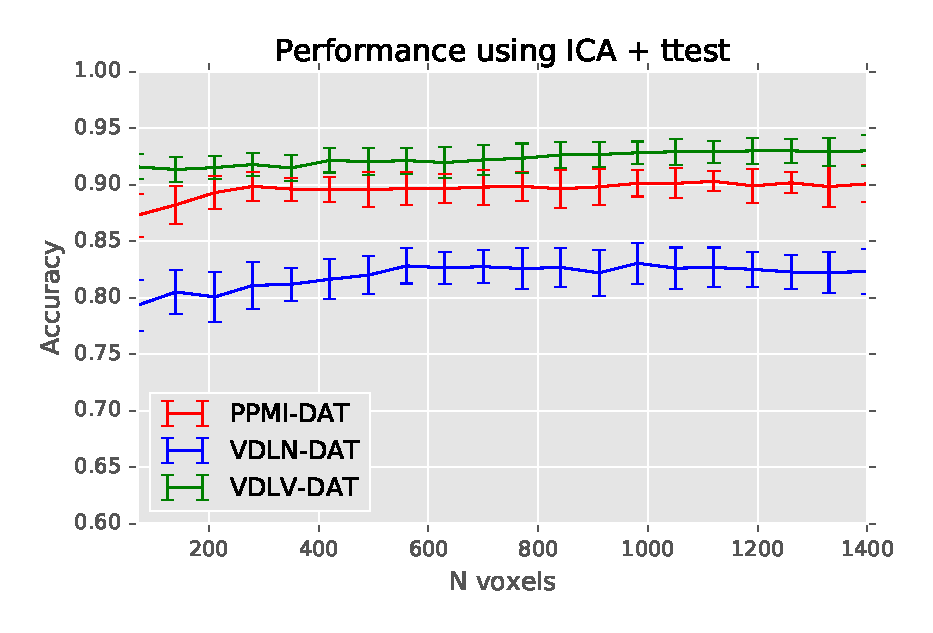
\includegraphics[width=0.49\linewidth]{Graphics/ch4/accuracyMeanSTD-ICA_vsN_ttest_PKS.eps}\label{fig:PKS-AV-ICA-TTEST-VSN}}
	\subfloat[]{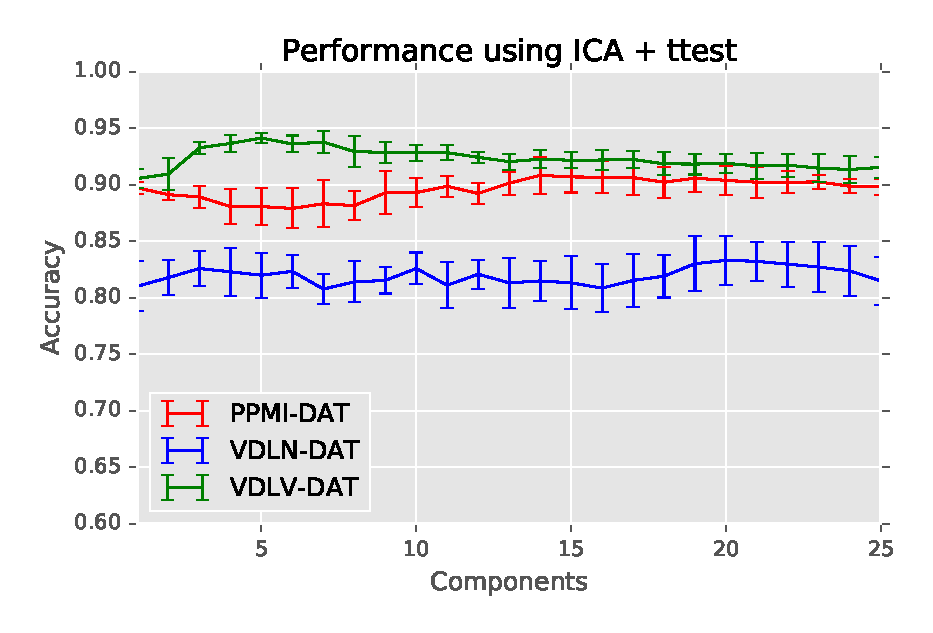
\includegraphics[width=0.49\linewidth]{Graphics/ch4/accuracyMeanSTD-ICA_vsK_ttest_PKS.eps}\label{fig:PKS-AV-ICA-TTEST-VSK}}
	
	\subfloat[]{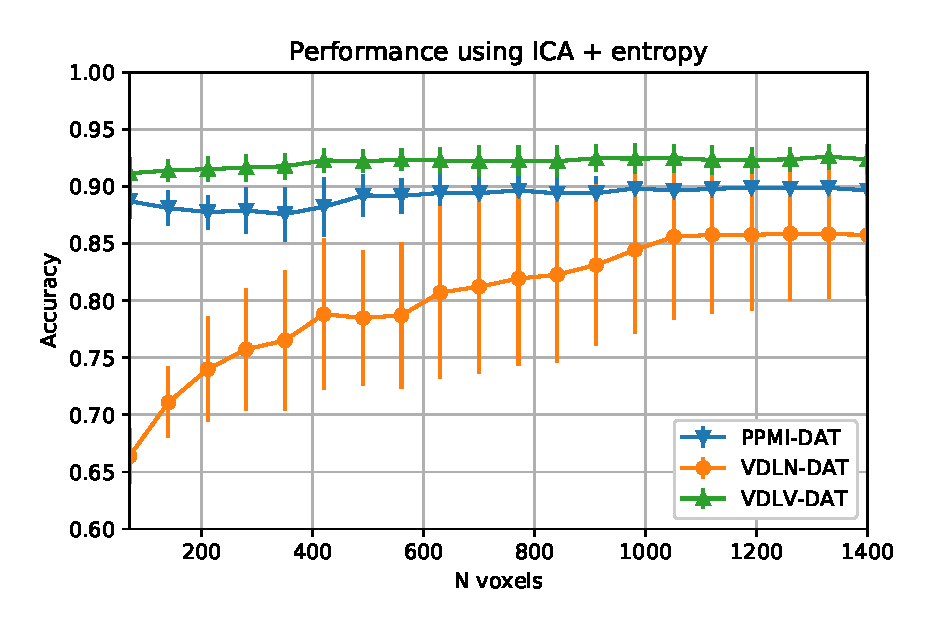
\includegraphics[width=0.49\linewidth]{Graphics/ch4/accuracyMeanSTD-ICA_vsN_entropy_PKS.eps}\label{fig:PKS-AV-ICA-ENTROPY-VSN}}
	\subfloat[]{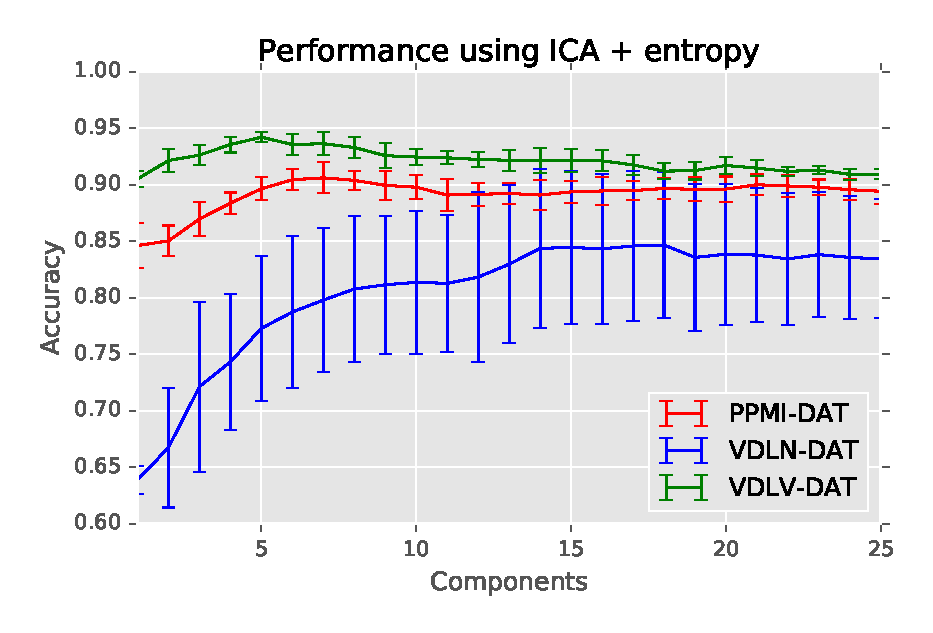
\includegraphics[width=0.49\linewidth]{Graphics/ch4/accuracyMeanSTD-ICA_vsK_entropy_PKS.eps}\label{fig:PKS-AV-ICA-ENTROPY-VSK}}
	
	\subfloat[]{\includegraphics[width=0.49\linewidth]{Graphics/ch4/accuracyMeanSTD-ICA_vsN_wilcoxon_PKS.eps}\label{fig:PKS-AV-ICA-WILCOXON-VSN}}
	\subfloat[]{\includegraphics[width=0.49\linewidth]{Graphics/ch4/accuracyMeanSTD-ICA_vsK_wilcoxon_PKS.eps}\label{fig:PKS-AV-ICA-WILCOXON-VSK}}
	
	\caption{Average performance and standard deviation of the proposed system using the three \ac{PKS} datasets, \ac{ICA} and the three feature selection criteria: $t$-test (\protect\subref{fig:PKS-AV-ICA-TTEST-VSN} and \protect\subref{fig:PKS-AV-ICA-TTEST-VSK}), relative entropy (\protect\subref{fig:PKS-AV-ICA-ENTROPY-VSN} and \protect\subref{fig:PKS-AV-ICA-ENTROPY-VSK}) and wilcoxon (\protect\subref{fig:PKS-AV-ICA-WILCOXON-VSN} and \protect\subref{fig:PKS-AV-ICA-WILCOXON-VSK}). } 
	\label{fig:accuracyMeanICA-PKS}
\end{figure}


\subsubsection{At the Operation Point}

\begin{figure}
	\subfloat[]{\includegraphics[width=0.49\linewidth]{Graphics/ch4/accuracyOP-FA_vsN_comparison_PPMI-DAT.eps}\label{fig:PPMI-DAT-FA-OP}}
	\subfloat[]{\includegraphics[width=0.49\linewidth]{Graphics/ch4/accuracyOP-ICA_vsN_comparison_PPMI-DAT.eps}\label{fig:PPMI-DAT-ICA-OP}}
	
	\subfloat[]{\includegraphics[width=0.49\linewidth]{Graphics/ch4/accuracyOP-FA_vsN_comparison_VDLN-DAT.eps}\label{fig:VDLN-DAT-FA-OP}}
	\subfloat[]{\includegraphics[width=0.49\linewidth]{Graphics/ch4/accuracyOP-ICA_vsN_comparison_VDLN-DAT.eps}\label{fig:VDLN-DAT-ICA-OP}}
	
	\subfloat[]{\includegraphics[width=0.49\linewidth]{Graphics/ch4/accuracyOP-FA_vsN_comparison_VDLV-DAT.eps}\label{fig:VDLV-DAT-FA-OP}}
	\subfloat[]{\includegraphics[width=0.49\linewidth]{Graphics/ch4/accuracyOP-ICA_vsN_comparison_VDLV-DAT.eps}\label{fig:VDLV-DAT-ICA-OP}}
	
	\caption{Performance of the proposed system using the two \ac{PKS} datasets: PPMI-DAT, VDLN-DAT and VDLV-DAT at the operation point, and how they vary over the number of components used in the decomposition. } 
	\label{fig:accuracyOP-PKS}
\end{figure}


\begin{table}
	\begin{tabularx}{\linewidth}{Xllccc}
		\tableheadline{DB} & \tableheadline{Dec.} & \tableheadline{Criterion} & \tableheadline{Accuracy} & \tableheadline{Sensitivity} & \tableheadline{Specificity}\\
		\toprule
		\multirow{6}{1.7cm}{VDLN-DAT} & \multirow{3}{*}{\ac{FA}} & t-test & $ 0.856 \pm 0.111 $ & $ 0.887 \pm 0.178 $ & $ 0.795 \pm 0.164 $ \\
		&  & entropy & $ 0.890 \pm 0.098 $ & $ 0.875 \pm 0.118 $ & $ 0.910 \pm 0.116 $ \\
		&  & wilcoxon & $ 0.864 \pm 0.070 $ & $ 0.916 \pm 0.114 $ & $ 0.780 \pm 0.183 $ \\
		\cline{2-6}
		& \multirow{3}{*}{\ac{ICA}} & t-test & $ 0.864 \pm 0.101 $ & $ 0.873 \pm 0.174 $ & $ 0.840 \pm 0.166 $ \\
		&  & entropy & $ 0.907 \pm 0.075 $ & $ 0.889 \pm 0.124 $ & $ 0.935 \pm 0.131 $ \\
		&  & wilcoxon & $ 0.873 \pm 0.108 $ & $ 0.859 \pm 0.181 $ & $ 0.890 \pm 0.151 $ \\
		\midrule
		\multirow{6}{1.7cm}{VDLV-DAT} & \multirow{3}{*}{\ac{FA}} & t-test & $ 0.957 \pm 0.033 $ & $ 0.940 \pm 0.066 $ & $ 0.973 \pm 0.065 $ \\
		&  & entropy & $ 0.952 \pm 0.037 $ & $ 0.940 \pm 0.066 $ & $ 0.964 \pm 0.064 $ \\
		&  & wilcoxon & $ 0.957 \pm 0.033 $ & $ 0.940 \pm 0.066 $ & $ 0.973 \pm 0.065 $ \\
		\cline{2-6}
		& \multirow{3}{*}{\ac{ICA}} & t-test & $ 0.952 \pm 0.037 $ & $ 0.940 \pm 0.066 $ & $ 0.964 \pm 0.064 $ \\
		&  & entropy & $ 0.947 \pm 0.045 $ & $ 0.940 \pm 0.066 $ & $ 0.955 \pm 0.076 $ \\
		&  & wilcoxon & $ 0.952 \pm 0.037 $ & $ 0.940 \pm 0.066 $ & $ 0.964 \pm 0.064 $ \\
		\midrule
		\multirow{6}{1.7cm}{PPMI-DAT} & \multirow{3}{*}{\ac{FA}} & t-test & $ 0.917 \pm 0.037 $ & $ 0.918 \pm 0.095 $ & $ 0.918 \pm 0.091 $ \\
		&  & entropy & $ 0.917 \pm 0.060 $ & $ 0.918 \pm 0.076 $ & $ 0.921 \pm 0.120 $ \\
		&  & wilcoxon & $ 0.912 \pm 0.056 $ & $ 0.927 \pm 0.098 $ & $ 0.889 \pm 0.102 $ \\
		\cline{2-6}
		& \multirow{3}{*}{\ac{ICA}} & t-test & $ 0.917 \pm 0.056 $ & $ 0.900 \pm 0.095 $ & $ 0.948 \pm 0.109 $ \\
		&  & entropy & $ 0.928 \pm 0.055 $ & $ 0.909 \pm 0.091 $ & $ 0.961 \pm 0.090 $ \\
		&  & wilcoxon & $ 0.912 \pm 0.070 $ & $ 0.909 \pm 0.100 $ & $ 0.920 \pm 0.118 $ \\
		\bottomrule
		\end{tabularx}
		\caption{Accuracy, sensitivity, specificity, and their standard deviation at the operation point for each method and its corresponding feature selection criterion, using three \protect\ac{PKS} datasets }
		\label{tab:featurePKS}
\end{table}

\section{Discussion}

\cleardoublepage
\ctparttext{The first approach to reduce the small sample size problem in neuroimaging studies is based on reducing the number of features .}
\part{Feature Size Reduction}
%\addtocontents{toc}{\protect\clearpage} % <--- just debug stuff, ignore
%************************************************
\chapter{Texture Features}\label{ch:texture}
%************************************************
\section{Introduction}
Texture is a household word outside image processing or related fields. However, in that context, it lacks a definition that allow us to measure and quantify it. Patter recognition provides us with a mathematical definition that allow us to use texture as a feature in our \ac{CAD} systems. 

Texture analysis is defined as any procedure by which we can quantify and classify the spatial variation of intensity throughout an image. In neuroimaging, texture has been widely used in segmentation (tissue classification) of \ac{MRI} images \cite{Saeed2002,Alejo2003,Wang2009}, although there exist a number of works using it for feature extraction in \ac{CAD}-like systems, like the works in \cite{kovalev2001three,sikio2015mr}, or our work on \ac{PKS} feature extraction \cite{Martinez-Murcia2013266,martinez2014parametrization}. 

Texture features can be classified in first, second and higher order analysis, depending on the number of variables used. First order statistics \cite{Martinez-Murcia2016b} are the most basic form of texture analysis, computing values such as average, variance or histogram of voxel intensity values \cite{Srinivasan2008}. 

The most popular form, with a very developed theoretical background, is second-order statistical texture analysis. This particular form is based on the probability of finding a pair of similar intensities at a certain distance and orientation of a certain image. From these probabilities, many measures can be derived, being the most popular the Haralick texture analysis \cite{Haralick73}. 

\begin{figure}[htp]
\centering
\includegraphics[width=0.9\linewidth]{Graphics/ch5/01-flowdiagram}
\caption[Schema of the proposed Texture-based CAD system.]{Schema of the proposed Texture-based \ac{CAD} system, including an optional feature selection block.}
\label{fig:textureCAD}
\end{figure}

In this work we have used Haralick texture analysis to extract features from DaTSCAN images and perform an automatic diagnosis of \ac{PD}. It follows the pipeline depicted at Figure~\ref{fig:textureCAD}, as in \cite{Martinez-Murcia2013266,martinez2014parametrization}. First we will provide an introduction to the methodology followed at Section~\ref{sec:methodsCh5}, including the volume selection tools, the Haralick texture analysis and the experiments used to validate the system. Later, in Section~\ref{sec:ch5results} we define the experiments and show their results. Finally, at Section~\ref{sec:ch5discuss} we discuss the implications of this systems and the evaluation results of our texture-based \ac{CAD} system.

\section{Methodology}\label{sec:methodsCh5}

\subsection{Volume selection}\label{sec:volume}
Even the registered DaTSCAN images contain many voxels that are outside the brain. Therefore, to obtain a more robust estimation of the texture, it would be desirable to perform the computation of the features on subvolumes of those images (or subimages) that contain only voxels inside the brain. Many strategies can be performed for this, for example, force the computation of the \ac{GLCM} to ignore background voxels. 

In this work, we opted for extracting a subvolume which contains only voxels higher than a certain intensity threshold $I_{th}$, which should be specified. To do so, we obtain the maximum and minimum coordinates for which $\mathbf{I}$ is higher than the threshold: 
\begin{align}
	p_{x,min} & = \argmin_x \left( \mathbf{I} > I_{th} \right)\\
	p_{x,max} & = \argmax_x \left( \mathbf{I} > I_{th} \right)
\end{align}

And we do the same for the $y$ and $z$ axis of the array. Once this is computed, we can select the volume by: 

\begin{equation}
	\mathbf{I}_{sub} = \mathbf{I}[p_{x,min}:p_{x,max}, p_{y,min}:p_{y,max}, p_{z,min}:p_{z,max}]
\end{equation}

The resulting subvolume $\mathbf{I}_{sub}$ is the minimum box-shaped volume containing all the values for which $\mathbf{I}>I_{th}$, which allow us to select a $I_{th}$ so that only the regions of interest are contained within. 

Different subimages and sizes are obtained when applying different $I_{th}$ In Figure~\ref{fig:comparisonIth} we depict a comparison between the resulting images for $I_{th} = [0.25, 0.30, 0.35]$. 

\begin{figure}
	\centering
	\includegraphics[width=0.90\columnwidth]{Graphics/ch5/comparisonIth.eps}
	\caption[Comparison of the different $I_{th}$ values.]{Comparison of the different $I_{th}$ values for a random subject extracted from the PPMI database.}
	\label{fig:comparisonIth}
\end{figure}

\subsection{Haralick Texture Analysis}\label{sec:haralick}
\subsubsection{Gray Level Co-occurrence Matrix}
%Que son las matriz de coocurrencia y las texture features
The Haralick texture analysis is based on the computation of a \acf{GLCM}, which is a form of evaluating second-order texture statistics. This matrix is a summary of the probabilities of finding a pair of similar grey levels at a certain distance and in a certain direction. 

The combination of the unitary vector dimension and the distance defines the offset $\Delta=(d_x,d_y,d_z)$, whose norm is the distance $d$ and is defined in a given spatial direction. In this work, we use a three-dimensional approach to the computation of the \ac{GLCM}, based on \cite{Philips2008}, that uses thirteen spatial directions to generalize the standard 2D \ac{GLCM} to 3D. These offset define different angles and are used to get some degree of rotational invariance \cite{Philips2008}. 

Medical images have different number precision, which can vary from regular 8bit integers (256 values) to the type float64 ($1.844\times10^{19}$ possible values). Using all these values, even in the smallest case, would lead to $256\times 256$ matrices, which would be both non representative of the real texture and computationally expensive. Therefore, prior to the \ac{GLCM} computation, we posterize the image, that is, the image is quantified to use only 16 grey levels. This leads to more tractable \ac{GLCM} without losing their representativeness. 

Once images have been posterized, for two different grey levels $i$ and $j$, the value of the co-occurrence matrix $\mathbf{C}$ over a $n \times m \times k$ three-dimensional image $\mathbf{I}$ is defined as: 
\begin{equation}\label{eq:cooc3D}
\mathbf{C}_{\Delta}(i,j)=\sum_{\mathbf{p}=(1,1,1)}^{(n,m,k)}\begin{cases} 1, & \mbox{if }\mathbf{I}(\mathbf{p})=i\mbox{ and }\mathbf{I}(\mathbf{p}+\Delta)=j \\ 0, & \mbox{otherwise}\end{cases}
\end{equation}
where $\Delta$ is the three dimensional offset that we defined previously, and $\mathbf{p}$ is the position of a given voxel inside the image. 

We will compute one $16\times16$ \ac{GLCM} for each of the combinations of direction and distances. This matrix $\mathbf{C}_{\Delta}$ is later modified to create the probability matrix $\mathbf{P}$ as: 
\begin{equation}
\mathbf{P}(i,j) = \frac{\mathbf{C}_{\Delta}(i,j)}{\sum_{i,j}\mathbf{C}_{\Delta}(i,j)}
\end{equation}
from which the texture features will be derived.

\subsubsection{Haralick Texture Features}
%Parámetros de haralick. 
In \cite{Haralick73,Haralick1992a}, many texture features are derived from the probability matrix defined above. We have selected twelve of these features to use in this work. These features are: 
\begin{align}
\text{Energy} & = \sum\limits_i\sum\limits_j \mathbf{P}(i,j)^2\\ 
\text{Entropy} & = \sum\limits_i\sum\limits_j \mathbf{P}(i,j) \log \mathbf{P}(i,j)\\
\text{Correlation} & = \frac{\sum_i\sum_j ij\mathbf{P}(i,j) - \mu_x\mu_y}{\sigma_x\sigma_y}\\
\text{Contrast} & = \sum\limits_{n=0}^{N_g-1} n^2 \left\lbrace\sum\limits_{|i-j|=n}\mathbf{P}(i,j)\right\rbrace  \\
\text{Variance} & \sum\limits_i\sum\limits_j (i-\mu_i)^2 \mathbf{P}(i,j)+ (j-\mu_j)^2\mathbf{P}(i,j)\\
\text{Sum Mean} & = \frac{1}{2} \sum\limits_i\sum\limits_j(i\mathbf{P}(i,j)+j\mathbf{P}(i,j))\\
\text{Inertia} & \sum\limits_i\sum\limits_j (i-j)^2\mathbf{P}(i,j)\\
\text{Cluster Shade} & \sum\limits_i\sum\limits_j (i+j-\mu_x-\mu_y)^3 \mathbf{P}(i,j)\\
\text{Cluster Tendency} & \sum\limits_i\sum\limits_j \{ i+j-\mu_x-\mu_y\}^4 \mathbf{P}(i,j)\\
\text{Homogeneity} & = \sum\limits_i\sum\limits_j \frac{\mathbf{P}(i,j)}{1+|i-j|}\\
\end{align}
\begin{align}
\text{Max Probability} & = \max_{i,j} \mathbf{P}(i,j)\\
\text{Inverse Variance} & = \sum\limits_i\sum\limits_j {\mathbf{P}(i,j) \over (i-j)^2}
\end{align}
where $\mu_i$, $\mu_j$, $\sigma_i$ and $\sigma_j$ are the column and row-wise mean and variance respectively. These feature measure things such as the randomness of the grey-level distribution (entropy), the number of repeated pairs (energy), the local contrast or homogeneity of the image, variance, the tendency to form clusters (cluster shade and tendency), among others. 

For this work we have used a distance $d$ ranging from 1 to 10, at each of the $13$ spatial directions. Therefore, we have computed $13\times10=130$ \acp{GLCM} per image, from which $12$ texture features are computed. Our final feature vector will therefore have $1560$ features in total. 

To further reduce the dimensionality of the feature vector, we have performed feature selection using the $t$-test, \ac{MWW} $U$-test and the relative entropy (\ac{KL} divergence) criteria (see Section~\ref{sec:featureSelection}). 

\subsection{Experiments}
For evaluating the system proposed in this chapter, combining texture analysis and other feature selection algorithms, we propose two experiments: 
\begin{itemize}
	\item Experiment 1: Ability of the different texture features to differenciate between \ac{PD} affected subjects and \acp{CTL}. Each of the texture features is analysed in two different ways: a ''single approach'', which only considers one type of feature using only the matrices at a distance $d$ from the central voxel -and using all the spatial directions- and a ''cumulative approach'' which considers one type of feature too, but this time using all matrices in distances ranging from 1 to $d$. 
	\item Experiment 2: Impact of the introduction of a feature selection algorithm after computing the texture features. This allow us to pool all texture features at all distances and directions, and then select the most discriminative ones according to some of these criteria.  
\end{itemize}

All images used are intensity normalized using either normalization to the maximum or integral normalization (see Section~\ref{sec:intensityPrep}), and afterwards, a subvolume can be extracted using the intensity threshold methodology described at Section~\ref{sec:volume}. In addition to the feature extraction technique using texture analysis, and the feature selection procedure defined for Experiment 2, we use a linear \ac{SVC} for classifying, and 10-fold cross validation strategy (see Section~\ref{sec:validation} for more details). 

\section{Results}\label{sec:ch5results}
\subsection{Experiment 1}
In this experiment, the influence and effect of each texture feature is tested, as in \cite{Martinez-Murcia2013266}. We have tested the computation of the \acp{GLCM} over the image subvolumes using different thresholds $I_{th}$ (see Sec. \ref{sec:volume}) ranging from 0 to 50\% of the maximum intensity value, and a range of distances $d=1,2,\dots10$ in the thirteen spatial directions.

To check which value of the intensity threshold is the best for computing the texture features, we can compute the general tendency of the system by averaging the accuracy values. Figure~\ref{fig:featuresIth} depicts the general trend of the performance over the intensity threshold for either the no normalized or normalized images. This is done for the single and cumulative approach. 

\begin{figure*}% single and cumulative approach. 
	\centering
	\subfloat[No Normalization (Single)]{\includegraphics[width=0.5\textwidth]{Graphics/ch5/featuresIthdis_no.eps}\label{fig:acc_dist_no}}
	\subfloat[No Normalization (Cumulative)]{\includegraphics[width=0.5\textwidth]{Graphics/ch5/featuresIthcum_no.eps}\label{fig:acc_cum_no}}\\
	\subfloat[Maximum (Single)]{\includegraphics[width=0.5\textwidth]{Graphics/ch5/featuresIthdis_max.eps}\label{fig:acc_dist_max}}
	\subfloat[Maximum (Cumulative)]{\includegraphics[width=0.5\textwidth]{Graphics/ch5/featuresIthcum_max.eps}\label{fig:acc_cum_max}}\\
	\subfloat[Integral (Single)]{\includegraphics[width=0.5\textwidth]{Graphics/ch5/featuresIthdis_int.eps}\label{fig:acc_dist_int}}
	\subfloat[Integral (Cumulative)]{\includegraphics[width=0.5\textwidth]{Graphics/ch5/featuresIthcum_int.eps}\label{fig:acc_cum_int}}
	\caption[Evolution of the average accuracy with the intensity threshold.]{Evolution of the average accuracy values obtained for the single approach and the cumulative approach over the intensity threshold, using no normalization, normalization to the maximum and integral normalization.}
	\label{fig:featuresIth}
\end{figure*}

In these figures, the effect of removing the background is extremely clear, since the accuracy significantly increases after a $I_{th}>0.30\times I_{max}$. Differences in the normalization procedure can also be spotted. It is interesting to note that the integral normalization behaves similarly to perform no normalization. Conversely, the normalization to the maximum decreases even the general trend 

% DONE

The effect of removing the background is clearly shown in these pictures, obtaining best results when using a $I_{th}>0.30\times I_{max}$ and then increasing the accuracy. Furthermore, the effect of the normalization is also clear in these two images. It is possible to notice that, when using no-normalized databases (those noted with a ``-no'' sufix) there are wide ranges of $I_{th}$ values in which similar performance values are obtained, while when using the normalized images, there are obvious peaks of accuracy around some values (usually, 0.30 or 0.35). Having applied no normalization to the images, the average image $I_{mean}$, from which the subvolume coordinates are extracted, is highly affected by the difference of intensities of different anatomical areas. Therefore, the subvolume computed will not be optimum, and for every value of $I_{th}$ there will be an set of samples in which the texture features will be correctly computed, and another set in which those will be poorly extracted. 

The behaviour of each of the Haralick texture features can also be analysed using a box plot (see Section \ref{sec:validation}), to show both numerical accuracy values and the properties (robustness, parameter independence) of using each one. Figure \ref{fig:features_acc_distances} depicts all $130$ accuracy results of the ''single approach'' for each feature extracted from a subimage that uses $I_{th}=0.30\times I_{max}$ at each distance $d$ (ranging from 1 to 10) in each of the 13 spatial directions. In this case, we can observe that best performance is obtained with the Cluster Tendency in all databases. Good values are also achieved using Homogeneity, Contrast and Correlation. This behaviour is consistent along all three databases, which allow us to propose Cluster Tendency as the best feature to characterize PD patterns. 

\begin{figure*}% Son los del experimento distances
	\centering
	\subfloat[PPMI database]{\includegraphics[height=0.25\textheight]{Graphics/ch5/features_accPPMI.eps}\label{fig:acc_distances_ppmi}}
	\subfloat[VDLN database]{\includegraphics[height=0.25\textheight]{Graphics/ch5/features_accVDLN.eps}\label{fig:acc_distances_vdln}}
	\subfloat[VDLV database]{\includegraphics[height=0.25\textheight]{Graphics/ch5/features_accVDLV.eps}\label{fig:acc_distances_vdlv}}
	\caption{Box plot of all 130 accuracy values computed for each feature, using the ''single approach'', at 10 distances $d$ (ranging from 1 to 10) and 13 spatial directions, for \protect\subref{fig:acc_distances_ppmi} PPMI database, \protect\subref{fig:acc_distances_vdlv} VDLV database and \protect\subref{fig:acc_distances_vdln} VDLN database. The red marks represent the outliers.}
	\label{fig:features_acc_distances}
\end{figure*}

%The following step consists on evaluating the behaviour of this experiment when varying the distance $d$ at which the 3D GLC matrix is computed. 
%SOME MORE COMMENTS ON THIS. 
Finally, to characterize the ability of this single-feature approach, we show its performance at the defined operation point (Using an $I_{th}>0.30\times I_{max}$ and a value of $4<d<8$) in Table \ref{tab:exp1Acc}.

\begin{table*}[htp]
	\centering
	\begin{tabular}{llcccccccc}
		Database - approach & $I_{th}$	& $d$	& Feature	& Acc	& Sens	& Spec	& PL	& NL \\
		\hline\hline
		PPMI - cumulates	& 30	& 8	& Cluster Tendency	& 0.952	& 0.973	& 0.937	& 15.37	& 0.029 	 \\ % (5,1)
		PPMI - distances	& 30	& 6	& Cluster Tendency	& 0.952	& 0.964	& 0.943	& 16.92	& 0.038 	 \\ % (4,1)
		\hline
		VDLN - cumulates	& 30	& 6	& Cluster Tendency	& 0.906 & 0.911	& 0.904	& 9.50	& 0.098 	 \\ % (6,1)
		VDLN - distances	& 30	& 6	& Cluster Tendency	& 0.907	& 0.911	& 0.904	& 9.50	& 0.098 	 \\ % (7,1)
		\hline
		VDLV - cumulates	& 35	& 7	& Cluster Tendency	& 0.899 & 0.879	& 0.920	& 10.99	& 0.130 	 \\ % (6,1)
		VDLV - distances	& 35	& 6	& Cluster Tendency	&  0.923	& 0.907	& 0.940	& 15.12	& 0.098 	 \\ % (5,1)
		\hline\hline
	\end{tabular}
	\caption{Accuracy values obtained at the operation point, using Cluster Tendency as a feature. The $I_{th}$ used to compute the GLC matrix is also displayed. }
	\label{tab:exp1Acc}
\end{table*}

Obviously, the best approach is the cumulative one, given that it contains a bigger amount of information, and thus, describing in a more accurate way the different images. Note that for the cumulative approach, all values of Cluster Tendency computed between $d=1$ and $d$ are used, while for the single approach, only values of Cluster Tendency at $d$ are considered. However, the single approach also performs relatively well, proving the value of the Haralick texture features to characterize DaTSCAN images. 

Results are particularly good in every case when $I_{th} > 0.30\times I_{max}$, a phenomenon that was previously shown in PPMI database (see Fig. \ref{fig:featuresIth}), but that also extends here to all other databases. 


\subsection{Experiment 2}
For experiment 2, all features computed in the aforementioned experiments (the 13 direction vectors and 10 distances used to compute the 3D coocurrence matrix, and the 12 Haralick texture features extracted from these matrices) are used as an input to the classifier. But, in order to reduce dimensionality, we use the measures of discrimination ability proposed in Section \ref{sec:discrimination} to rank these features in a descending order of ability in distinguish PD patterns from normal controls, selecting the first $N$. 

Firstly, the impact of our volume selection threshold $I_{th}$ (see Sec. \ref{sec:volume}) on the quality of the resulting Haralick Features, and thus, the accuracy of the experiment, will be analysed. As commented before, best results should be obtained when taking into account the biggest volume of the brain containing only brain voxels, and thus, eliminating the background. Regarding all databases, we obtain Figure \ref{fig:averageAcc_IthNorm}, in which average values of accuracy for every value of $I_{th}$ are plotted. These average values are computed in a similar way to Fig. \ref{fig:featuresIth}, by averaging all $50$ accuracy values that correspond to each value of $I_{th}$. The accuracy values are obtained using each of the 5 proposed selection methods, and using each value of percentage of features selected (ranging from 1 to 100\%, by steps of 10\%, of the total amount of 1560 features). 

\begin{figure}[htp]
	\centering
	\includegraphics[width=0.90\columnwidth]{Graphics/ch5/accuracyOverIth.eps}
	\caption{Accuracy obtained by averaging all accuracy values using a given volume selection threshold $I_{th}$}
	\label{fig:averageAcc_IthNorm}
\end{figure}

For two out of three databases there is a clear maximum in accuracy for an $I_{th} = 0.30\times I_{max}$, while the remaining one obtain similar results along a wide range of $I_{th}$. Furthermore, best average values are obtained using the normalized database, although the PPMI case is slightly different, due to the attenuation correction preprocessing. In Fig. \ref{fig:cut_thr30} the resulting subimage of applying this threshold was shown, to provide a better understanding of how the textural features are better defined in this. As suggested before, all no-brain voxels are removed from this images, all the textural features correspond only to the internal brain textural changes, and thus, to the textural patterns of the disease, leading to a better performance. 

As results suggest, the use of our volume selection strategy with a intensity threshold between $0.25$ and $0.45$ is profitable in all cases. Also, the use of intensity normalized images, using the normalization to the maximum algorithm has also a good impact on the performance of the system. In this context, Fig. \ref{fig:experiment4} analyses the behavior of our system using each of the discrimination-based ranking methods. On these three figures, the values of the computed average accuracy (using the values for intensity thresholds of $0.10$ to $0.45$) are plotted over the percentage of selected features (previously ranked from the most to the least discriminant, following different criteria) using the three databases. 

\begin{figure*}
	\centering
	\subfloat[PPMI database]{\includegraphics[width=0.45\textwidth]{Graphics/ch5/features_avAccPPMI.eps}\label{fig:experiment4-ppmi}}
	\subfloat[VDLN database]{\includegraphics[width=0.45\textwidth]{Graphics/ch5/features_avAccVDLN.eps}\label{fig:experiment4-vdln}}
	\subfloat[VDLV database]{\includegraphics[width=0.45\textwidth]{Graphics/ch5/features_avAccVDLV.eps}\label{fig:experiment4-vdlv}}
	\caption{Average accuracy computed for each selection criteria, using all accuracy values for intensity thresholds of $0.10$ to $0.45$. These values are plotted over $N$, the number of features selected using some of the ranking criteria defined in Sec. \ref{sec:discrimination} (where $N$ ranges from 1\% and 100\% of the $1560$ total Haralick features calculated). These values correspond to the images of the \protect\subref{fig:experiment4-ppmi} PPMI database, \protect\subref{fig:experiment4-vdlv} VDLV database and \protect\subref{fig:experiment4-vdln} VDLN database (experiment 2).}
	\label{fig:experiment4}
\end{figure*}

Some conclusions about the amount of features that each of our discrimination-ranking methods need can be extracted from these average accuracy graphs. Methods that obtain their maximum accuracy using less than 50\% of the features can be considered of great help, as they perform a significant feature reduction. Therefore, methods like Mann-Whitney-Wilcoxon (MWW) can no longer be considered, as it needs more than 50\% of features to obtain good results. The opposite behaviour is given by Bhattacharyya Distance (BD) and Relative Entropy (RE), that obtain their maximum average accuracy using the first 10\% of features. Fisher's Discriminant Ratio (FDR) and $t$-Test need a higher amount, but less than 50\%. 

The aforementioned behaviour correspond to an average behaviour in accuracy. To take a deeper look at the different evaluation parameters and different selection criteria, peak results obtained with each selection criteria are shown on Table \ref{tab:exp3Res}. 

\begin{table*}[htp]
	\centering
	\begin{tabular}{llcccccc}
		Database 	 & Criterium	& Accuracy	& Sensitivity	& Specificity	& PL	& NL	& \% \\
		\hline \hline
		\multirow{5}{*}{\textbf{PPMI}}	& Bhattacharyya	& 0.967	& 0.973	& 0.962	& 25.62	& 0.028	& 49.1\\ % (59,1)
		& Relative Entropy	& 0.967	& 0.982	& 0.956	& 22.16	& 0.019 & 30.8\\ % (37,1)
		& FDR	& 0.974	& 0.991	& 0.962	& 26.10	& 0.009 & 34.2\\ % (41,1)
		& $t$-Test	& 0.974	& 0.991	& 0.962	& 26.10	& 0.009 & 35.8\\ % (43,1)
		& Wilcoxon	& 0.959	& 0.955	& 0.962	& 25.15	& 0.047 & 85.8\\ % (103,1)
		\hline
		\multirow{5}{*}{\textbf{VDLN}} &  Bhattacharyya	& 0.924	& 0.956	& 0.904	& 9.97	& 0.049 & 10.0\\ % (12,1
		& Relative Entropy	& 0.924	& 0.933	& 0.918	& 11.36	& 0.073 & 20.0\\ % (24,1)
		& FDR	& 0.941	& 0.933	& 0.945	& 17.03	& 0.071 & 16.7\\ % (20,1)
		& $t$-Test	& 0.932	& 0.933	& 0.932	& 13.63	& 0.072 & 22.5\\ % (27,1)
		& Wilcoxon	& 0.898	& 0.889	& 0.904	& 9.27	& 0.123 & 3.3\\ % (4,1)
		\hline
		\multirow{5}{*}{\textbf{VDLV}}	& Bhattacharyya	& 0.938	& 0.935	& 0.940	& 15.59	& 0.069 & 40.8\\ % (49,1)
		& Relative Entropy	& 0.933	& 0.935	& 0.930	& 13.36	& 0.070 & 45.8\\ % (55,1)
		& FDR	& 0.928	& 0.963	& 0.890	& 8.75	& 0.042 & 30.8 \\ % (37,1)
		& $t$-Test	& 0.933	& 0.935	& 0.930	& 13.36	& 0.070 & 34.2\\ % (41,1)
		& Wilcoxon	& 0.928	& 0.926	& 0.930	& 13.23	& 0.080 & 18.3\\ % (22,1)
		
		\hline\hline
	\end{tabular}
	\caption{Best results obtained in experiment 2, using three databases, in terms of its accuracy, sensitivity, specificity, Positive Likelihood and Negative Likelihood. The amount of features used to achieve these results is shown as a percentage of the total number of features (1560). Values obtained by leave-one-out.}
	\label{tab:exp3Res}
\end{table*}

This table confirms that the Mann-Whitney-Wilcoxon method can be no longer considered, as it needs more than a 50\% of the features to obtain poorer results than all others. Regarding the remaining methods, we observe that those that needed a lower amount of features (BD and RE) obtain here lower values of accuracy that those that needed a higher amount ($t$-Test and FDR). So, the choice of the best method is, in this case, a matter of trade-off between the computer performance (the number of features to estimate) and the accuracy needed. As in clinical practice, accuracy (and PL) is the parameter that needs to be maximized, we can conclude that FDR and $t$-Test are the best discrimination-ranking methods to use in this task, although all other methods reveal the ability of our system in the PD detection with an relevant performance (over 90\% of accuracy in most cases). 

For comparison purposes, we have established a baseline method proposed in Illan et al \cite{Illan2012}, where a Voxels-as-Features (VAF) approach with SVM linear, using different normalization strategies were tested. Two additional methods have been compared with our proposed system in order to check the performance versus state-of-the-art algorithms. These methods have been an asymmetrical Single Value Decomposition (SVD) \cite{Segovia2012} that appplied SVD on both sides of the brain (since PD often appears only in one hemisphere), and a Empirical Mode Decomposition (EMD)  \cite{Rojas2012} using different Independent Mode Functions (IMF), particularly the IMF-3. Table \ref{tab:comparison} compares all the aforementioned methods. 

\begin{table*}[ht]
	\centering
	\begin{tabular}{l | rrrrr}
		\hline\hline
		\textbf{System}		& \textbf{Acc} 	& \textbf{Sens}	& \textbf{Spec}	& \textbf{PL}	& \textbf{NL}\\ 
		\hline
		Homogeneity & 0.959 & 0.973 & 0.949 & 19.22 & 0.028\\
		Cluster Shade & 0.955 & 0.964 & 0.949 & 19.01 & 0.038\\
		Cluster Tendency & 0.955 & 0.973 & 0.943 & 17.10 & 0.029\\
		Correlation & 0.941 & 0.946 & 0.937 & 14.92 & 0.058\\
		Energy & 0.937 & 0.964 & 0.918 & 11.73 & 0.039\\
		\hline
		Entropy	& 0.967	& 0.982	& 0.956	& 22.16	& 0.019 \\ % (37,1)
		FDR	& 0.974	& 0.991	& 0.962	& 26.10	& 0.009 \\ % (41,1)
		$t$-Test	& 0.974	& 0.991	& 0.962	& 26.10	& 0.009 \\ % (43,1)
		\hline
		VAF & 0.840	& 0.807	& 0.862	& 5.88	& 0.224 \\
		VAF-IN & 0,913 & 0.890 & 0.932 & 13.08 & 0.118\\
		SVD & 0.940 & 0.962 & 0.918 & 11.73 & 0.041\\
		EMD-IMF3 & 0.950 & 0.951 & 0.948 & 18.28 & 0.051\\
		\hline\hline
	\end{tabular}
	\vspace{10pt}
	\caption{Comparison of our proposed system (using different texture features) and some other methods in the bibliography: VAF system using the intensity-normalized images,  a combination of intensity normalization strategies and classifiers (VAF-IN) \cite{Illan2012}, a SVD-based approach \cite{Segovia2012} and EMD using the third independent mode function (IMF3) \cite{Rojas2012}.}
	\label{tab:comparison}
\end{table*}

In Table \ref{tab:comparison}, performance values at the operation point are shown for Experiment 1 (using five texture features: Homogeneity, Cluster shade, Cluster tendency, Correlation and energy) and for Experiment 2 (using Relative Entropy, FDR or Student's $t$-Test). These values are compared with the VAF, SVD and EMD approaches previously cited. We can observe that the performance values obtained with Experiment 1 are very similar to other state-of-the-art methods, like the proposed in \cite{Segovia2012,Rojas2012}, whereas the methodology used in Experiment 2 outperform all previously used methods. Particularly, as we previously mentioned, the use of either FDR or $t$-Test to select the most discriminant features gives us results over a PL of $26$ and sensitivity over $99\%$, which proves the ability of some Haralick Textures, and the combination of them, in characterizing the different Parkinson's Disease patterns, and the robustness of the proposed methods. 
\section{Discussion}\label{sec:ch5discuss}



As discussed later in this Section, the optimum sub-volume will have a smaller size than $40\times40\times50$, and so, the maximum value of $d=10$ correspond to at least $20\%$ of the brain sub-volume selected at that point; lower frequency textural changes can be neglected for diagnosis. Furthermore, as the voxel size of all databases is approximately 2x2x2mm, the maximum textural changes are computed within a 20x20x20mm area. This is approximately half the size of the striatum, which is enough to correctly extract the textural features of the area. 


The optimum value of $I_{th}$ should be high enough to avoid introducing background voxels in the subvolume selected, yet adequately low to select the biggest subvolume containing only brain voxels. This should lead to the best performance, since the 3D GLC matrices (and the Haralick Texture Features) would have enough information, and would not include non-brain textural patterns. 

%************************************************
\chapter{Texture Features}\label{ch:texture}
%************************************************
\section{Introduction}
\cite{Martinez-Murcia2013266,Martinez-Murcia2014}
\section{Haralick Texture Features}

\section{Results}

\section{Discussion}
%************************************************
\chapter{Significance Weighted Principal Component Analysis}\label{ch:swpca}
%************************************************
Multicentre studies with structural (sMRI) and functional Magnetic
Resonance Imaging (fMRI) are increasingly common, allowing for
recruitment of larger samples in shorter periods of time. However, the
use of images acquired at different sites still poses a major
challenge. In addition to logistical difficulties, such as regulatory
approvals and data protection, a number of technical and methodological
issues can potentially affect the resulting maps, introducing undesired
intensity and geometric variance. This issue has been addressed in
other neurological conditions, such as Alzheimer’s Disease (Jovicich,
et al., 2006; Stonnington, et al., 2008), where group differences are
well known, and demonstrating that the impact of a correction for site
on the resulting neurobiological differences is relatively small.
However, these effects have a stronger impact in psychiatric conditions
where the atypical radiological signs on MRI are often subtle and
require large samples of patients to observe on-average differences
relative to control samples. Recent meta-analyses point to differences
being inconsistently reported in schizophrenia (Friedman and Glover,
2006; Turner, et al., 2013), psychosis (Clementz, et al., 2016; Wang,
et al., 2015), and \ac{ASD} (using the multi-centre ABIDE database) \cite{haar2014anatomical}

These inconsistencies can arise from a variety of variance sources,
ranging from the multi-level (phenotypic, neurobiological, and
etiological) heterogeneities of the conditions to technical issues that
include differences in scanner make, model, manufacturer, static field
strength, field inhomogeneities, slew rates and image reconstruction
(Van Horn and Toga, 2009), as well as acquisition problems such as
within-acquisition participant head motion. Field inhomogeneities are a
source of misinterpretation of the data even when the same MRI system
manufacturer and model are used (Van Horn and Toga, 2009). Furthermore,
results in (Pearlson, 2009) demonstrate that a single scanner can
change with time, which makes some widely used strategies, for example
collecting controls first and patients later, a flawed approach. Recent
neuroimaging research on ASD (Haar, et al., 2014) has shown that, while
analyses performed on a particular database (acquired on a single
platform) could yield coherent regions, the atypical structures are
often inconsistent across the wider literature using different
databases. Therefore, new methodologies focused on reducing multi-site
variance may be potentially helpful in increasing the power to identify
the characteristic neurobiological signature of autism, should there be
one. 

\cite{Martinez-Murcia2016a}

\section{Significance Weighted Principal Component Analysis}
The \acf{SWPCA} is an algorithm to reduce, in this case, undesired intensity variance introduced by multi-site image acquisition. \ac{SWPCA} takes any dataset of pre-processed images, spatially normalized, and decomposes them into their variance components to then provide a corrected dataset where these undesired variance components have been reduced. To do so, \ac{PCA} was applied to each modality in turn to obtain the component scores and component loadings. Since \ac{PCA} is a data-driven approach, it was only used to decompose the source images, and after this procedure, a one-way \ac{ANOVA} estimated the relation between each variance component and a given categorical variable, in our case, the acquisition site. The between-site variability in the variance component was then identified by its corresponding \textit{p}-value. Finally, these \textit{p}-values were transformed into a weighting matrix  $\boldsymbol\Lambda$ that weighted the influence of each variance component in a final \ac{PCA} reconstruction of the corrected maps. The procedure is summarized in Figure~\ref{fig:swpcaschema}. 

\begin{figure}
\centering
\includegraphics[width=0.7\linewidth]{Graphics/ch7/FIGURE01}
\caption[Summary of the \acs{SWPCA} algorithm, along with its context in the pipeline used in this article.]{Summary of the \ac{SWPCA} algorithm, along with its context in the pipeline used in this article. Circles represent the input data, both images (green shading) and class (group and acquisition site, purple shading). Rectangles represent the different procedures applied, comprising the DARTEL normalization and registration, the different steps contained in \ac{SWPCA}, \ac{ANOVA} and obtaining the weighting function $\Lambda(c)$- and the subsequent analysis.}
\label{fig:swpcaschema}
\end{figure}


\subsection{Principal Component Analysis}\label{sec:pca}
The first step in the \ac{SWPCA} algorithm was to perform a \ac{PCA} decomposition
of the dataset into a set of orthogonal components that model the
variance present in the images. 

\ac{PCA} is a statistical procedure that uses an orthogonal transformation to convert a set of observations $\mathbf{X}$ of possibly correlated variables, where $\mathbf{X}$ is a $K\times N$ matrix, with $K$ participants (in this case, with one image per participant) and $N$ the number of voxels, into a set of $N$ linearly uncorrelated variables called Principal Components (PC, also known as component loadings or the mixing matrix)  $\mathbf{W}$ of size $N\times N$ whose linear combination using a vector of component scores  ${s}_{K}$ can perfectly recompose each image. The set of these component scores  $\mathbf{S}$ (size $K \times N$) was estimated as:

\begin{equation}
	\mathbf{S}=\mathbf{X}\mathbf{W}^T
\end{equation}

This transformation computes a sequence of PCs, maximally explaining the
variability of the data while maintaining orthogonality between
components. \ac{PCA} was computed using \acf{SVD}:
\begin{equation}
	\mathbf{X} = \mathbf{U}\boldsymbol{\Sigma}\mathbf{V}^*
\end{equation}

where  $U$ is an $K\times K$ orthogonal matrix,  $\boldsymbol\Sigma$ is a $K\times N$ diagonal matrix with non-negative real numbers on the diagonal, and the $N\times N$ unitary matrix  $\mathbf{V}^*$ denotes the conjugate transpose of the $N\times N$ unitary matrix  $\mathbf{V}$. With this decomposition both the component scores and estimates of the set of components loadings  $\mathbf{W}$ were obtained. In this work the truncated form of \ac{SVD} was used such that only the first $C$ components were considered, where most of the variability of the data was concentrated:

\begin{equation}
	\mathbf{S}_C = \mathbf{U}_C \boldsymbol{\Sigma}_C = \mathbf{X}\mathbf{W}_C
\end{equation}

where  $\mathbf{S}_C$ is the set of component scores using the first $C$ components (size $K\times C$). To achieve reasonable performance with minimal information loss, it was assumed that the number of components was the same as the number of images, $C=K$. Thus, a partial reconstruction of the original signal could be undertaken:

\begin{equation}\label{eq:swpcareconst}
	\hat{\mathbf{X}}=\mathbf{S}_C \mathbf{A}_C
\end{equation}

where  $\mathbf{A}_C$ is the pseudoinverse of the truncated matrix of
component loadings  $\mathbf{W}_C$, and  $\hat{\mathbf{X}}$ is the
reconstructed set of images.


Intuitively, PCA defines a new space where the first spatial direction is defined so that it explains the maximum variance in the data. The subsequent directions will try to explain the remaining variance in decreasing order. All these directions, or components, are meant to be uncorrelated. This way, the maximum information about the data is contained in the first components, and the remaining can be considered noise. 

Mathematically \cite{Brown2009}, PCA works as an orthogonal transformation that maps a correlated set of observations $\mathbf{X}$ (in this work, our set of images, of size $K\times N$ containing $K$ images of length $N$) into a set of uncorrelated data $\mathbf{S}$ that contains $K$ vectors in a $M$-dimensional space, defined by $\mathbf{W}$, a vector whose $M$ columns contains the basis of the new space. That way, the mapping is obtained by: 
\begin{equation}\label{eq:pcabasic}
\mathbf{S} = \mathbf{X}\mathbf{W}
\end{equation}
where the columns of $\mathbf{W}$ contain the eigenvalues of $\mathbf{X}^T\mathbf{X}$, the empirical covariance matrix of $\mathbf{X}$. 

This is done, ideally, by obtaining the eigenvalue decomposition of the empirical covariance matrix of the data. A very extended way of computing $\mathbf{W}$, the matrix of eigenvectors, also known as `eigenbrains' in the neuroscience literature \cite{Illan2011}, is via the Singular Value Decomposition (SVD) of $\mathbf{X}$:
\begin{equation}
\mathbf{X} = \mathbf{U} \boldsymbol{\Sigma} \mathbf{V}^* 
\end{equation}
where $\mathbf{U}$ is a $K\times K$ orthogonal matrix, $\mathbf{\Sigma}$ is a $K\times M$ non-negative real diagonal matrix, and the $M\times M$ unitary matrix $\mathbf{V}^*$ denotes the conjugate transpose of the $M\times M$ unitary matrix $\mathbf{V}$. Using this decomposition, we can rewrite Eq.~\ref{eq:pcabasic} as: 
\begin{equation}\label{eq:trunkPCA}
\mathbf{S} =  \mathbf{X} \mathbf{W} = \mathbf{U}\mathbf{\Sigma} 
\end{equation}
Given that the conjugate transpose of a unitary matrix is its inverse, the matrix $\mathbf{W}$ is equivalent to $\mathbf{V}$. There exist very efficient algorithms to compute the SVD. In this work, we will use an implementation that computes only the first $K$ components for efficiency.  


\subsection{One-Way Analysis of Variance}
The estimated PCs effectively model the variability of the image dataset. The next step was to assess each PC as a source of inter-site variance with one-way \acf{ANOVA}. \ac{ANOVA} estimates the $F$-statistic, defined as the ratio between the estimated variance within groups and the variance between groups:
\begin{equation}
F=\frac{M{S}_{\mathit{within}}}{M{S}_{\mathit{between}}}=\frac{S{S}_{\mathit{within}}/(G-1)}{S{S}_{\mathit{between}}/(K-G)}=\frac{\sum
	_{i}{{n}_{i}{\left({\bar{{Y}}}_{i}-\bar{{Y}}\right)}^{2}/{\left(G-1\right)}}}{\sum
	_{\mathit{ij}}{{\left({Y}_{\mathit{ij}}-\bar{{{Y}_{i}}}\right)}^{2}/{\left(K-G\right)}}}
\end{equation}

Where  $M{S}_{\mathit{within}}$ \ and  $M{S}_{\mathit{between}}$ are the mean squares within- and between-groups respectively, $G$ is the number of separate groups (in our case, two),  $\bar{Y}$ is the sample mean of a certain feature (in our case, the sample mean of all $K$ values of a given component score),  ${\bar{Y}}_{i}$ is the sample mean of the features belonging to group $i=1\dots G$, ${Y}_{\mathit{ij}}$ is the $j_{th}$ observation of a feature belonging to group \textit{i} and  ${n}_{i}$ is the number of participants in the  $i_{th}$ group. The $F$-distribution allows an easy computation of $p$-values, given the number of groups and degrees of freedom. The $F$-statistic and $p$-values were computed independently for each component score and acquisition site, and then used in the \ac{SWPCA} algorithm.

\subsection{Weighting Function}
To obtain a set of corrected maps, a new signal matrix of all maps of the same modality,  $\widehat{\mathbf{X}}$, was estimated with the influence of the PCs with variance related to acquisition site, assessed via the $p$-values, reduced. To do so, equation~\ref{eq:swpcareconst} was modified to include a square matrix $\boldsymbol\Lambda$ (dimension $C\times C$) whose diagonal contains a weight ${\lambda }_{c}$ for each component that depends on its $p$-value; that is,

\begin{equation}
	\widehat{\mathbf{X}} = \mathbf{S}\boldsymbol{\Lambda}\mathbf{A}
\end{equation}

The computation of each ${\lambda }_{c}$, for each component, was performed using the Laplace distribution, modified so that the weights were on the interval [0, 1]:
\begin{equation}
	\Lambda_{c}(p_c, p_{th}) = 1-e^{\frac{-p_c}{p_{th}}} \quad \forall p_c \in \left[0,1\right]
\end{equation}

where  ${p}_{c}$ is the statistical significance of the $c_{th}$ component with respect to the acquisition site and ${p}_{th}$ is the statistical threshold for significance; that is,  ${p}_{th}$=0.05. A plot of the univariate weighting function $\Lambda_c(p_c,p_{th})$ can be found in Figure~\ref{fig:swpcasweigthing}. This weighting ensured that most of the components of variance that are not related to the acquisition site are kept unchanged, while at the same time it strongly reduces the influence of components with $p$-values less than the threshold. 

\begin{figure}
	\centering
	\includegraphics[width=0.7\linewidth]{Graphics/ch7/weighting2}
	\caption[Weighting function $\Lambda_c(p_c,p_{th})$ used in \acs{SWPCA}.]{Weighting function $\Lambda_c(p_c,p_{th})$ used in \ac{SWPCA}.}
	\label{fig:swpcasweigthing}
\end{figure}

This procedure is illustrated in Figure~\ref{fig:swpcaboxplot}, where a boxplot of the distribution of the first four principal component scores is shown. Since we have assumed that substantial differences imply a bigger influence of the acquisition site on the portion of variance modelled by that component, the resulting weight is reduced, and the contribution of that component to the reconstructed signal will be smaller. After computing all weights, most of the sources that are related to the acquisition site (for example, the second and third components) have been parsed out while keeping all other sources of variance.

\begin{figure}
	\centering
	\includegraphics[width=0.7\linewidth]{Graphics/ch7/FIGURE02}
	\caption[Box-plot of the distribution of the component scores at each site of the AIMS-MRI dataset (see Sections~\ref{sec:swpcaAIMSresults} and \ref{sec:aims-mri}) in the four first components.]{Box-plot of the distribution of the component scores at each site of the AIMS-MRI dataset (see Sections~\ref{sec:swpcaAIMSresults} and \ref{sec:aims-mri}) in the four first components. We assume that bigger differences between distributions imply a bigger influence of the acquisition site on the portion of variance modelled by that component and therefore, to parse out those differences, the resulting weight will be smaller.}
	\label{fig:swpcaboxplot}
\end{figure}

\section{Results for AIMS-MRI Dataset}\label{sec:swpcaAIMSresults}
To validate the effects of the \ac{SWPCA} algorithm on the inter-site variance, experiments were undertaken to assess the reduction of the undesired site variance in the original datasets, and its impact on the between-group signal. Two kind of analysis were performed: a characterization of voxel-wise differences, and a classification analysis. 

Voxel-wise differences between groups were characterized using \acf{VBM} \cite{Ashburner2000}, comprising preprocessing (registration, smoothing) and mass-univariate $t$-test on the smoothed maps from each modality. \ac{SWPCA} is included (when needed) in this pipeline as a plug in, after the smoothing and before the computation of the test. Permutation testing assessed the significance of the relationship between the tested and target variables. A max-type procedure was used to obtain family-wise, whole-brain corrected \textit{p}{}-values (Freedman and Lane, 1983). Additionally, a \acf{CBM}, based on Source Based Morphometry (SBM) \cite{xu2009source} was used. This procedure provided Z-maps for visual inspection comparable to those obtained in \ac{VBM}, by selecting component loadings $\mathbf{W}$, scaling them to unit standard deviation and weighting their contribution to the final map with their statistical significance, computed using the same permutation inference as in \ac{VBM}. 

A classification analysis was undertaken using a common classification pipeline (Khedher, et al., 2015; López, et al., 2009) consisting of preprocessing, feature extraction and classification. \ac{SWPCA} is used as a plug-in here as well, after the preprocessing and before the feature extraction step. We used \ac{PCA} on the images for feature reduction and a \acf{SVC} with linear kernel, as implemented in LIBSVM \cite{Chang2001}, to classify the component scores in both corrected and uncorrected datasets (i.e. with and without \ac{SWPCA}).

The classification was validated using stratified 10-fold cross-va\-li\-da\-tion \cite{Kohavi1995a}. In brief, 9 subsets of the dataset were used for extraction of the PCs and training of the classifier with the remaining subset used for testing. This procedure was repeated for each subset, repeated 10 times to avoid possible bias and random effects of the partitions. The average and standard deviation of the accuracy (acc), sensitivity (sens) and specificity (spec) values for each repetition were recorded. 

For each modality independently, the following experiments were performed: 
\begin{itemize}
	\item \textbf{Experiment 1}: To demonstrate the ability of the \ac{SWPCA} algorithm	to reduce undesired effects due to acquisition site, the \ac{PCA} + \ac{SVC} pipeline was applied to the datasets labelled by acquisition site. Classification accuracy was compared to datasets with and without \ac{SWPCA}. \ac{VBM} was then applied to identify the spatial location of the between-site differences. This was undertaken on the whole database (ALL), and subgroups containing only \ac{ASD} or \ac{ASD} participants. 
	
	\item \textbf{Experiment 2}: The discrimination ability of each modality, acquired at different sites was assessed by classification performance of individuals from London (LON) and Cambridge (CAM) was separately assessed, using group (\ac{ASD} and \ac{CTL}) as the labels. 
	
	\item \textbf{Experiment 3:} To assess the impact of \ac{SWPCA} on the datasets when characterizing the differences between \ac{ASD} and \ac{CTL} groups, the classification pipeline comprising \ac{PCA} + \ac{SVC}, as well as \ac{VBM} and \ac{CBM}, were applied to all participants with group as the labels.
	
\end{itemize}
 
\subsection{Experiment 1: Effect of Acquisition Site}\label{sec:swpcaE1}
The first experiment was to demonstrate the ability of SWPCA to reduce
the intensity variance related to acquisition site. To do so, we first
performed a \ac{VBM} analysis in all five modalities (\ac{qT1}, \ac{qT2}, \ac{synT1}, \ac{GM} and \ac{WM}) separately, with the uncorrected (without applying SWPCA) and
the corrected (after applying SWPCA) maps, using the acquisition site
as labels. 

To illustrate where the sources of variance of the acquisition sites are
located, Figure~\ref{fig:swpcaFIGURE03} shows a brain $t$-map of significant
($p<0.01$, $|t|>2.57$) \ac{GM} and \ac{WM}
between-site differences. The biggest reductions in variance were found
in \ac{qT1} and \ac{synT1} maps, where high variability between acquisition
sites, especially in the right hemisphere, was substantially reduced
after the application of SWPCA. The reduction in the \ac{qT2}, \ac{GM} and \ac{WM}
maps was smaller, although noticeable. 

To quantify the impact of this variance reduction on the between-groups
effects, the classification analysis was undertaken. Higher accuracy
values imply that the maps contain site-related patterns that were
significant, whereas accuracy close to 0.5 indicates that the
site-related variance was low. The test was applied to ALL, and also to
the ASD and CTL subgroups. The classification results are presented in
Table~\ref{tab:swpcaAqSite}. 
	
\begin{figure}
	\centering
	\includegraphics[width=\linewidth]{Graphics/ch7/FIGURE03}
	\caption[Brain t-map (\acs{VBM}) of significant ($p<0.01$, $|t|>2.57$) \acs{GM} and \acs{WM} between-group differences using \acs{qT1}, \acs{qT2}, \acs{synT1}, \acs{GM} and \acs{WM} modalities after applying \acs{SWPCA} to remove site effects.]{Brain t-map (\ac{VBM}) of significant ($p<0.01$, $|t|>2.57$) \ac{GM} and \ac{WM} between-group differences using \ac{qT1}, \ac{qT2}, \ac{synT1}, \ac{GM} and \ac{WM} modalities after applying \ac{SWPCA} to remove site effects.}
	\label{fig:swpcaFIGURE03}
\end{figure}

Performance results indicate clear advantages of using SWPCA, in
particular in the case of \ac{qT1} and \ac{synT1} which were associated with
strong site-dependent variance. These results are also consistent with
the reduction of significant between-group areas observed in Figure~\ref{fig:swpcaFIGURE03}.
	
The between-site differences were smaller for \ac{GM} and \ac{WM} maps, possibly
due their reduced sensitivity. Since fractional occupancy values are
abstract, unitless values derived from each image they are less
influenced by the acquisition site effects. For \ac{qT2} maps, the
site-related differences were greater for the CTL participants than ASD
where, according to the classification accuracy, they were nearly
indistinguishable. Acquisition site differences were therefore
noticeably reduced in the CTL and ALL databases, but not in the ASD.

\begin{bigtable}
	\begin{tabularx}{\linewidth}{ll|XX|XX|XX} 
		\multicolumn{2}{c}{} & \multicolumn{2}{c}{\spacedlowsmallcaps{ALL}}& \multicolumn{2}{c}{\spacedlowsmallcaps{CTL}}& \multicolumn{2}{c}{\spacedlowsmallcaps{ASD}} \\ \cline{3-8}
		\tableheadline{Modality} & \tableheadline{Mask} & \tableheadline{no-SWPCA} & \tableheadline{SWPCA} & \tableheadline{no-SWPCA} & \tableheadline{SWPCA}& \tableheadline{no-SWPCA} & \tableheadline{SWPCA}\\ \toprule
		\multirow{3}{*}{\ac{qT1}} &GM+WM &		$ 0.875 \pm 0.083 $ & $ 0.530 \pm 0.130 $ & $ 0.847 \pm 0.141 $ & $ 0.543 \pm 0.115 $  &		$ 0.769 \pm 0.145 $  & $ 0.553 \pm 0.093 $ \\
		&		GM &		$ 0.849 \pm 0.085 $ & $ 0.535 \pm 0.107 $ & $ 0.835 \pm 0.154 $ & $ 0.501 \pm 0.090 $  &		$ 0.712 \pm 0.161 $  & $ 0.575 \pm 0.084 $ \\
		&		WM &		$ 0.865 \pm 0.082 $ & $ 0.447 \pm 0.071 $ & $ 0.876 \pm 0.128 $ & $ 0.441 \pm 0.058 $  &		$ 0.813 \pm 0.127 $ &  $ 0.575 \pm 0.153 $ \\
		\midrule 
		\multirow{3}{*}{\ac{qT2}} &GM+WM &		$ 0.596 \pm 0.128 $ & $ 0.503 \pm 0.093 $ & $ 0.615 \pm 0.196 $ & $ 0.454 \pm 0.075 $  &		$ 0.506 \pm 0.192 $  & $ 0.476 \pm 0.103 $ \\
		&		GM &		$ 0.596 \pm 0.126 $ & $ 0.493 \pm 0.097 $ & $ 0.549 \pm 0.187 $ & $ 0.478 \pm 0.108 $  &		$ 0.497 \pm 0.197 $  & $ 0.425 \pm 0.091 $ \\
		&		WM &		$ 0.612 \pm 0.131 $ & $ 0.560 \pm 0.128 $ & $ 0.576 \pm 0.195 $ & $ 0.550 \pm 0.146 $  &		$ 0.541 \pm 0.185 $ &  $ 0.575 \pm 0.172 $ \\
		\midrule
		\multirow{3}{*}{\ac{synT1}} & GM+WM &	$ 0.904 \pm 0.073 $ & $ 0.563 \pm 0.060 $ & $ 0.919 \pm 0.100 $ & $ 0.440 \pm 0.057 $  &		$ 0.807 \pm 0.151 $  & $ 0.631 \pm 0.098 $ \\
		&		GM &		$ 0.879 \pm 0.090 $ & $ 0.576 \pm 0.035 $ & $ 0.899 \pm 0.108 $ & $ 0.526 \pm 0.079 $  &		$ 0.800 \pm 0.145 $  & $ 0.587 \pm 0.042 $ \\
		&		WM &		$ 0.904 \pm 0.076 $ & $ 0.582 \pm 0.047 $ & $ 0.894 \pm 0.111 $ & $ 0.574 \pm 0.038 $  &	$ 0.859 \pm 0.112 $ &  $ 0.468 \pm 0.101 $ \\
		\midrule
		\multirow{2}{*}{\ac{GM}} &GM+WM &	$ 0.595 \pm 0.133 $ & $ 0.586 \pm 0.141 $ & $ 0.582 \pm 0.192 $ & $ 0.566 \pm 0.093 $  &	$ 0.481 \pm 0.169 $  & $ 0.468 \pm 0.152 $ \\
		&	GM &	$ 0.620 \pm 0.141 $ & $ 0.585 \pm 0.078 $ & $ 0.604 \pm 0.227 $ & $ 0.574 \pm 0.038 $  &	$ 0.499 \pm 0.188 $ &  $ 0.525 \pm 0.114 $ \\
		\midrule
		\multirow{2}{*}{\ac{WM}} &GM+WM &	$ 0.659 \pm 0.139 $ & $ 0.448 \pm 0.066 $ & $ 0.635 \pm 0.180 $ & $ 0.507 \pm 0.144 $  &	$ 0.522 \pm 0.206 $  & $ 0.525 \pm 0.198 $ \\
		&	WM & $ 0.639 \pm 0.124 $ & $ 0.549 \pm 0.072 $ & $ 0.578 \pm 0.194 $ & $ 0.516 \pm 0.126 $  & 	$ 0.549 \pm 0.160 $ &  $ 0.526 \pm 0.136 $ \\
		\bottomrule
	\end{tabularx}
	\caption[Between-site classification accuracy ($\pm$ standard deviation) for
	different modalities and masks without and with \acs{SWPCA} correction.]{Between-site classification accuracy ($\pm$ standard deviation) for different modalities and masks without and with \ac{SWPCA} correction.}
	\label{tab:swpcaAqSite}
\end{bigtable}

\subsection{Experiment 2: Within-site Between-Group Differences}\label{sec:swpcaE2}
In this second experiment, accuracy, sensitivity and specificity in the
between-group comparison were recorded for images acquired from each
site. This is an estimation of the discrimination ability of the
different modalities without the influence of the site effects;
Table~\ref{tab:swpcaLONCAM}. For all modalities, most of the values are close to a random
classifier (\~{}50\%), indicative of having either no significant
differences between groups, or having spatially heterogeneous patterns
of s\ac{MRI} measures across individuals where mass-univariate approaches
are sub-optimal in detecting group differences. It is interesting to
note that the London sample contained more between-group differences
that those acquired in Cambridge. 

\begin{bigtable}
	\begin{tabularx}{\linewidth}{ll|XXX|XXX} 
		\multicolumn{2}{c}{} & \multicolumn{3}{c}{\spacedlowsmallcaps{LONDON}}& \multicolumn{3}{c}{\spacedlowsmallcaps{CAMBRIDGE}} \\ \cline{3-8}
		\tableheadline{Modality} & \tableheadline{Mask} & \tableheadline{acc.} & \tableheadline{sens.} & \tableheadline{spec.} & \tableheadline{acc.} & \tableheadline{sens.} & \tableheadline{spec.}\\ \toprule
		\multirow{3}{*}{\ac{qT1}} &GM+WM &
		$ 0.603 \pm 0.175 $ & $ 0.512 \pm 0.260 $ & $ 0.692 \pm 0.237 $ & $ 0.504 \pm 0.193 $ & $ 0.492 \pm 0.276 $ &  $ 0.515 \pm 0.307 $ \\
		&		GM &		$ 0.501 \pm 0.157 $ & $ 0.440 \pm 0.244 $ & $ 0.565 \pm 0.245 $ & $ 0.484 \pm 0.201 $ & $ 0.488 \pm 0.300 $  & $ 0.480 \pm 0.327 $ \\
		&		WM &		$ 0.505 \pm 0.174 $ & $ 0.485 \pm 0.248 $ & $ 0.526 \pm 0.242 $ & $ 0.451 \pm 0.197 $ & $ 0.465 \pm 0.297 $ &  $ 0.435 \pm 0.296 $ \\
		\midrule
		\multirow{3}{*}{\ac{qT2}} &GM+WM &
		$ 0.628 \pm 0.168 $ & $ 0.535 \pm 0.246 $ & $ 0.719 \pm 0.237 $ & $ 0.467 \pm 0.181 $ & $ 0.527 \pm 0.307 $ &  $ 0.417 \pm 0.314 $ \\
		&		GM &		$ 0.539 \pm 0.149 $ & $ 0.425 \pm 0.220 $ & $ 0.654 \pm 0.222 $ & $ 0.491 \pm 0.196 $ & $ 0.548 \pm 0.316 $  & $ 0.430 \pm 0.298 $ \\
		&		WM &		$ 0.619 \pm 0.194 $ & $ 0.585 \pm 0.262 $ & $ 0.655 \pm 0.250 $ & $ 0.472 \pm 0.195 $ & $ 0.448 \pm 0.283 $ &  $ 0.492 \pm 0.290 $ \\
		\midrule
		\multirow{3}{*}{\ac{synT1}} &GM+WM &		$ 0.665 \pm 0.158 $ & $ 0.578 \pm 0.224 $ & $ 0.755 \pm 0.238 $ & $ 0.479 \pm 0.201 $ & $ 0.478 \pm 0.318 $ &  $ 0.475 \pm 0.316 $ \\
		&		GM &		$ 0.547 \pm 0.159 $ & $ 0.475 \pm 0.237 $ & $ 0.622 \pm 0.252 $ & $ 0.514 \pm 0.218 $ & $ 0.477 \pm 0.322 $  & $ 0.555 \pm 0.342 $ \\
		&		WM &		$ 0.515 \pm 0.185 $ & $ 0.520 \pm 0.288 $ & $ 0.506 \pm 0.254 $ & $ 0.509 \pm 0.209 $ & $ 0.472 \pm 0.317 $ &  $ 0.542 \pm 0.316 $ \\
		\midrule
		\multirow{2}{*}{\ac{GM}} &GM+WM &		$ 0.513 \pm 0.171 $ & $ 0.507 \pm 0.252 $ & $ 0.518 \pm 0.245 $ & $ 0.488 \pm 0.202 $ & $ 0.445 \pm 0.318 $ &  $ 0.528 \pm 0.285 $ \\
		&		GM &		$ 0.586 \pm 0.174 $ & $ 0.610 \pm 0.247 $ & $ 0.564 \pm 0.270 $ & $ 0.521 \pm 0.187 $ & $ 0.522 \pm 0.303 $ &  $ 0.535 \pm 0.289 $ \\
		\midrule
		\multirow{2}{*}{\ac{WM}} &GM+WM &		$ 0.471 \pm 0.181 $ & $ 0.455 \pm 0.245 $ & $ 0.488 \pm 0.278 $ & $ 0.489 \pm 0.206 $ & $ 0.502 \pm 0.319 $ &  $ 0.483 \pm 0.314 $ \\
		&		WM &		$ 0.465 \pm 0.174 $ & $ 0.445 \pm 0.243 $ & $ 0.484 \pm 0.268 $ & $ 0.468 \pm 0.210 $ & $ 0.488 \pm 0.292 $ &  $ 0.448 \pm 0.305 $ \\
		\bottomrule
	\end{tabularx}
	\caption[Classification accuracy (Acc), sensitivity (Sen) and specificity (Spec) $\pm$ standard deviation for each modality and mask using the participants acquired at the LON and CAM sites.]{Classification accuracy (Acc), sensitivity (Sen) and specificity (Spec) $\pm$ standard deviation for each modality and mask using the participants acquired at the LON and CAM sites.}
	\label{tab:swpcaLONCAM}
\end{bigtable}



\subsection{Experiment 3: Effect of SWPCA on Group Differences}\label{sec:swpcaE3}
Finally, group differences were characterised with and without applying
site-effects reduction via SWPCA to the five modalities. 

Whole-brain \ac{VBM} analysis was performed on the corrected and uncorrected
maps from each modality. Figure 4 depicts the brain $t$-maps
of significant ($p<0.01$, $|t|>2.57$) \ac{qT1}, \ac{qT2}, \ac{synT1}, \ac{GM} and \ac{WM} between-group differences, using ALL, with the GM+WM mask,
before and after applying \ac{SWPCA}, so that the reduction of site-related
variability can be observed. Some of the highlighted areas after
applying \ac{SWPCA} are inconsistent across modalities, with spurious peaks
and noise, including a large area around the ventricles in the \ac{qT1} and
\ac{synT1} modalities related to some abnormal participants that will be
discussed later. However, there were some areas that were consistent
across modalities. Significant areas found across at least 4 of the 5
modalities correspond to the Advanced Automated Labelling (AAL)
(Tzourio-Mazoyer, et al., 2002) areas of: A) right superior frontal
gyrus, Brodmann areas 6 (z=60); B) the pars opercularis of the left
inferior frontal gyrus, Brodmann areas 44; C) the pars triangularis of
the left inferior frontal gyrus, Brodmann areas 45; D) the posterior
part of the left middle temporal gyrus (z=24); CSF filled spaces on the
margins of the ventricles (z=-6,4,14,24); and the left crus I of
cerebellar hemisphere (z=-26).

\begin{figure}
	\centering
	\includegraphics[width=\linewidth]{Graphics/ch7/FIGURE04}
	\caption[Brain t-map (\acs{VBM}) of significant ($p<0.01$, $|t|>2.57$) \acs{GM} and \acs{WM} differences in \acs{ASD} using \acs{qT1}, \acs{qT2}, \acs{synT1}, \acs{GM} and \acs{WM} maps before and after applying \acs{SWPCA} to remove site effects.]{Brain t-map (\ac{VBM}) of significant ($p<0.01$, $|t|>2.57$) \ac{GM} and \ac{WM} differences in \ac{ASD} using \ac{qT1}, \ac{qT2}, \ac{synT1}, \ac{GM} and \ac{WM} maps before and after applying \ac{SWPCA} to remove site effects.}
	\label{fig:swpcaFIGURE04}
\end{figure}

The complementary CBM (Section 2.4) analysis was performed on the most
significant components. The resulting regions, statistically
thresholded with $Z>2.57$ (corresponding to $p<0.01$), were superimposed on the
\ac{MNI} template, and are depicted in Figure~\ref{fig:swpcaFIGURE05}. A reduction of significant
between-group areas after applying SWPCA is evident in most modalities,
but particularly noticeable in the \ac{qT1} and \ac{qT2}. In \ac{WM} no significant
regions were observed, neither before nor after SWPCA. The significant
regions identified in any modality corresponded to the AAL areas of the
CSF filled areas around the ventricles (planes z=-6, 4, 14, 24), the
right middle temporal gyrus (plane z=14) and the left crus I of
cerebellar hemisphere (plane z=-26). However, none of these regions
were repeated over more than two of the modalities, except for the
large areas around ventricles that were caused by abnormalities in
three participants, which will be discussed later.

\begin{figure}
	\centering
	\includegraphics[width=\linewidth]{Graphics/ch7/FIGURE05}
	\caption[Brain Z-map (\acs{CBM}) of significant ($p<0.01$, $|t|>2.57$) \acs{GM} and \acs{WM} differences using \acs{qT1}, \acs{qT2}, \acs{synT1}, \acs{GM} and \acs{WM} maps before and after applying \acs{SWPCA} to remove site effects.]{Brain Z-map (\ac{CBM}) of significant ($p<0.01$, $|t|>2.57$) \acs{GM} and \acs{WM} differences using \ac{qT1}, \ac{qT2}, \ac{synT1}, \ac{GM} and \ac{WM} maps before and after applying \ac{SWPCA} to remove site effects.}
	\label{fig:swpcaFIGURE05}
\end{figure}

Performance results for the classification analysis applied to ALL are
shown in Table~\ref{tab:swpcaALL}. Between-group results were quite similar before or
after applying SWPCA, although reducing between-site variance generally
reduced the performance towards a random classifier. The results in
this table match the overall effects that were found in Figure 4, where
most spurious significance peaks disappeared after applying \ac{SWPCA}, but
some regions were highlighted. These regions, where SWPCA did not seem
to eliminate the significant areas but enhanced them, could be
responsible for the accuracy increment in the analysis of the \ac{qT2}
modality, and the \ac{GM} with GM mask.

\begin{bigtable}
	\begin{tabularx}{\linewidth}{ll|XXX|XXX} 
		\multicolumn{2}{c}{} & \multicolumn{3}{c}{\spacedlowsmallcaps{NO-SWPCA}}& \multicolumn{3}{c}{\spacedlowsmallcaps{SWPCA}} \\ \cline{3-8}
		\tableheadline{Modality} & \tableheadline{Mask} & \tableheadline{acc.} & \tableheadline{sens.} & \tableheadline{spec.} & \tableheadline{acc.} & \tableheadline{sens.} & \tableheadline{spec.}\\ \toprule
		\multirow{2}{*}{\ac{qT1}} &GM+WM &
		$ 0.564 \pm 0.123 $ & $ 0.503 \pm 0.179 $ & $ 0.625 \pm 0.177 $ & $ 0.435 \pm 0.123 $ & $ 0.499 \pm 0.181 $ &  $ 0.371 \pm 0.178 $ \\
		&
		GM &
		$ 0.523 \pm 0.112 $ & $ 0.468 \pm 0.162 $ & $ 0.580 \pm 0.192 $ & $ 0.458 \pm 0.120 $ & $ 0.477 \pm 0.187 $ &  $ 0.441 \pm 0.210 $ \\
		&
		WM &
		$ 0.504 \pm 0.131 $ & $ 0.475 \pm 0.191 $ & $ 0.533 \pm 0.194 $ & $ 0.484 \pm 0.123 $ & $ 0.511 \pm 0.179 $ &   $ 0.456 \pm 0.194 $ \\
		\midrule
		\multirow{2}{*}{\ac{qT2}} &GM+WM &
		$ 0.578 \pm 0.115 $ & $ 0.487 \pm 0.208 $ & $ 0.669 \pm 0.178 $ & $ 0.593 \pm 0.136 $ & $ 0.546 \pm 0.206 $ &  $ 0.640 \pm 0.194 $ \\
		&
		GM &
		$ 0.554 \pm 0.135 $ & $ 0.492 \pm 0.194 $ & $ 0.614 \pm 0.181 $ & $ 0.526 \pm 0.144 $ & $ 0.512 \pm 0.209 $ &  $ 0.543 \pm 0.222 $ \\
		&
		WM &
		$ 0.516 \pm 0.138 $ & $ 0.508 \pm 0.198 $ & $ 0.522 \pm 0.216 $ & $ 0.499 \pm 0.137 $ & $ 0.477 \pm 0.209 $ &   $ 0.521 \pm 0.196 $ \\
		\midrule
		\multirow{2}{*}{\ac{synT1}} &GM+WM &
		$ 0.596 \pm 0.132 $ & $ 0.509 \pm 0.194 $ & $ 0.680 \pm 0.172 $ & $ 0.577 \pm 0.130 $ & $ 0.479 \pm 0.208 $ &  $ 0.676 \pm 0.183 $ \\
		&
		GM &
		$ 0.587 \pm 0.139 $ & $ 0.509 \pm 0.210 $ & $ 0.665 \pm 0.169 $ & $ 0.483 \pm 0.136 $ & $ 0.489 \pm 0.218 $ &  $ 0.480 \pm 0.200 $ \\
		&
		WM &
		$ 0.496 \pm 0.139 $ & $ 0.500 \pm 0.189 $ & $ 0.492 \pm 0.194 $ & $ 0.487 \pm 0.134 $ & $ 0.513 \pm 0.189 $ &   $ 0.461 \pm 0.211 $ \\
		\midrule
		\multirow{2}{*}{\ac{GM}} &GM+WM &
		$ 0.498 \pm 0.120 $ & $ 0.486 \pm 0.197 $ & $ 0.507 \pm 0.203 $ & $ 0.490 \pm 0.123 $ & $ 0.514 \pm 0.197 $ &  $ 0.465 \pm 0.182 $ \\
		&
		GM &
		$ 0.574 \pm 0.121 $ & $ 0.571 \pm 0.189 $ & $ 0.579 \pm 0.163 $ & $ 0.593 \pm 0.127 $ & $ 0.602 \pm 0.172 $ &   $ 0.587 \pm 0.190 $ \\
		\midrule
		\multirow{2}{*}{\ac{WM}} &GM+WM &
		$ 0.499 \pm 0.132 $ & $ 0.506 \pm 0.189 $ & $ 0.487 \pm 0.181 $ & $ 0.521 \pm 0.129 $ & $ 0.510 \pm 0.209 $ &  $ 0.532 \pm 0.180 $ \\
		&
		WM &
		$ 0.506 \pm 0.143 $ & $ 0.488 \pm 0.219 $ & $ 0.526 \pm 0.197 $ & $ 0.507 \pm 0.122 $ & $ 0.521 \pm 0.165 $ &   $ 0.492 \pm 0.193 $ \\
		\bottomrule
	\end{tabularx}
	\caption[Classification accuracy (Acc), sensitivity (Sen), and specificity (Spec) $\pm$ STD for the different modalities and masks using ALL, before and after applying \acs{SWPCA}.]{Classification accuracy (Acc), sensitivity (Sen), and specificity (Spec) $\pm$ STD for the different modalities and masks using ALL, before and after applying \ac{SWPCA}.}
	\label{tab:swpcaALL}
\end{bigtable}

\subsection{Discussion}
Brain anatomical and functional differences between ASD participants and
controls have been explored by a number of previous studies (Di
Martino, et al., 2014; Ecker, et al., 2015; Hernandez, et al., 2015;
Lenroot and Yeung, 2013; Zürcher, et al., 2015). Many affected
structures have been proposed in each of these studies, however as a
recent large-scale study points out (Haar, et al., 2014), these are
frequently inconsistent throughout the literature. Researchers argue
that most of these structures are database-dependent, and since many
studies use multi-site acquisition procedures, the variance introduced
by each acquisition site is a probable source of Type I errors. 


	The technical and logistical drawbacks of multicentre studies are widely
	documented, including participant recruitment procedures (Pearlson,
	2009) and technical effects that range from the usage of different
	equipment or acquisition parameters (Van Horn and Toga, 2009) to
	physical changes that affect the performance of \ac{MRI} scanners across
	time (Pearlson, 2009). There is general recognition that
	standardization is needed to ensure the uniformity of the acquired
	maps. Different approaches have been used in large-scale studies, such
	as \ac{ADNI} where human
	“phantoms” were used to perform a preparatory optimisation of \ac{MRI}
	scanning platforms (Friedman and Glover, 2006). 


	There are two major types of site effects, regardless of their source:
	geometric distortions and intensity inhomogeneities. In this work, we
	focused on the latter, since much of the geometric distortion has been
	eliminated during acquisition (see Section 2.1), and the DARTEL
	normalization and registration acts as a homogenizing step, reducing
	both between-site and between-subject geometric differences,
	substantially reducing the impact of the site-related geometric
	differences. 


	Regarding intensity correction, in the MRC AIMS database used in this
	study (Ecker, et al., 2013; Ecker, et al., 2012), a standardization
	procedure based on quantitative imaging (Deoni, et al., 2008) was used
	to minimize inter-site variance and improve the signal-to-noise
	contrast. However, as the between-site analysis in Section~\ref{sec:swpcaE1}
	suggests, this strategy still results in variance that makes it easier
	to distinguish scanning sites than diagnostic groups. For example, when
	using \ac{qT1} the accuracy for LON vs. CAM classification was
	{\textgreater}80\%, whilst when classifying ASD vs. CTL it was 52\%.
	This marks the substantial effect of site variance on the maps’
	intensity distribution, even when the multi-site study employs
	quantitative imaging protocol on the same model of scanner platform
	across sites. However, with the inclusion of \ac{GM} and \ac{WM} maps, we can
	observe that the inhomogeneities found on \ac{qT1} or \ac{synT1} barely affected
	the segmentation procedure. 


	In this work, the approach we have taken is to perform a multivariate
	decomposition of each dataset into a number of components that explain
	different portions of variance. The following step was to identify the
	components of variance that are due to multi-site acquisition and
	reduce them. Decomposition was completed using PCA and then, to
	identify which of the components were linked to acquisition site, we
	performed an ANOVA on the component scores. Finally, using the
	weighting function defined in Sec.~\ref{sec:swpcaE3}, we reconstructed the original
	signal reducing the undesired variance, in what we called Significance
	Weighted PCA (SWPCA). The method has proven its ability in reducing
	undesired variance, quantifiable by means of the accuracy obtained in a
	site vs. site classification. In this case, SWPCA reduced the accuracy
	from {\textgreater}0.8 to approximately \~{}0.5, a random classifier,
	suggesting that most site-related variance was eliminated. 


	A simpler approach such as applying a voxel-by-voxel ANOVA would also be
	useful to reduce the acquisition site effects (Suckling, et al., 2012).
	However, SWPCA is a multivariate approach that still offers major
	advantages over this voxel-wise algorithm, and similar algorithms have
	found utility in text document searches (Kriegel, et al., 2008; Tavoli,
	et al., 2013; Zhang and Nguyen, 2005). First, PCA models the different
	sources of variance of the dataset, whereas a simple voxel-wise ANOVA
	only removes mean site differences, which might result in less
	statistical power. Secondly, SWPCA is multivariate in nature, where
	each component contains information that potentially affects all
	voxels. Together, these two features allow SWPCA to identify the
	components linked to the undesired effects, and reduce their impact
	with a weighted reconstruction approach, reducing the general variance
	related to the acquisition site. However, this increased power reveals
	a major drawback: SWPCA needs at least a moderate number of
	participants to work properly. That is the reason why we cannot apply
	SWPCA to databases such as ADNI (Friedman and Glover, 2006) or ABIDE
	(Di Martino, et al., 2014), where the number of participants acquired
	at each site is small, or to the six travelling phantoms used in the
	calibration of the MRC AIMS study. 


	There exist a number of similar multivariate methods that model the
	influence of categorical variables, such as the well-known Partial
	Least Squares (PLS) algorithm (Vinzi, et al., 2010) or Surrogate
	Variable Analysis (SVA) (Leek and Storey, 2007). In the first case,
	both PLS and SWPCA take categorical variables \textbf{Y} along with the
	data \textbf{X} as inputs to partition the influence of these into
	components. However, the most significant difference is the underlying
	model. Whilst SWPCA estimates the principal components blindly using
	their variance, which is what we aim to reduce, and performs an ANOVA
	afterwards, PLS uses the categorical variable in the computation of the
	covariance matrix and then estimates the components. 


	On the other hand, SVA, used for gene expression studies (Leek and
	Storey, 2007), is more comparable to SWPCA. The SVA algorithm uses a
	number of decomposition and significance estimation steps to construct
	a set of surrogate variables; that is, variables that account for the
	unmodeled variance and expression heterogeneity. While similar to SWPCA
	in the steps used (i.e. SVD decomposition and significance estimation),
	their approaches are fundamentally different. SVA constructs a higher
	complexity model that starts by eliminating the contribution of primary
	variables to produce a number of unknown hidden (surrogate) variables,
	whereas SWPCA is intended to reduce complexity by producing
	variance-reduced maps to reduce the influence of previously known, but
	unconsidered, variables and facilitate a subsequent analysis focused
	only on the relevant variables.


	Focusing on the \ac{VBM} results, after performing the site-effects removal
	by SWPCA significant between-group differences were noted in five
	areas: A) the right superior frontal gyrus; B) the pars opercularis of
	the left inferior frontal gyrus; C) the pars triangularis of the left
	inferior frontal gyrus; D) the posterior part of the left middle
	temporal gyrus; and E) the left crus I of cerebellar hemisphere. The
	first three regions are within Brodmann areas 6, 44 and 45. However,
	when examining the projection of the region D onto the MNI template
	(see Figure 6), it is also located in the posterior part of the left
	superior temporal gyrus. Therefore, D corresponds closely with the
	region between Brodmann areas 22 and 39, the Temporo-Parietal Junction
	(TPJ), with negative t-value at the left side (containing
	Wernicke's area) and positive t-value at the right
	side. 


	The role of these regions in autism has received much attention.
	Brodmann areas 44 and 45, that together make the Broca’s Area (of
	importance in speech production and a proposed part of the human mirror
	neuron system (Nishitani, et al., 2005)), is a region where mirror
	neuron dysfunction has been consistently reported in ASD-affected
	children (Dapretto, et al., 2006) and adults (Hadjikhani, et al., 2006;
	Lopez-Hurtado and Prieto, 2008; Verly, et al., 2014). Wernicke’s area,
	contained in the left TPJ, is also linked to language, and has been
	associated with ASD in several works (Hadjikhani, et al., 2006;
	Kriegel, et al., 2008; Verly, et al., 2014). Additionally, the right
	TPJ has been proposed as related to mentalizing and has been repeatedly
	implicated in autism (Barnea-Goraly, et al., 2004), including a f\ac{MRI}
	study of a subsample of this same AIMS dataset (Lombardo, et al.,
	2011). The right superior frontal gyrus (region A) is more equivocal,
	with some studies (Ecker, et al., 2010; Ecker, et al., 2012) reporting
	abnormalities in this area, while others (Hadjikhani, et al., 2006;
	Segovia, et al., 2014) report no significant differences. Our analyses
	reveal no differences in the insula and amygdala, brain structures
	frequently linked to autism. 


	Some regions, particularly in \ac{qT2}, \ac{synT1} and segmented \ac{GM} maps show
	potentially spurious significance peaks around the ventricles and
	especially in the left crus I of cerebellar hemisphere (region E).
	After examining the database, two individuals had appreciable
	structural abnormalities in the form of abnormal ventricle size and
	cerebellar atrophy, as can be seen in Figure 7. It is possible that
	these participants influenced the computation of the \textit{t}{}-maps,
	and therefore are responsible for the significance in region E and
	areas surrounding the ventricles and, since they are part of the LON
	subdataset, could also be responsible for the increased classification
	accuracy of the quantitative T1 and T2, and the synthetic T1 maps in
	this sub-dataset.


	After observing the influence of these participants on the computation
	of the \textit{t}{}-maps, we can assume that most of the structural
	differences in ASD are so subtle that the influence of just one or two
	images can impact on the final results. This, along with the poor
	performance of the classification pipeline presented in Section 3,
	dramatically reduces the significance of the aforementioned
	\textit{t}{}-maps. Therefore, the existing evidence leads to the
	conclusion that ASD presents as either undetectable structural
	differences or, more likely, with such heterogeneous differences that
	are difficult to establish a common pattern even after reducing the
	variance introduced by acquisition site. 


	It may be the case that cohorts of individuals examined at different
	sites are somehow systematically biased towards a specific type of
	patient (in ways that we cannot see simply based on phenotypic
	information), then site-related intensity variability is also enriched
	with important variability about nested autism subgroups. So with any
	technique trying to remove the site-related inhomogeneity, the subgroup
	information could also be removed. Together, the evidence supports the
	claim that defining meaningful subgroups based on different measures,
	such as genetic profiling, clinical co-morbidities or sensory
	sensitivities, is the most urgent next step for ASD research (Haar, et
	al., 2014). 
	
\section{Results for DaTSCAN Datasets}
\begin{table}[h]
	\myfloatalign
	\begin{tabularx}{\textwidth}{llXXX} 
		& & \multicolumn{3}{c}{\spacedlowsmallcaps{Performance}} \\ \cline{3-5}
		\tableheadline{SWPCA} & \tableheadline{Norm.} & \tableheadline{acc.} & \tableheadline{sens.} & \tableheadline{spec.}\\ \midrule
		\multirow{3}{*}{no} & max & $0.883 \pm 0.030$&  $ 0.855 \pm 0.058$ &  $ 0.915 \pm 0.058$ \\
		& int & $0.877 \pm 0.035$&  $ 0.849 \pm 0.073 $ &  $0.908 \pm 0.079$ \\
		& stable & $0.898 \pm 0.033$ &  $0.883 \pm 0.057$ &  $0.915 \pm 0.079$ \\
		%postulant quo & westeuropee & sanctificatec \\
		\midrule 
		\multirow{3}{*}{yes} & max & $ 0.539 \pm 0.100$ & $0.527 \pm 0.373$ & $0.550 \pm 0.337$ \\
		& int & $ \pm $ & $ \pm $ & $ \pm $ \\
		& stable & $0.361 \pm 0.102$ &  $0.394 \pm 0.295$ &  $0.322 \pm 0.270$ \\
		\bottomrule
	\end{tabularx}
	\caption[Performance measures for the combined DaTSCAN dataset]{Performance measures for the combined DaTSCAN dataset found before and after applying \ac{SWPCA}.}
	\label{tab:swpcaDATSCAN}
\end{table}

\cleardoublepage
\ctparttext{The first approach to reduce the small sample size problem in neuroimaging studies is based on reducing the number of features .}
\part{Sample Size Increasing}
%************************************************
\chapter{Simulation of Functional Brain Images}\label{ch:simulation}
%************************************************
\section{Simulation Procedure}

\begin{figure}[htp]
	\centering
	\includegraphics[width=\textwidth]{gfx/ch9/SchemaGeneration}
	\caption{Schema of the brain image synthesis algorithm.}
	\label{fig:simulationSchema}
\end{figure}
\subsection{Decomposition via PCA}
The first step in our simulation algorithm is to project the original dataset to a new space defined by the principal components of the set; that is, the eigenbrain space. In this space, each subject from the original dataset is projected to a point, and we can afterwards use the space basis (the principal components) to reconstruct that particular subject.in this work we will use the first $N$ components for performance, where $N$ is the number of subjects that are used in the computation of \ac{PCA}. For more details about \ac{PCA}, see Section~\ref{sec:pca}. 

\begin{figure*}[!h]
	\centering
	\includegraphics[width=0.7\linewidth]{gfx/ch9/originalNOR}\\
	\includegraphics[width=0.7\linewidth]{gfx/ch9/originalAD}\\
	\includegraphics[width=0.7\linewidth]{gfx/ch9/generatedNOR}\\
	\includegraphics[width=0.7\linewidth]{gfx/ch9/generatedAD}
	\caption[Comparison between simulated and original images from \acs{AD} and \acs{CTL} classes.]{Comparison between simulated and original images from \ac{AD} and \ac{CTL} classes.}
	\label{fig:comparisonSimulation}
\end{figure*}

\subsection{Probability Density Modelling using Kernel Density Estimation}
\ac{KDE} is used here to model the statistical distribution of the projected subjects in the eigenbrain space, and it is applied independently to each \ac{AD}, \ac{MCI} and \ac{CTL} class. The \ac{KDE} estimates the probability density function $f$ from a number of independent and identically distributed samples $(x_1, x_2, \dots x_n)$, in the following manner:
\begin{equation}
\hat{f}_h(x) = \frac{1}{n}\sum_{i=1}^n K_h (x - x_i) = \frac{1}{nh} \sum_{i=1}^n K\Big(\frac{x-x_i}{h}\Big),
\end{equation}
where $h>0$ is the bandwidth, a smoothing parameter. The \ac{KDE} via diffusion \cite{Botev2010} used in this article uses a data-driven automatic estimation of the bandwidth, which unlike most methods, does not rely on arbitrary normal reference rules. 

\subsection{Probability Density Modelling using Multivariate Gaussian}

\subsection{Random Number Generation}

\subsection{Brain Image Synthesis}
\section{Experimental Setup}

To validate the simulated dataset, we have performed two different experiments: 
\begin{itemize}
	\item \textbf{Exp. 1}: We have estimated the predictive power of the simulated images by generating new images from the original training set in each cross-validation iteration and using them to predict the original test set. 
	\item \textbf{Exp. 2}: We tested that the simulated images are independent from the original ones, although preserving similar characteristics. To do so, following a Voxel as Features (VAF) approach \cite{Stoeckel04}, we extract a small subset (10 AD and 10 NOR) from the original dataset. Then, we trick the classifier, training it with the whole subset -instead of the training set only-, and testing it against the test set. Therefore, the performance of the tricked system must be close to 1. Then, we generate a new set of simulated images (100 AD and 100 NOR) from the reduced subset and proceed similarly. If our simulated images are independent from the originals, the performance of the system should decrease substantially. 
	
	\end{itemize}
	
	Classification is performed using a Support Vector Machine (SVM) classifier with linear kernel. Estimation of parameter $C$ is performed in an inner cross-validation loop within the training set. Values of accuracy (acc), sensitivity (sens) and specificity (spec) and their standard deviation (SD) are estimated. 
	
\section{Results for ADNI-PET Dataset}

\subsection{Experiment 1}
The performance results for the proposed experiments are shown in Table~\ref{tab:generationResultsExp1}. Exp. 1 is applied to three different scenarios: only AD vs NOR (95 vs 101 subjects), and after incorporating MCI subjects, using them as NOR or AD.  
\begin{table}[h]
	\myfloatalign
	\begin{tabularx}{\textwidth}{cXXX}
		\tableheadline{Scenario} & \tableheadline{acc ($\pm$SD)} & \tableheadline{sens ($\pm$SD)} & \tableheadline{spec ($\pm$SD)}\\
		\midrule
		AD vs NOR & $0.882 \pm 0.012 $ & $0.865 \pm 0.091$ & $0.901 \pm 0.118$\\
		MCI as NOR & $0.727 \pm 0.119 $ & $0.769 \pm 0.155$ & $0.789 \pm 0.151$\\
		MCI as AD & $0.739 \pm 0.126 $ & $0.747 \pm 0.147$ & $0.845 \pm 0.146$\\
		\bottomrule
	\end{tabularx}
	\caption{Baseline performance of the set, using the original dataset.}
	\label{tab:generationResultsExp1}
\end{table}
		
		
\begin{table}[h]
	\myfloatalign
	\begin{tabularx}{\textwidth}{cXXX}
		\tableheadline{Scenario} & \tableheadline{acc ($\pm$SD)} & \tableheadline{sens ($\pm$SD)} & \tableheadline{spec ($\pm$SD)}\\
		\midrule
		AD vs NOR & $0.801 \pm 0.095 $ & $0.782 \pm 0.202$ & $0.821 \pm 0.191$\\
		MCI as NOR & $0.751 \pm 0.078 $ & $0.433 \pm 0.201$ & $0.851 \pm 0.262$\\
		MCI as AD & $0.712 \pm 0.048 $ & $0.821 \pm 0.062$ & $0.382 \pm 0.248$\\
		\bottomrule
	\end{tabularx}
	\caption{Performance of Exp 1, demonstrating the predictive ability of the simulated images over the real dataset.}
	\label{tab:generationResultsExp2}
\end{table}

\begin{table}[h]
	\myfloatalign
	\begin{tabularx}{\textwidth}{cXXX}
		\tableheadline{Scenario} & \tableheadline{acc ($\pm$SD)} & \tableheadline{sens ($\pm$SD)} & \tableheadline{spec ($\pm$SD)}\\
		\midrule
Original & $1.000 \pm 0.000 $ & $1.000 \pm 0.000 $ & $1.000 \pm 0.000 $\\
Simulated & $0.839 \pm 0.094 $ & $0.830 \pm 0.228$ & $0.849 \pm 0.206$\\ 
\bottomrule
\end{tabularx}
\caption{Performance of the Exp 3 proves the independence of the simulated images with respect to the originals.}
\label{tab:generationResultsExp3}
\end{table}

\section{Results for DaTSCAN Datasets}
%************************************************
\chapter{General Discussion and Conclusions}\label{ch:discusion}
%************************************************
\section{General Discussion}
The different contributions that make up this thesis have already been discussed in detail at each chapter. However, in this last chapter, we will discuss the contributions that this work makes to neuroimaging and the \ac{CAD} field itself, and what discoveries (or confirmations) we have done on the different diseases that have been analysed. 

\subsection{Discussion on the algorithms}
As commented at the introduction, in this thesis we proposed different strategies for tackling the small sample size problem. The first three approaches (chapters~\ref{ch:decomposition}, \ref{ch:texture} and \ref{ch:sbm}) are feature extraction algorithms that perform a significant reduction of the number of features used in neuroimaging. 

% Decomposition 
In the decomposition approach (chapter~\ref{ch:decomposition}), we obtained a very significant feature reduction, from hundreds of thousands of voxels to between 2 and 25 features, which were the coordinates of each sample in the space defined by the components. Both \ac{FA} and \ac{ICA} were able to detect similar regions in the \ac{AD} and \ac{PKS} functional datasets, obtaining an accuracy higher than 90\% in the first and higher than 95\% in the latter. 

The decomposition also makes our \ac{CAD} better generalizable, since the features are no longer subject to the small sample size problem (the number of subjects is several times higher than the number of features). The samples are projected to a dense space, where the \ac{SVC} are able to perform a reliable classification, and it also implies a more accurate model of the diseases studied. 

Thanks to the softness of nuclear imaging techniques such as \ac{PET} and \ac{SPECT}, the decomposition techniques are a very useful tool to characterize and predict the stage of a disease. However, due to their resolution, they could not perform as well in structural \ac{MRI} datasets unless they have been previously smoothed. 

% Texture
As for the texture-based \ac{CAD} proposed in chapter~\ref{ch:texture}, we have already seen its potential when applied to DaTSCAN images. In these images, the cluster tendency and homogeneity were the texture features that achieved best performance, which is closely related to the characteristics of the images. Since the distribution of intensities is highly concentrated around the striatum, differences in shape (cluster tendency) and in the distribution of the radiopharmaceutical (homogeneity) are usually regarded by physicians when working with this modality. A combination of these and other texture features yielded the best outcome, achieving up to 97\% accuracy in the PPMI-DAT dataset (excluding \ac{SWEDD} subjects), when using the relative entropy (or \ac{KL} divergence) as selection criterion. 

Despite their ability in detecting \ac{PD} related \ac{DAT} deficit in DaTSCAN imaging, these texture features are an inviting possibility to explore in conjunction with other modalities such as \ac{MRI}. In structural images, textural information in high resolution is available, which could be exploited to characterize textural changes in longitudinal datasets, and associate these with the progression of neurodegeneration. 

% SBM
Finally, we have proposed \ac{SBM} in chapter~\ref{ch:sbm}, a novel technique that maps structural (and possibly functional) images to two-dimensional maps representing various measures. The \ac{SBM} establishes a framework that has been expanded witch divisions on the mapping vector, extensions to the type of sampling and even a path tracing algorithm based on \ac{HMM}. Of these, the most powerful approaches were the original \ac{SBM} measures (specifically, the average of the the intensities selected by the mapping vector) and the \ac{VRLBP} approach, that characterized the texture of and around the mapping vector by means of an helical sampling. The \ac{HMM} paths, for their part, were not as powerful as a feature selection algorithm, although their ability to adapt to the intensity changes on the images make them a perfect candidate for testing new possibilities such as morphological measures, or even image segmentation. 

The whole \ac{SBM} framework is still to be developed, but it shows very promising results in the classification of structural images. In some preliminary results that we are currently testing, the application of \ac{SBM} to predict the conversion of \ac{MCI} to dementia versus \ac{MCI} stable has reached the nondescript amount of 77.6\% accuracy. The \ac{MCI} conversion is today a major challenge, and results like these open a whole range of possibilities. 

% SWPCA
On the other hand, chapters~\ref{ch:swpca} and \ref{ch:simulation} aimed at increasing the number of samples available, and solve problems that usually appear when working with large datasets. The \ac{SWPCA} (chapter~\ref{ch:swpca}), developed by the PhD candidate at the University of Cambridge, was intended to correct many inhomogeneities that have been identified in multicentre datasets like the \aimsmri{}. These inhomogeneities caused a \ac{SVC} to be able to distinguish between centres with higher accuracy than between subjects affected by \ac{ASD}. Our intention was to correct this behaviour by decomposing the images using \ac{PCA} and parsing out the components whose contribution was more related to the acquisition site. After applying \ac{SWPCA} to the dataset we found that many recent claims about \ac{ASD} heterogeneity \cite{haar2014anatomical} were well founded, given that the differences between individuals affected and not-affected by the disorder were almost null. This makes it a very useful tool for merging structural dataset acquired at different centres, with the reported limitation that it needs a large sample size at each centre to work out these site differences. 

% Synthesis. 
Finally, the functional brain synthesis algorithm proposed in chapter~\ref{ch:simulation} offers an inviting possibility to every neuroimaging scientist: generate hundreds of new images that share characteristics with a certain datasets. It only needs a large enough dataset (of hundreds of images) that has been previously normalized in both space and intensity. Our algorithm transform the original dataset to the `eigenbrain' space, where the statistical distribution of each class is estimated, and then, new coordinates of these can be generated. The synthesized images closely resemble the original ones, and physicians were unable to realize which one was real and which one synthesized in a preliminary test. The experiments proposed in that chapter prove that the synthesized images can effectively predict real world examples and, at the same time, be independent from the original ones. A \ac{SPM} analysis revealed that the significant class differences are in the same location in both original and simulated images. 

We have proved the ability of all these algorithms in the differential diagnosis of two diseases, \ac{AD} and \ac{PD}, and the utility of the \ac{SWPCA} to reduce the site-related inhomogeneities in multicentre datasets. All these algorithms perform either a reduction of the feature space or a safe increase of the sample size in order to reduce the amount of false positives currently found in neuroimaging studies. Other improvements, such as the computational load reduction thanks to feature extraction or the \ac{SBM} visualization tools may also be acknowledged. 


\subsection{Discussion on the Disorders}
All the aforementioned \ac{CAD} tools have been applied to different neuroimaging datasets that comprise \ac{AD} (chapters~\ref{ch:decomposition}, \ref{ch:sbm} and \ref{ch:simulation}), \ac{PKS} (chapters~\ref{ch:decomposition}, \ref{ch:texture} and \ref{ch:simulation}) and \ac{ASD} (chapter~\ref{ch:swpca}). Several structural (chapters~\ref{ch:sbm} and \ref{ch:swpca}) and functional (chapter~\ref{ch:decomposition}, \ref{ch:texture} and \ref{ch:simulation}) have been used to analyse these neurological and psychiatric disorders as well. 

% AD
Regarding \ac{AD}, we found consistent hypometabolism and hypoperfusion patterns, using the \adnipet{} and \vdlnhmpao{} datasets. In chapter~\ref{ch:decomposition} we reported general patterns that could be found in both modalities, mainly at the occipital and temporal lobes, with strong focus on the angular gyrus \cite{Dubois2007,Claus1994}. These patterns were afterwards confirmed at ch.~\ref{ch:simulation}. 

Appart from these common regions, the most relevant differences in the \adnipet{} dataset were located at the angular gyrus and the cingulum, although fundamental structures linked to \ac{AD} such as the hippocampus or the parahippocampal gyrus were also highlighted by some of the selection criteria \cite{Stoeckel04,Illan2011}. However, when using the \vdlnhmpao{}, the selected regions were more diffuse (probably due to less resolution images), and mainly located at the angular gyrus, the occipital lobe and parts of the temporal lobe \cite{Dubois2007,Claus1994}. When using these selection criteria (and consequently, the intensity of these regions), our system achieved the best performance, which gives us an idea of the most relevant differences between \ac{AD} and \ac{CTL} in functional datasets. 

\ac{AD} was also analysed at chapter~\ref{ch:sbm}, by means of the \ac{SBM} of \ac{MRI} datasets. We already mentioned the best performing measures: the average and the \ac{VRLBP}, which may be linked to anatomical properties such as tissue density and texture. When overimposing the reference image to the \ac{SBM} $t$-maps over the average measure, fundamental differences were found at the middle temporal lobe, amygdala, hippocampus, parahippocampal gyrus or some structures of the basal ganglia, such as caudate nucleus, globus pallidus or putamen \cite{Dubois2007,Pievani2013}. The best performing \ac{VRLBP} approach, however, was more precise, and focused mainly on small areas at the temporal lobe, and the space between the amygdala and hippocampus. It was in these parts where most of the texture changes were detected, and its higher performance gives a hint about the relevance of this report. 

A more complex study of the \ac{MCI} progression is currently being performed using \ac{SBM} analysis of a longitudinal \ac{ADNI} dataset, and the preliminary results are very promising. However, there is still much to be done, and we cannot still report significant differences that allow us to predict \ac{MCI} conversion at the moment. 

% PKS
Now, we will focus on the analysis of \ac{PKS}. In this thesis, we have always use \ac{SPECT}-DaTSCAN imaging, and the reported differences correspond only to this. Since DaTSCAN is a highly specific drug that binds to the \acs{DAT} at the striatum, we can easily observe dopaminergic deficit due to neurodegeneration in \ac{PD}, and distinguish this from other extrapyramidal symptoms. 

In chapter~\ref{ch:decomposition} we performed the analysis of the three DaTSCAN datasets: \ppmidat{}, \vdlndat{} and \vdlvdat{}. Although they yielded differing performance (mainly due to the inclusion or not of \ac{SWEDD} subjects in the analysis of chapter~\ref{ch:decomposition} and but never at chapter~\ref{ch:texture}), the affected regions were obviously located at the main \ac{ROI}. The voxels selected by different criteria were located in areas covering the whole caudate, putamen and globus pallidus, but also, in the case of $t$-test or wilcoxon, some external structures. The relative entropy, however, focused only on the striatum, and achieved the best performance, from which we can conclude that all the other areas introduced mostly noise.

The texture analysis of chapter~\ref{ch:texture} was more focused on the differences between dopaminergic deficit caused by \ac{PD}, and therefore, we excluded \ac{SWEDD} subjects from the analysis. The texture analysis, especially using texture measures such as cluster tendency and homogeneity, achieved remarkably high accuracy in all three \ac{PKS} datasets, which correspond to abnormalities in the shape and intensity of the striatum, along with bilateral differences. These patterns have been widely reported in the literature \cite{Towey2011,Illan2012,martinez2014parametrization} and were confirmed as well in the \ac{SPM} analysis of both the original and synthesized datasets at chapter~\ref{ch:simulation}. 

% ASD
Finally, the analysis of the \aimsmri{} dataset gave us first an idea of the problems to which multi-centre datasets are subject to. The differences between acquisition site were far more significant than the differences between \ac{ASD} affected subjects and \ac{CTL}. That helped us to devise the \ac{SWPCA} method, which, once it had reduced the influence of the acquisition site on the images, yielded a surprising result: that either there was no difference between classes, or these differences were so heterogeneous that the analysis could not establish any common patterns. Patterns reported in other works could be probably linked to the dataset used and these acquisition site effects, as it had been anticipated by a groundbreaking paper in 2014 \cite{haar2014anatomical}. We proposed that defining meaningful subgroups based on different measures, such as genetic profiling, clinical co-morbidities or sensory sensitivities, is the most urgent next step for \ac{ASD} research, in contrast to the recent pooling of \ac{ASD} and other disorders such as Asperger's Syndrome in the same category of the DSM-V manual \cite{Association2013}. 

%\section{Future Work}

\newpage
\section{Conclusions}
Finally, as a summary of this thesis, we provide the following conclusions of the contributions of this thesis: 

\begin{itemize}
	\item We have proposed two major approaches to overcome the small sample size problem in neuroimaging: feature extraction and increasing of sample size. The two approaches proposed are indeed complementary, and can be used together to construct new, more reliable neuroimaging analyses, and by extension, \ac{CAD} systems. 
	\item The feature extraction algorithms proposed in chapters \ref{ch:decomposition}, \ref{ch:texture} and \ref{ch:sbm} have reached high performance in the differential diagnosis of diseased subjects and controls, particularly when applied to the \ac{AD} and \ac{PKS} databases. The major challenge here is to use these algorithms in the study of the progression of the different neurodegenerative diseases, particularly the conversion of \ac{MCI} affected subjects to \ac{AD}. 
	\item The image decomposition techniques such as the used in chapter~\ref{ch:decomposition} offer a significant feature and computational load reduction when analysing high-dimensional data in neuroimaging. These provide fast and more reliable \ac{CAD} systems that have proven their ability in the analysis of functional imaging modalities such as \ac{SPECT} and \ac{PET}. 
	\item Texture analysis is a very powerful tool to analyse DaTSCAN imaging, as it has been proven in chapter~\ref{ch:texture}. Features such as cluster tendency or homogeneity accurately model the variability of shapes and intensities found at the striatum of these modalities, which can be easily linked to \ac{PD}. 
	\item The \ac{SBM} framework proposed at chapter~\ref{ch:sbm} reveals itself as a very powerful and extendable tool for the analysis of structural images. Statistical and texture maps derived from this analysis are a further visual aid for detecting changes, at the same time that they provide a significant feature reduction. They have proven their notable ability to diagnose \ac{AD} from structural patterns, mainly due to texture and tissue density changes that are comprised in the different \ac{SBM} maps. 
	\item The heterogeneity found in multi-centre structural databases could be substantially reduced using the \ac{SWPCA} algorithm (chapter~\ref{ch:swpca}). This issue was detected in the \aimsmri{} \ac{ASD} dataset, where a \ac{SVC} achieved higher performance when classifying sites than classes. After applying \ac{SWPCA}, the differences between sites were almost null, and the performance in the differential diagnosis remained similar. 
	\item The analysis of significant differences between \ac{ASD} and \ac{CTL} subjects of chapter~\ref{ch:swpca} yielded no detectable differences, or that there was indeed no difference between classes. This might point to the acquisition site differences as one possible cause of variable results when analyzing \ac{ASD}, as it was reported in \cite{haar2014anatomical}. 
	\item Finally, the neuroimaging synthesis algorithm proposed in chapter~\ref{ch:simulation} provides a fast option for safely increasing the number of samples in a database, while keeping the individual characteristics. We proved that the simulated images belong to the same statistical distribution of the original and can effectively predict real world samples, at the same time that they could be used to train future professionals. 
\end{itemize}

All these algorithms and frameworks are indeed complementary. One can use the synthesis algorithm to double the size of an existing dataset, and then use decomposition to reduce the feature space. Or purge a multi-centre database with \ac{SWPCA} and then analyse and visualize the differences using \ac{SBM}. All these are just drops that contribute to the huge sea of the neuroimaging processing field, in a humble approach to improve the speed, information and reliability of current diagnoses.





\cleardoublepage
\part{General Discussion and Conclusions}
%\include{multiToC} % <--- just debug stuff, ignore for your documents
% ********************************************************************
% Backmatter
%*******************************************************
\appendix
%\renewcommand{\thechapter}{\alph{chapter}}
\cleardoublepage
\part{Appendix}
%********************************************************************
% Appendix
%*******************************************************
% If problems with the headers: get headings in appendix etc. right
%\markboth{\spacedlowsmallcaps{Appendix}}{\spacedlowsmallcaps{Appendix}}
\chapter{Datasets}\label{ch:datasets}
Many dataset are used in this thesis, covering three imaging modalities and three disorders. A summary of these can be found on Table~\ref{tab:datasetsOverview}, folowed by a longer description of each one.
\begin{table}[h]
	\myfloatalign
	\begin{tabularx}{\textwidth}{lllll} \toprule
		\tableheadline{Acronym} & \tableheadline{Entity}
		& \tableheadline{Disease} & \tableheadline{Modality}
		& \tableheadline{Drug} \\ \midrule
		ADNI-MRI & \ac{ADNI} & \ac{AD} &  \ac{MRI} & - \\
		AIMS-MRI & \ac{MRC-AIMS} & \ac{ASD} & \ac{MRI} & - \\
		%postulant quo & westeuropee & sanctificatec \\
		\midrule
		ADNI-PET & \ac{ADNI} & \ac{AD} & \ac{PET} & FDG \\
		\midrule
		VDLN-HMPAO & \ac{VDLN} & \ac{AD} & \ac{SPECT} & HMPAO \\
		VDLN-DAT & \ac{VDLN} & \ac{PKS} & \ac{SPECT} & DaTSCAN \\
		VDLV-DAT & \ac{VDLV} & \ac{PKS} & \ac{SPECT} & DaTSCAN \\
		PPMI-DAT & \ac{PPMI} & \ac{PKS} & \ac{SPECT} & DaTSCAN \\
		\bottomrule
	\end{tabularx}
	\caption[Summary of the datasets used in this thesis.]{Summary of the datasets used in this thesis.}
	\label{tab:datasetsOverview}
\end{table}
\section{\acs{MRI}}
\subsection{ADNI-MRI and the Alzheimer's Disease Neuroimaging Initiative}\label{sec:adnimri}
The \acf{ADNI} was launched in 2003 as a public-private partnership, led by Principal Investigator Michael W. Weiner, MD. Its primary goal has been to test whether serial \ac{MRI}, \ac{PET}, other biological markers, and clinical and neuropsychological assessment can be combined to measure the progression of \ac{MCI} and early \ac{AD}. Determination of sensitive and specific markers of very early AD progression is intended to aid researchers and clinicians to develop new treatments and monitor their effectiveness, as well as lessen the time and cost of clinical trials.

\ac{ADNI} is the result of efforts of many co-investigators from a broad range of academic institutions and private corporations, and up to 1500 adults (ages 55 to 90) were recruited from over 50 sites across the U.S. and Canada in \ac{ADNI} and its following initiatives \ac{ADNI}-GO and \ac{ADNI}-2. Subjects had completed at least 6 years of education, and were fluent in Spanish or English. For up-to-date information on inclusion/exclusion criteria and other topics, see \url{www.adni-info.org}.

In this thesis we will use data belonging to the \ac{ADNI}-1 initiative. In particular, the database that we call ADNI-MRI correspond to the \ac{MRI} volumes from the `ADNI1: Screening 1.5T' collection (subjects who have a screening data). It contains 818 T1-weighted \ac{MRI} images from \ac{CTL} subjects (229), \ac{MCI} (398) and \ac{AD} (191) (see demographic details at Table~\ref{tab:demoADNI-MRI}). To avoid prevalence in some of our experiments, we have created two subsets that will be used throughout this thesis, randomly selecting 180 subjects from the \ac{AD} and \ac{CTL} classes.

\begin{table}[h]
	\myfloatalign
	\begin{tabular}{lllcc} 
		\toprule
		\tableheadline{Group} & \tableheadline{Sex} & \tableheadline{N} & \tableheadline{Age ($\mu \pm \sigma$ years)} & \tableheadline{MMSE ($\mu \pm \sigma $)}\\
		\midrule
		\multirow{2}{*}{AD} & F & 91 & $74.75 \pm 7.63$ & $22.98 \pm 2.65$ \\
							& M & 100 & $75.72\pm 2.35$ &	$23.15\pm 2.35$\\\midrule
		\multirow{2}{*}{CTL} & F & 110 & $76.04\pm 0.92$ & $29.21\pm 0.92$\\
							& M & 119 & $75.70 \pm 1.03$ & $28.95\pm 1.03$\\\midrule
		\multirow{2}{*}{MCI} &F & 141 & $73.66\pm 2.32$ &	$26.73\pm 2.32$\\
							& M & 257 & $75.31 \pm 2.11$ &$26.97\pm 2.11$\\
		\bottomrule
	\end{tabular}
	\caption[Demographics of the ADNI-MRI dataset.]{Demographics of the ADNI-MRI dataset.}
	\label{tab:demoADNI-MRI}
\end{table}

 
Depending on the experiment, we may use spatially normalized (or registered) T1-weighted \ac{MRI} images, using the SPM8 software (see Section~\ref{sec:spatial}) \cite{spm_book}, or segmented \ac{GM} and \ac{WM} maps. Segmentation was performed using the VBM8 toolbox for SPM \cite{vbm_ref}. 

Baseline results using \ac{VAF} \cite{Stoeckel04} will be provided for this and other databases. Results for the ADNI-MRI database can be found at Table~\ref{tab:perfADNI-MRI}

\begin{table*}[htp]
	\myfloatalign
	\begin{tabular}{lccc}
		\toprule
		\tableheadline{Tissue}  & \tableheadline{Accuracy} & \tableheadline{Sensitivity} & \tableheadline{Specificity}\\
		\midrule
		T1 & & & \\
		\ac{GM}  & $0.768 \pm 0.011$ & $0.752 \pm 0.016$ & $0.785 \pm 0.016$ \\
		\ac{WM}  & $0.642 \pm 0.009$ & $0.668 \pm 0.012$ & $0.617 \pm 0.013$ \\

		\bottomrule
	\end{tabular}
	\caption{\acs{VAF} performance (Average $\pm$ Standard Deviation) of the ADNI-MRI dataset in T1-weighted, \ac{GM} and \ac{WM} tissues.}
	\label{tab:perfADNI-MRI}
\end{table*}


\subsection{AIMS-MRI, \acs{MRC-AIMS} Consortium}\label{sec:aims-mri}
The \acs{MRC-AIMS} consortium created this database to study \ac{ASD}. A number of adult, right-handed males with no significant mean differences in age and full-scale IQ were recruited by advertisement. Participants were excluded from the study if they had a history of major psychiatric disorder or medical illness affecting brain function (e.g. psychosis or epilepsy), or current drug misuse (including alcohol), or were taking antipsychotic medication, mood stabilizers or benzodiazepines. 

All participants with \ac{ASD} were diagnosed according to International Classification of Diseases, 10th Revision (ICD-10) research criteria, and confirmed using the Autism Diagnostic Interview-Revised (ADI-R) \cite{Lord1994}. Autism Diagnostic Observation Schedule (ADOS) \cite{Lord2000} was performed, but the score was not considered as an inclusion criteria. \ac{ASD} participants, to be included, must have scored above the ADI-R cut-off in the three domains of impaired reciprocal social interaction, communication and repetitive behaviours and stereotyped patterns, although failure to reach cut-off in one of the domains by one point was permitted. Intellectual ability was assessed using the Wechsler Abbreviated Scale of Intelligence (WASI) \cite{Wechsler1999a}, ensuring the participants fell within the high-functioning range on the spectrum defined by a full-scale IQ > 70.

In this work, only structural \ac{MRI} from participants recruited at the Institute of Psychiatry, King’s College London (LON) and the Autism Research Centre, University of Cambridge (CAM) were included, where an equivalent set of images were acquired from each participant. This makes for a total number of 136 adult, right-handed males (68 with \ac{ASD} and 68 matched controls). The demographics of the participants are shown in detail in Table~\ref{tab:demoMRCAIMS}. 

\begin{table}[h]
	\myfloatalign
	\begin{tabular}{lllcc} 
		\toprule
		\tableheadline{Database} & \tableheadline{Group} & \tableheadline{N} & \tableheadline{Age ($\mu \pm \sigma$ years)} & \tableheadline{IQ ($\mu \pm \sigma $)}\\
		\midrule
		\multirow{2}{*}{LON} & \ac{ASD} & 39 & $28.74 \pm 6.52$ & $111.28 \pm 13.13$ \\
		& \ac{CTL} & 40 & $25.30\pm6.62$ &	$104.67\pm11.16$\\\midrule
		\multirow{2}{*}{CAM} & \ac{ASD} & 29 & $26.83\pm4.64$ & $115.83\pm11.88$\\
		& \ac{CTL} & 28 & $26.75 \pm 7.32$ & $115.25\pm13.67$\\\midrule
		\multirow{2}{*}{ALL} &\ac{ASD} & 68 & $25.90\pm6.95$ &	$109.03\pm13.31$\\
		& \ac{CTL} & 68 & $27.93 \pm 5.87$ &$113.22\pm12.81$\\
		\bottomrule
	\end{tabular}
	\caption[Demographics of the AIMS-MRI dataset.]{Demographics of the AIMS-MRI dataset.}
	\label{tab:demoMRCAIMS}
\end{table}

Structural \ac{MRI} were obtained using Driven Equilibrium Single Pulse Observation of T1 and T2 (DESPOT1, DESPOT2) \cite{deoni2008standardized} at King’s College London and University of Cambridge, both with 3T GE Medical Systems HDx scanners. Using multiple Spoilt Gradient Recall (SPGR) acquisitions in the DESPOT1 sequence and Steady State Free Procession (SSPF) acquisitions in the DESPOT2 sequence, with different flip angles and repetition times, \ac{qT1} and \ac{qT2} maps were calculated with a custom ImageJ plug-in package. Correction of main and transmit magnetic field (B0 and B1) inhomogeneity effects was performed during the estimation of T1 and T2.

For accurate registration to the standard stereotatic space of the \ac{MNI}, a \ac{synT1} images were created based on the \ac{qT1} maps \cite{Ecker2013,Ecker2012,Lai2012}. The \ac{synT1} images were then segmented using New Segment into \ac{GM} and \ac{WM} maps, and normalized to the \ac{MNI} space using DARTEL in SPM8 \cite{spm_book}, with modulation (preserve volume) to retain information of regional/local \ac{GM} and \ac{WM} volumes, and smoothed with a 3mm FWHM Gaussian Kernel to account for inter-subject mis-registration. The \ac{synT1}, \ac{qT1} and \ac{qT2} maps were also registered to the standard \ac{MNI} space using the same DARTEL flow fields, but without modulation (preserve concentration) to retain information of regional/local T1 contrast, T1 relaxation time, and T2 relaxation times, and smoothed with a 3mm FWHM Gaussian kernel. Therefore, there were five different modalities: \ac{qT1}, \ac{qT2}, \ac{synT1} map, \ac{GM} and \ac{WM} maps, for each every participant, which allows us to observe the impact of our \ac{SWPCA} correction of site-related undesired variance on quantitative (\ac{qT1} and \ac{qT2}), simulated (\ac{synT1}) images and probability maps (\ac{GM} and \ac{WM}).
	
During the pre-processing of the images, several procedures targeted the reduction of inter-subject and inter-site geometric distortion, amongst them the correction of B0 and B1 field inhomogeneity effects and the registration to \ac{MNI} space. Many other algorithms have been proposed to help in this task. However, the study of their relative performance lies beyond the scope of this article. Following image registration, it was assumed that only the intensity of the maps was affected between sites.

\section{\acs{PET}}
\subsection{ADNI-PET, Alzheimer's Disease Neuroimaging Initiative}\label{sec:adnipet}
The ADNI-PET database also refers from images acquired at the \ac{ADNI}. However, in this case we will use $^{18}F$-FDG \ac{PET} images, used to estimate the metabolic activity of the brain. This radiopharmaecutical is a glucose analog, and its distribution of the brain can be used to trace glucose metabolism, and by extension, brain function. The acquisition procedure is detailed at their website (\url{http://www.loni.ucla.edu/ADNI/Data/ADNI_Data.shtml}). In brief, \ac{PET} images were acquired at a variety of scanners nationwide using either a 30-min six frame scan acquired 30–60 min post-injection or a static 30-min single-frame scan acquired 30–60 min post-injection. The resulting images were aligned along the AC-PC line and a subject-specific intensity normalization was applied, so that the sum of all voxels in the cerebral mask of each subject summed to one. Finally, images were smoothed using the smallest resolution across all scanners, with a uniform isotropic filter of 8mm FWHM. 

We used 403 images from the ADNI1 screening database: 95 \ac{PET} images from \ac{AD} affected subjects,  207 images from \ac{MCI} affected subjects and 101 images from \ac{CTL}. Demographic details of this population can be found at Table~\ref{tab:demoADNI-PET}. 

\begin{table}[h]
	\myfloatalign
	\begin{tabular}{lllcc} 
		\toprule
		 \tableheadline{Group} & \tableheadline{N} & \tableheadline{Age ($\mu \pm \sigma$ years)} & \tableheadline{MMSE ($\mu \pm \sigma $)}\\
		\midrule
		 \ac{AD} & 95 & $77.2 \pm 7.5$ & $23.4 \pm 2.1$ \\
		 \ac{MCI} & 207 & $76.6 \pm 7.2$ &	$27.2 \pm 1.7$\\
		\ac{CTL} & 101 & $77.8 \pm 4.6$ & $29.0 \pm 1.1$\\
		\bottomrule
	\end{tabular}
	\caption[Demographics of the ADNI-PET dataset.]{Demographics of the ADNI-PET dataset.}
	\label{tab:demoADNI-PET}
\end{table}

Further preprocessing of these images included spatial normalization, via the SPM8 software and its \ac{PET} template, and intensity normalization. The type of intensity normalization will be specified in each chapter, because it depends on the application. 

\section{\acs{SPECT}}

\subsection{VDLN-HMPAO, Virgen de las Nieves}\label{sec:vdlnhmpao}
The database is built up of imaging studies of subjects following the protocol of a hospital-based service. First, the neurologist evaluated the cognitive function, and those patients with findings of memory loss or dementia were referred to the nuclear medicine department in the \acf{VDLN} (Granada, Spain), in order to acquire complementary screening information for diagnosis\footnote{Clinical information is unfortunately not available for privacy reasons, but only demographic  information}. 

The images were visually evaluated by experienced physicians, using 4 different labels: \ac{CTL} for subjects without scintigraphic abnormalities and mild perfusion deficit (\ac{AD}-1), moderate deficit (\ac{AD}-2) and severe deficit (\ac{AD}-3), to differentiate between levels of hypo-perfusion patterns compatible with \ac{AD}. 

In total, the database consists of 97 subjects: 41 \ac{CTL}, 30 \ac{AD}-1, 22 \ac{AD}-2 and 4 \ac{AD}-3 (see table \ref{tab:demoVDLN-HMPAO}for demographic details). Since the patients are not pathologically confirmed, the subject's labels possesses some degree of uncertainty, as the pattern of hypo-perfusion may not reflect the underlying pathology of AD, nor the different classification of scans necessarily reflect the severity of the patients symptoms. However, when pathological information is available, visual assessments by experts have been shown to be very sensitive and specific labelling methods, in contrast to neuropsychological tests \cite{jobst_accurate_1998,dougall_systematic_2004}. Given that this is an inherent limitation of `in vivo' studies, our working-assumption is that the labels are true, considering the subject label positive when belonging to any of the \ac{AD} classes, and negative otherwise. 

\begin{table}
	\begin{center}
		\begin{tabular}{lccc}
			\toprule
			          & \tableheadline{N} & \tableheadline{Sex(M/F)(\%)} & \tableheadline{Age ($\mu \pm \sigma$ years)} \\ 
			          \midrule
			\ac{CTL}  &     41      & 32.95/12.19  &     $71.51 \pm 7.99$ \\
			\ac{AD}-1 &     29      & 10.97/18.29  &    $65.29 \pm 13.36$ \\
			\ac{AD}-2 &     22      &  13.41/9.76  &     $65.73 \pm 8.25$ \\
			\ac{AD}-3 &      4      &    0/2.43    &        $76 \pm 9.90$ \\ 
			\bottomrule
		\end{tabular}
		\caption[Demographic details of the VDLN-HMPAO dataset.]{Demographic details of the VDLN-HMPAO dataset. \ac{CTL} = Normal Controls, \ac{AD}-1 = possible \ac{AD}, \ac{AD}-2 = probable \ac{AD}, \ac{AD}-3 = certain \ac{AD}. $\mu$ and $\sigma$ stands for population mean and standard deviation respectively.}
		\label{tab:demoVDLN-HMPAO}
	\end{center}
\end{table}

Images were subsequently registered to a custom \ac{SPECT} template, and a posterior intensity normalization could have been applied, which will be reported in each particular case. 

\subsection{VDLN-DAT, Virgen de las Nieves}\label{sec:vdlndat}
This database was supplied by the \ac{VDLN} (Granada). It contains patients that were derived to the nuclear medicine service between 2007 and 2012, after a \ac{PKS} clinical diagnosis, to perform a confirmatory DaTSCAN analysis of the nigrostriatal system. \ac{SPECT} images were acquired after the injection of 185 MBq of DATSCAN on previously thyroid-blocked patients, and acquired using a three head Picker Prism 3000 gamma camera. 

Labels were established by both visual interpretation and exploration quantification, using a delimitation of \ac{ROI} in the striatum. The visual interpretation was subjective by the physicians, mainly by analyzing the total intensity in both striatum, possible asymmetries between them and the existent relationship between the striatal and the background brain activity. For its part, the exploration quantification was performed by computing the radiopharmaceutical activity in counts per pixel for each area, from which measures such as total and differential activity between the striatum and the occipital lobe were obtained. 

This database contains 148 subjects: 45 \ac{CTL}, 73\ac{PD} and 30 \ac{SWEDD}, from which only \ac{CTL} and \ac{PD} were used. For more details on the demographics of this dataset, see Table~\ref{tab:demoVDLN-DAT}. 

\begin{table}[h]will
	\myfloatalign
	\begin{tabular}{lllc} 
		\toprule
		\tableheadline{Group} & \tableheadline{Sex} & \tableheadline{N} & \tableheadline{Age ($\mu \pm \sigma$ years)}\\
		\midrule
		\multirow{2}{*}{\ac{CTL}}   & F & 20 & $73.20 \pm 9.24$	\\
		& M & 25 & $69.24 \pm 10.80$  \\
		\midrule
		\multirow{2}{*}{\ac{SWEDD}} & F & 14 & $73.16 \pm 4.83$\\
		& M & 16 & $71.50 \pm 8.13$	\\
		\midrule
		\multirow{2}{*}{\ac{PD}}    & F & 28 & $69.57 \pm 8.81$	\\
		& M & 45 & $69.34 \pm 9.38$	\\
		\bottomrule
	\end{tabular}
	\caption[Demographics of the VDLN-DAT dataset.]{Demographics of the VDLN-DAT dataset.}
	\label{tab:demoVDLN-DAT}
\end{table}

After the image acquisition, images were preprocessed by means of a spatial normalization, using a template developed by the SiPBA Research Group \cite{Salas-Gonzalez2015}. A posterior intensity normalization could have been performed, depending on the experiment, and it has specifically been stated in each chapter. 

\subsection{VDLV-DAT, Virgen de la Victoria Hospital}\label{sec:vdlvdat}
The images were obtained after a period of between 3 and 4 hours after the intravenous injection of 185 MBq (5 mCi) of DaTSCAN, with prior thyroid blocking with Lugol's solution. The tomographic study (\ac{SPECT}) with Ioflupane/FP-CIT-I-123 was performed using a General Electric gamma camera, Millennium model, equipped with a dual head and general purpose collimator. A 360-degree circular orbit was made around the cranium, at 3-degree intervals, 60 images with a duration of 35 seconds per interval, $128\times128$ matrix. Image reconstruction was carried out using filtered back-projection algorithms without attenuation correction \cite{Shepp82,Vardi1985}, application of a Hanning filter (frequency 0.7) and images were obtained with transaxial cuts, following the method proposed in \cite{Ramirez2009}. 

The images were interpreted by three Nuclear Medicine specialists, with masking of the clinical orientation. Visual assessment was established by exclusively considering the normal/abnormal criterion and after arriving at a consensus report between the three specialists, \ie whether the FP-CIT \ac{SPECT} allowed differentiation of a group of conditions with presynaptic involvement from others in which their integrity is assumed, without trying to assign them to different clinical groups within the set of pathological studies. A study was considered to be normal when bilateral, symmetrical uptake appeared in caudate and putamen nuclei, and abnormal when there were areas of qualitatively reduced uptake in any of the striatal structures. 

\begin{table}[h]
	\myfloatalign
	\begin{tabular}{lllc} 
		\toprule
		\tableheadline{Group} & \tableheadline{Sex} & \tableheadline{N} & \tableheadline{Age ($\mu \pm \sigma$ years)}\\
		\midrule
		\multirow{2}{*}{\ac{CTL}}   & F & 54 & $68.51 \pm 10.54$	\\
		& M & 54 & $69.58 \pm 10.01$  \\
		\midrule
		\multirow{2}{*}{\ac{PD}}    & F & 47 & $67.61 \pm 10.24$	\\
		& M & 53 & $69.52 \pm 8.78$	\\
		\bottomrule
	\end{tabular}
	\caption[Demographics of the VDLV-DAT dataset.]{Demographics of the VDLV-DAT dataset.}
	\label{tab:demoVDLV-DAT}
\end{table}

A total of 208 subjects (100 \ac{PD} and 108 \ac{CTL}), randomly selected from the total studies performed in this center until December 2008 and referred to it because of a movement disorder, were included in the study. Clinical diagnosis, a parameter used as `gold Standard' to establish the existence of \ac{PKS}, was made using the diagnostic criteria established previously, with an established minimum follow-up period of 18 months. Those patients who were receiving treatment with drugs that had known or suspected effect on the level of the dopaminergic transporters through direct competitive mechanism were excluded. A more detailed description of the database can be found in \cite{Lozano2007}.

Images were registered to our custom DaTSCAN template, and then, an intensity normalization was usually applied (which will be specified at each experiment). 

\subsection{PPMI-DAT, Parkinson's Progression Markers Initiative}\label{sec:ppmi}
\ac{PPMI} --a public-private partnership-- is funded by The Michael J. Fox Foundation for Parkinson's Research and funding partners, including Abbott, Biogen Idec, F. Hoffman-La Roche Ltd., GE Healthcare, Genentech and Pfizer Inc. It is a landmark study launched in 2010 aimed at finding biomarkers for \ac{PD} diagnosis and treatments. 

The images in this dataset were acquired after the injection of between 111 and 185 MBq of DaTSCAN, in subjects that had been pretreated with saturated iodine solution. To facilitate image processing and preserve lateality, a $^{57}$Co line marker was affixed along the canthomeatal line, which does not affect the \acp{ROI} \cite{PPMI,Inititative2010}. For up-to-date information on the study, visit \url{www.ppmi-info.org}.

The PPMI-DAT refers to a subset of the DaTSCAN screening data of the \ac{PPMI} initiative, containing 301 subjects: 111 \ac{CTL}, 31 \ac{SWEDD} and 159 \ac{PD}. These images were later registered to the custom DaTSCAN template defined previously, and depending on the experiment, an intensity normalization was applied. Demographic details of these subjects can be found at Table~\ref{tab:demoPPMI-DAT}.

\begin{table}[h]
	\myfloatalign
	\begin{tabular}{lllc} 
		\toprule
		\tableheadline{Group} & \tableheadline{Sex} & \tableheadline{N} & \tableheadline{Age ($\mu \pm \sigma$ years)}\\
		\midrule
		\multirow{2}{*}{\ac{CTL}}   & F & 45 & $55.37 \pm 10.97$	\\
								    & M & 66 & $59.68 \pm 11.48$  \\
		\midrule
		\multirow{2}{*}{\ac{SWEDD}} & F & 15 & $56.26 \pm 10.25$\\
									& M & 16 & $60.18 \pm 11.46$	\\
		\midrule
		\multirow{2}{*}{\ac{PD}}    & F & 45 & $61.20 \pm 10.18$	\\
								    & M & 114 & $62.94 \pm 8.70$	\\
		\bottomrule
	\end{tabular}
	\caption[Demographics of the PPMI-DAT dataset.]{Demographics of the PPMI-DAT dataset.}
	\label{tab:demoPPMI-DAT}
\end{table}
%********************************************************************
% Appendix
%*******************************************************
% If problems with the headers: get headings in appendix etc. right
%\markboth{\spacedlowsmallcaps{Appendix}}{\spacedlowsmallcaps{Appendix}}
\chapter{Background on \acfp{SVM}}\label{ch:svm}
\acfp{SVM}, introduced in the late 70s \cite{Vapnik1998}, are a set of related supervised learning methods widely used in classification (\acp{SVC}), regression analysis and, more generally, in any field of machine learning. They have been extensively used in neuroimaging applications such as the ones presented in this thesis \cite{Martinez-Murcia2013255,Martinez-Murcia201458,martinez2014parametrization,Martinez-Murcia2015,Martinez-Murcia2016,Martinez-Murcia2016a} and many others \cite{Stoeckel04,Towey2011,Illan2011,Illan2012,Ortiz2013,Segovia2016a}.

The simplest \ac{SVC} assumes the data to be linearly separable. Each sample of a given dataset is considered to be a $p$-dimensional vector. Therefore, the objective is to separate a set of data, with binary labels, using a hyperplane (multidimensional plane) that maximizes the distance between the two classes. Therefore, we must build a function $f : \Re^p \rightarrow \lbrace \pm1 \rbrace$ that is able to assign a binary value (+1 or -1) to a new sample. This function is built using a set of training data $\mathbf{X}$, which contains $N$ $p$-dimensional vectors (samples) $\mathbf{x}_i$ and their corresponding class $y_i$: 

\begin{equation}
(\mathbf{x_1} , y_1 ), (\mathbf{x_2} , y_2 ), ..., (\mathbf{x_l} , y_l ) \in \Re^p \times \lbrace \pm 1\rbrace
\end{equation}

The linear \ac{SVC} defines a separation hyperplane in a multidimensional space using the following function: 
\begin{equation}
g(\textbf{x}) = \textbf{w}^T \textbf{x} + \omega_0 = 0,
\end{equation}
where \textbf{w} is a weight vector, and $\omega_0$ is the threshold. Finding weight vector orthogonal to the maximum separation hyperplane and the unknown thresholds  $\omega_i , i = 1,...,n$ is known as ``training'' a \ac{SVC}. Our training data can be described therefore as: 
\begin{align}
	\mathbf{x}_i\mathbf{w} + \omega_0 &\ge +1 \quad \text{for} y_i = +1\\
	\mathbf{x}_i\mathbf{w} + \omega_0 &\le -1 \quad \text{for} y_i = -1\\
\end{align}
which can be combined to a simpler equation:
\begin{equation}\label{eq:constraint}
	y_i(\mathbf{x}_i\mathbf{w})-1\ge 0 \quad \forall i
\end{equation}

Maximizing the margin of the hyperplane is equivalent to minimize $||\mathbf{w}||$ subject to Eq.~\ref{eq:constraint}. This can be translated, if we want to use Quadratic Programming, to minimize $\frac{1}{2}||\mathbf{w}||^2$. 

Suppose now that the data is not linearly separable (as it could be expected from real data). In this case, we introduce the slack variable $\xi_i$, and Eq.~\ref{eq:constraint} is converted into: 
\begin{equation}
y_i(\mathbf{x}_i\mathbf{w})-1 + \xi_i \ge 0 \quad \text{where} \quad \xi_i\ge 0 \quad\forall i
\end{equation}

This is known as soft margin \ac{SVM}. In this case, we penalize the data points on the incorrect side of the separation hyperplane. We can adapt then the maximization of the margin with: 
\begin{equation}\label{eq:softSVM}
	\text{minimize} \quad \frac{1}{2}||\mathbf{w}||^2 + C \sum_i^L \xi_i \quad \text{s.t.} \quad y_i(\mathbf{x}_i\mathbf{w})-1\ge 0 \quad \forall i
\end{equation}

This procedure is known as regularization, and parameter $C$ controls the trade-off between the slack variable penalty and the size of the margin.

Throughout this thesis we have used the \ac{SVM} implementation contained in \texttt{LIBLINEAR} \cite{Chang2001} and the \texttt{LinearSVC} contained within \texttt{scikit-learn} in python, which is based upon \texttt{LIBLINEAR} itself. We used the L2-regularized L2-loss \ac{SVC} solver, which summarizes Eq.~\ref{eq:softSVM} in the equation: 

\begin{equation}
\text{minimize}_\mathbf{w}\quad  \frac{\mathbf{w}^T\mathbf{w}}{2} + C \sum \max(0, 1- y_i \mathbf{w}^T\mathbf{x}_i)^2
\end{equation}
where we can see that the regularization parameter controls the sum of squared losses, as it corresponds to the L2 solver. The minimization is performed via the Trust Region Newton method (TRON), described in detail at \cite{Lin2008}.

%% DONE

%********************************************************************
% Other Stuff in the Back
%*******************************************************
\cleardoublepage%********************************************************************
% Bibliography
%*******************************************************
% work-around to have small caps also here in the headline
\manualmark
\markboth{\spacedlowsmallcaps{\bibname}}{\spacedlowsmallcaps{\bibname}} % work-around to have small caps also
%\phantomsection 
\refstepcounter{dummy}
\addtocontents{toc}{\protect\vspace{\beforebibskip}} % to have the bib a bit from the rest in the toc
\addcontentsline{toc}{chapter}{\tocEntry{\bibname}}
\label{app:bibliography}
\printbibliography
\cleardoublepage%*******************************************************
% Declaration
%*******************************************************
\refstepcounter{dummy}
\pdfbookmark[0]{Declaración}{declaracion}
\begin{otherlanguage}{spanish}
\chapter*{Declaración}

\thispagestyle{empty}
D. \myProf, Doctor por la Universidad de Cádiz y la Universidad de Granada y Catedrático del \myDepartment de la \myUni y 

D. \myOtherProf, Doctor por la Universidad de Granada y Catedrático del \myDepartment de la \myUni,

\bigskip
MANIFIESTAN:

\bigskip
Que la presente Memoria titulada ``\myTitle'', presentada por \myName para optar al grado de Doctor por la \myUni, ha sido realizada bajo nuestra dirección. Con esta fecha, autorizamos la presentación de la misma.

\bigskip
\noindent\textit{\myLocation, \myTime}

Fdo: \myProf

Fdo: \myOtherProf

\bigskip
Memoria presentada por \myName para optar al Grado de Doctor
por la \myUni.

\bigskip
 

\smallskip

\begin{flushright}
    \begin{tabular}{m{6cm}}
        \\ \hline
        \centering\myName \\
    \end{tabular}
\end{flushright}
\end{otherlanguage}

\cleardoublepage\pagestyle{empty}

\hfill

\vfill


\pdfbookmark[0]{Colophon}{colophon}
\section*{Colophon}
This document was typeset using the typographical look-and-feel \texttt{classicthesis} developed by Andr\'e Miede. 
The style was inspired by Robert Bringhurst's seminal book on typography ``\emph{The Elements of Typographic Style}''. 
\texttt{classicthesis} is available for both \LaTeX\ and \mLyX: 
\begin{center}
\url{https://bitbucket.org/amiede/classicthesis/}
\end{center}
Happy users of \texttt{classicthesis} usually send a real postcard to the author, a collection of postcards received so far is featured here: 
\begin{center}
\url{http://postcards.miede.de/}
\end{center}
 
\bigskip

\noindent\finalVersionString

%Hermann Zapf's \emph{Palatino} and \emph{Euler} type faces (Type~1 PostScript fonts \emph{URW
%Palladio L} and \emph{FPL}) are used. The ``typewriter'' text is typeset in \emph{Bera Mono}, 
%originally developed by Bitstream, Inc. as ``Bitstream Vera''. (Type~1 PostScript fonts were made 
%available by Malte Rosenau and
%Ulrich Dirr.)

%\paragraph{note:} The custom size of the textblock was calculated
%using the directions given by Mr. Bringhurst (pages 26--29 and
%175/176). 10~pt Palatino needs  133.21~pt for the string
%``abcdefghijklmnopqrstuvwxyz''. This yields a good line length between
%24--26~pc (288--312~pt). Using a ``\emph{double square textblock}''
%with a 1:2 ratio this results in a textblock of 312:624~pt (which
%includes the headline in this design). A good alternative would be the
%``\emph{golden section textblock}'' with a ratio of 1:1.62, here
%312:505.44~pt. For comparison, \texttt{DIV9} of the \texttt{typearea}
%package results in a line length of 389~pt (32.4~pc), which is by far
%too long. However, this information will only be of interest for
%hardcore pseudo-typographers like me.%
%
%To make your own calculations, use the following commands and look up
%the corresponding lengths in the book:
%\begin{verbatim}
%    \settowidth{\abcd}{abcdefghijklmnopqrstuvwxyz}
%    \the\abcd\ % prints the value of the length
%\end{verbatim}
%Please see the file \texttt{classicthesis.sty} for some precalculated 
%values for Palatino and Minion.
%
%    \settowidth{\abcd}{abcdefghijklmnopqrstuvwxyz}
%    \the\abcd\ % prints the value of the length





% ********************************************************************
% Game Over: Restore, Restart, or Quit?
%*******************************************************
\end{document}
% ********************************************************************
